
\documentclass[12pt]{iopart}
\pdfoutput=1
\usepackage{iopams}
\usepackage{amssymb, epsfig}
%\usepackage{amsmath, amssymb,epsfig}
\usepackage{latexsym}

%\usepackage[hypertex,hyperindex]{hyperref}
\usepackage{showkeys}
\usepackage{graphicx}
\usepackage{color}

\newcommand{\pf}{\mbox{pf}}

\begin{document}

\bibliographystyle{plain}
\def\debproof{\noindent {\bf Proof.} }
\def\finproof{\hfill {\small $\Box$} \\}
%\renewcommand{\theequation}{\arabic{section}.\arabic{equation}}
%\tableofcontents
\makeatletter % `@' now normal "letter"
\@addtoreset{equation}{section}
\makeatother  % `@' is restored as "non-letter"
\renewcommand\theequation{{\thesection}.{\arabic{equation}}}

\title[]{Reverse Time Migration for Extended Obstacles in the Half Space: Elastic Waves}
\author{ Zhiming Chen, Shiqi Zhou }
\address{LSEC, Institute of Computational Mathematics, Academy of
	Mathematics and Systems Science, Chinese Academy of Sciences,
	Beijing 100190, China}

\begin{abstract}
	We consider a reverse time migration method for reconstructing extended
	obstacles in the half space with finite aperture data using elastic waves at a fixed
	frequency. We prove the resolution of the reconstruction method in terms of the
	aperture and the depth of the obstacle embedded in the half space. The resolution
	analysis studied by virtue of point spread function implies that the imaginary part of the cross-correlation imaging function
	always peaks on the boundary of the obstacle. Numerical experiments
	are included to illustrate the powerful imaging quality and to confirm our resolution
	results. 
\end{abstract}
\maketitle
\newcommand{\eps}{\varepsilon}
\newcommand{\RR}{\mathcal{R}}
\newtheorem{lem}{Lemma}[section]
\newtheorem{prop}{Proposition}[section]
\newtheorem{cor}{Corollary}[section]
\newtheorem{thm}{Theorem}[section]
\newtheorem{rem}{Remark}[section]
\newtheorem{alg}{Algorithm}[section]
\newtheorem{assum}{Assumption}[section]
\newtheorem{definition}{Definition}[section]


\newcounter{RomanNumber}
\newcommand{\MyRoman}[1]{\rm\setcounter{RomanNumber}{#1}\Roman{RomanNumber}}

\newcommand{\bL}{\mathbf{L}}
\newcommand{\bH}{\mathbf{H}}
\newcommand{\bW}{\mathbf{W}}
\newcommand{\bP}{\mathbf{P}}
\newcommand{\bQ}{\mathbf{Q}}
\newcommand{\bp}{\mathbf{p}}
\newcommand{\bq}{\mathbf{q}}
\newcommand{\uL}{u_{_{\rm L}}}
\newcommand{\vL}{v_{_{\rm L}}}
\newcommand{\tuL}{\tilde u_{_{\rm L}}}
\newcommand{\tvL}{\tilde v_{_{\rm L}}}
\newcommand{\fL}{f_{_{\rm L}}}
\newcommand{\gL}{g_{_{\rm L}}}
\newcommand{\bpL}{\bp_{_{\rm L}}}
\newcommand{\bqL}{\bq_{_{\rm L}}}
\newcommand{\tbpL}{\tilde{\bp}_{_{\rm L}}}
\newcommand{\tbqL}{\tilde{\bq}_{_{\rm L}}}
\newcommand{\tbpLf}{\tilde{\bp}_{_{\rm L,1}}}
\newcommand{\tbpLs}{\tilde{\bp}_{_{\rm L,2}}}
\newcommand{\tbqLf}{\tilde{\bq}_{_{\rm L,1}}}
\newcommand{\tbqLs}{\tilde{\bq}_{_{\rm L,2}}}
\newcommand{\bn}{\nu}
\newcommand{\bv}{\mathbf{v}}
\newcommand{\om}{\omega}
\newcommand{\pa}{\partial}
\newcommand{\la}{\langle}
\newcommand{\ra}{\rangle}
\newcommand{\lla}{\la{\hskip -2pt}\la}
\newcommand{\rra}{\ra{\hskip -2pt}\ra}
\newcommand{\jj}{\|{\hskip -0.8pt} |}
\newcommand{\al}{\alpha}
\newcommand{\ze}{\zeta}
\newcommand{\si}{\sigma}
\newcommand{\ep}{\varepsilon}
\newcommand{\na}{\nabla}
\newcommand{\vp}{\varphi}
\newcommand{\ga}{\gamma}
\newcommand{\Ga}{\Gamma}
\newcommand{\Om}{\Omega}
\newcommand{\de}{\delta}
\newcommand{\Th}{\Theta}
\newcommand{\De}{\Delta}
\newcommand{\Lam}{\Lambda}
\newcommand{\lam}{\lambda}
\newcommand{\tri}{\triangle}
\newcommand{\lj}{[{\hskip -2pt} [}
\newcommand{\rj}{]{\hskip -2pt} ]}
\newcommand{\bks}{\backslash}
%\newcommand{\diag}{\mathrm{diag}}
\newcommand{\diam}{\mathrm{diam}}
\newcommand{\osc}{\mathrm{osc}}
\newcommand{\meas}{\mathrm{meas}}
\newcommand{\dist}{\mathrm{dist}}

\newcommand{\mL}{\mathscr{L}}
\newcommand{\cT}{{\cal T}}
\newcommand{\cM}{{\cal M}}
\newcommand{\cE}{{\cal E}}
\newcommand{\cL}{{\cal L}}
\newcommand{\cF}{{\cal F}}
\newcommand{\cB}{{\cal B}}
\newcommand{\PML}{{\rm PML}}
\newcommand{\FEM}{{\rm FEM}}
\newcommand{\rd}{\,\mathrm{d}}

\renewcommand{\i}{\mathbf{i}}
\renewcommand{\v}{\mathbf{v}}
\renewcommand{\u}{\mathbf{u}}
\renewcommand{\r}{\mathbf{r}}
\newcommand{\gR}{{\mathbb{R}}}
\newcommand{\Z}{{\mathbb{Z}}}
\newcommand{\C}{{\mathbb{C}}}
\newcommand{\I}{{\mathbb{I}}}
\renewcommand{\Re}{\mathrm{Re}\,}
\renewcommand{\Im}{\mathrm{Im}\,}
\renewcommand{\div}{\mathrm{div}}
\newcommand{\curl}{\mathrm{curl}}
\newcommand{\Curl}{\mathbf{curl}}

\newcommand{\Np}{\mathcal{N}_p}
\newcommand{\Ns}{\mathcal{N}_s}
\newcommand{\Tp}{\mathcal{T}_p}
\newcommand{\Ts}{\mathcal{T}_s}

\newcommand{\N}{\mathbb{N}}
\newcommand{\D}{\mathbb{D}}
\newcommand{\G}{\mathbb{G}}
\newcommand{\F}{\mathbb{F}}
\newcommand{\R}{\mathbb{R}}
\newcommand{\W}{\mathbb{W}}
\newcommand{\J}{\mathbb{J}}
\newcommand{\Zg}{\mathbb{Z}}
\newcommand{\Gtheta}{\mathbb{\Theta}}
\newcommand{\Gphi}{\mathbb{\Phi}}

%%%%%%%%%%%%%%%%%%%%%%%%%%%%%%%%%%%%%%%%%%%%%%%%%%%%%%%%%%%%%%%%%%%%
\newcommand{\be}{\begin{eqnarray}}
\newcommand{\ee}{\end{eqnarray}}
\newcommand{\ben}{\begin{eqnarray*}}
\newcommand{\een}{\end{eqnarray*}}
\newcommand{\nn}{\nonumber}

\section{Introduction}\label{section1}
In this paper we study a reverse time migration (RTM) algorithm to find the support of an unknown obstacle in the half space from the measurement of scattered waves on the boundary of the half space which is far away from the obstacle. The physical properties of the obstacle such as penetrable or non-penetrable, and for non-penetrable obstacles, the type of boundary conditions on the boundary of the obstacle, are not required in the algorithm.

Let the non-penetrable obstacle occupy a bounded Lipschitz domain $D\subset\R_+^2$ with $\nu$ the unit outer normal to its boundary $\Ga_D$. We
assume the incident wave is emitted by a point source located at $x_s$, explosive along the polarization direction $q\in\R^2$, on the surface $\Ga_0=\{(x_1,x_2)^T:x_1\in\R,x_2=0\}$ which is far away from the obstacle. The measured data $\u_q$ corresponding to the polarization direction $q$ is the solution of the following elastic scattering problem in the isotropic homogeneous medium half space with \emph{Lam\'{e}} constant $\lambda$ and $\mu$ and constant density $\rho\equiv1$:
\be\label{elastic_eq}
& &\nabla\cdot\sigma(\u_q) + \rho\omega^2\u_q= -\delta_{x_s}(x)q \ \ \ \ \mbox{in }\R_+^2\bks \bar{D}\\
& &\u_q=0 \ \ \mbox{on} \ \Ga_D  \ \ \mbox{and} \ \ \sigma(\u_q)\cdot e_2=0 \ \ \mbox{on} \ \Ga_0
\ee
together with the constitutive relation (Hookes law)
\ben
\sigma(\u) = 2\mu\ep(\u) + \lambda\div \u \I \\
\ep(\u)=\frac{1}{2}(\na \u +(\na \u)^T)
\een
where $\omega$ is the circular frequency, $\u(x)\in\C^2$ denotes the displacement fields and $\sigma(\u)$ is the stress tensor. We also need to define the surface traction $T_x^n (\cdot)$ on the normal direction n,
\ben
T_x^n \u(x) := \sigma\cdot n = 2\mu\frac{\pa \u}{\pa n}+\lambda n\div \u + \mu n \times \curl \u
\een
For simplicity, let's introduce \emph{Lam\'{e}} operator $\Delta_e$ as
\ben
\Delta_e \u = (\lambda+2\mu)\nabla\nabla\cdot \u - \mu\nabla\times\nabla\times \u=\nabla\cdot\sigma(\u)
\een
The equation (\ref{elastic_eq}) is understood as the limit when $x_s\in\R_+^2\bks \bar{D}$ tends to $\Ga_0$ whose precise meaning will be given below after we introduce the Neumann Green Tensor and the definition of the radiation condition.



The reverse time migration (RTM) method, which consists of back-propagating
the complex conjugated data into the background medium and computing the crosscorrelation between the incident wave field and the backpropagated field to output the
final imaging profile, is nowadays widely used in exploration geophysics \cite{baysal1983reverse,berkhout2012seismic,bleistein2013mathematics,chang1987elastic,claerbout1985imaging}. In \cite{chen2013reverse_acou,chen2013reverse_elec,chen2015reverse_elas},
the RTM method for reconstructing extended targets using acoustic, electromagnetic and elastic
waves at a fixed frequency in the free space is proposed and studied. The resolution
analysis in \cite{chen2013reverse_acou,chen2013reverse_elec,chen2015reverse_elas} is achieved without using the small inclusion or geometrical optics
assumption previously made in the literature (e.g. \cite{ammari2013mathematical,bleistein2013mathematics}). In \cite{chen2015reverse_planar}, a new RTM algorithm
is developed for finding extended targets in a planar waveguide which is motivated by
the generalized Helmholtz-Kirchhoff identity for scattering problems in waveguides.

For the isotropic elastic media, one can process the elastic data either by separating P-wave and S-wave using Helmholtz decomposition and migrating each mode using methods based on acoustic
wave theory \cite{chung2012implementation,denli2008elastic}, or by migrating the whole elastic data set based on full elastic wave
equation in the geophysical exploration community. In this paper, we adopt the cross-correlation between all the component of the source
and receiver displacement wavefield, which is a mixture of P-wave and S-wave. Furthermore this kind condition can be easily extended to inhomogeneous elastic medium and even anisotropic elastic wave imaging. The purpose of this paper is to provide a new mathematical understanding of the RTM method by extending \cite{RTMhalf_aco} where RTM method for extended targets in the half space using acoustic wave is considered.  Compared to the scalar acoustic wave imaging, the vector elastic wave imaging is more complex due to a mixture of P-wave and S-wave mode. However, the virtue of the latter method is no longer need to separate the scalar and vector potentials  prior to the imaging condition.

The layout of the paper is as follows. In section 2 we study the two Green Tensor for
the scattering problem in the half space satisfying the homogeneous Neumann condition and Dirichlet condition on $\Ga_0$. We recall the derivation of the Green
Tensor by the method of Fourier transform and derive an alternative form of the
Green Tensor which is crucial for the analysis in the rest. In section 3 we study the direct scattering problem. In section 4 we introduce the RTM
algorithm. In section 5 we study the point spread function. In section 6 we study
the resolution analysis of the RTM method. In section 6
we report extensive numerical experiments to show the competitive performance of the
RTM algorithm.



\section{Green Tensor in the half space}

In this section we will study the elastic Green Tensor in the half-space with Neumann boundary \cite{nedelec2011}:
\be
& & \De_e \N(x;y) + \omega^2 \N(x,y) = -\mathbf{\de}_y(x) \mathbb{I} \ \ \ \ \mbox{in} \ \ \  \R^2_+ , \label{eq_n1} \\
& & \sigma_x (\N(x,y))e_2 = 0 \ \ \ \ \ \ \mbox{on} \ \ \ x_2=0 \label{eq_n2}
\ee
and with Dirichlet Boundary \cite{arens1999}
\be
& & \De_e \D(x,y) + \omega^2 \D(x,y) = -\mathbf{\de}_y(x) \mathbb{I} \ \ \ \ \mbox{in} \ \ \  \R^2_+ , \label{eq_d1} \\
& &  \D(x,y) = 0 \ \ \ \ \ \ \mbox{on} \ \ \ x_2=0 \label{eq_d2}
\ee
where $\de_y(x)$ is the Dirac source at $y \in R^2_+$ and $N(x,y)$, $\D(x,y)$ are $\mathbb{C}^{2\times2}$ matrixes. We will first use Fourier transform to derive the formula of Green Tensor in frequency domain. Let
\be
& & \hat \N(\xi,x_2;y_2)= \int^{+\infty}_{-\infty}\N(x_1,x_2;y) e^{-\i (x_1-y_1)\xi} dx_1
\ee
Throughout the paper, we will assume that for $z\in\mathbb{C}$, $z^{1/2}$ is the analytic branch of $\sqrt{z}$ such that $\Im (z^{1/2})\geq0$. This corresponds to the rigt half real axis as the branch cut in the complex plane. For $z=z_1+\i z_2,z_1,z_2\in\mathbb{R}$, we have
\be \label{convention_1}
z^{1/2}=sgn(z_2)\sqrt{\frac{|z|+z_1}{2}}+\i\sqrt{\frac{|z|-z_1}{2}}
\ee
For $z$ on the right half real axis, we take $z^{1/2}$ as the limit of $(z+\i\ep)^{1/2}$ as $\ep \to 0^+$.

Let $\G(x,y)$ be the fundamental solution of the elastic equation \cite{kupradze1963progress} and  recall that
\ben \hspace{-2.5cm}
\hat{\G}(\xi,x_2;y_2)=\frac{\i}{2\omega^2}
\Bigg[ \Bigg( \begin{array}{cc}
\mu_s & -\xi\frac{x_2-y_2}{|x_2-y_2|} \\
-\xi\frac{x_2-y_2}{|x_2-y_2|} & \frac{\xi^2}{\mu_s}
\end{array} \Bigg)e^{\i\mu_s|x_2-y_2|} +
\Bigg( \begin{array}{cc}
\frac{\xi^2}{\mu_p} & \xi\frac{x_2-y_2}{|x_2-y_2|} \\
\xi\frac{x_2-y_2}{|x_2-y_2|} & \mu_p
\end{array} \Bigg) e^{\i\mu_p|x_2-y_2|} \Bigg]
\een
where
\be
\mu_\alpha=(k_\alpha^2-\xi^2)^{1/2} \ \ \ \ \ \ \ \ \ \mbox{for} \ \ \ \ \alpha= s,p
\ee
By the standard arguement in ODEs, the Green Tensor in half-space can be deduced as
\be
\hat \N(\xi,x_2;y_2) = \hat \G(\xi,x_2;y_2)  -\hat \G(\xi,x_2;-y_2) + \hat \N_c(\xi,x_2;y_2)
\ee
\be
 \hat
\N_c(\xi,x_2;y_2) = &=& \frac{\i}{\omega^2 \delta(\xi)} \Bigg\{ A(\xi)e^{\i\mu_s(x_2+y_2)}+B(\xi)e^{\i\mu_p(x_2+y_2)}\\ \nn
&&+C(\xi)e^{\i\mu_s x_2+\mu_p y_2}+D(\xi)e^{\i\mu_p x_2+\mu_s y_2}\Bigg\}
\ee
where
\ben
	&&{A(\xi)} =
	\left( \begin{array}{ll}
		\mu_s\beta^2 & -4\xi^3\mu_s\mu_p \\
		-\xi\beta^2  & 4\xi_4\mu_p
	\end{array} \right)\ \ \ \ \ \
	{B(\xi)} =
	\left( \begin{array}{ll}
		4\xi^4\mu_s & \xi\beta^2 \\
		4\xi^3\mu_s\mu_p  & \mu_p\beta^2
	\end{array} \right) \\
	&&{C(\xi)} =
	\left( \begin{array}{ll}
		2\xi^2\mu_s\beta & -2\xi\mu_s\mu_p\beta \\
		-2\xi^3\beta  & 2\xi^2\mu_p\beta
	\end{array} \right)\ \
	{D(\xi)} =
	\left( \begin{array}{ll}
		2\xi^2\mu_s\beta & 2\xi^3\beta \\
		2\xi\mu_s\mu_p\beta  & 2\xi^2\mu_p\beta
	\end{array} \right)
\een
and  $\beta(\xi)=k_s^2-2\xi^2$, $\delta(\xi)=\beta^2+4\xi^2\mu_s\mu_p $.

The desired Green function should be obtained by taking the inverse Fourier transform of $\hat \N(\xi,x_2;y_2)$. Unfortunately, one cannot simply take the inverse Fourier transform in the above formula because $\delta(\xi)$ have zero points in the real axis by lemma \ref{root_De1} \cite{achenbach1980}\cite{Harris2001Linear}.
\begin{lem} \label{root_De1}
	Let \emph{Lam\'{e}} constant $\lambda, \mu \in \R^+$, then the Rayleigh equation $\delta(\xi) = 0$ has only two roots denoted by $\pm k_R$ in complex plane. Morever, $k_R > k_s > k_p, \ k_R\in\R$ and $k_R$ is called Rayleigh wave number.
\end{lem}
\debproof
For the sake of completeness, we include a proof here. It is well known that
\be
\delta(\xi)=(k_s^2-2\xi^2)^2+4\xi^2(k_s^2-\xi^2)^{1/2}(k_p^2-\xi^2)^{1/2}
\ee
However, $\delta(\xi)$ is rendered single-valued by selecting
branch cuts along $k_p<\Re(\xi)<k_s,\Im(\xi)=0$ which is consistent with the convention (\ref{q1}). A simple computation show that $\delta(\pm k_s)>0$ and $\delta(\pm\infty+0\i)<0$. By the continuity of $\delta(\xi)$, we can obtain that it has at least two real zero points which denoted by $\pm k_R$.

Now it turn to proof that $\delta(\xi)$ has only two roots in the complex plane by the principle of arguement which follows as a theorem of the theory of complex variables\cite{Ahlfors1979Complex}. Now consider the contour $C$ consisting of $\Ga$, and $C_l$ and $C_r$ where $C_r=[k_p+\i0^+,k_s+\i0^+]\cup[k_p+\i0^-,k_s+\i0^-]$ that surround $[k_p,k_s]$, $C_l=[-k_s+\i0^+,-k_p+\i0^+]\cup[-k_s+\i0^-,-k_p+\i0^-]$ that surround $[-k_s,-k_p]$ and $\Ga$ denotes a circle with enough large radius. Since the function $\delta(\xi)$ clears does not have poles in the complex $\xi$-plane and we find that within the contour $C=\Ga\cup C_r\cup C_l$ the number of zeros is given by
\be \label{zero}
Z=\frac{1}{2\pi\i}\int_C \frac{d\delta}{d\xi}\frac{d\xi}{\delta(\xi)}
\ee
Since $\delta(\xi)=\delta(-\xi)$ the images of $C_r$ and $C_l$ are the same, and one of them, say $C_r$, needs to be considered. We have $\delta(k_p)=(k_s^2-2k_p^2)^2$ and along $C_r$: $\delta^{\pm}(\xi)=(k_s^2-\xi^2)^2\mp\i4\xi^2\sqrt{k_s^2-\xi^2}\sqrt{\xi^2-k_p^2}$, and $\delta(k_s)=k_s^4$ where the plus sign applies above the cut, and the minus sign applies below the cut for $\delta(\xi)$. Let $f_1(\xi)=(k_s^2-\xi^2)^2$ and $f_2(\xi)=4\xi^2\sqrt{k_s^2-\xi^2}\sqrt{\xi^2-k_p^2}$. Then we have
\be
& &\int_{C_r} \frac{d\delta}{d\xi}\frac{d\xi}{\delta(\xi)}\\
&=&\int_{k_p}^{k_s}\frac{{\delta'}_{+} (\xi)}{\delta_{+}(\xi)}-\frac{{\delta'}_{-} (\xi)}{\delta_{-}(\xi)} d\xi \\
&=&2\i\int_{k_p}^{k_s}\Im(\frac{{\delta'}_{+} (\xi)}{\delta_{+}(\xi)})d\xi\\
&=&2\i\int_{k_p}^{k_s}\Im\frac{(f_1'(\xi)-\i f_2'(\xi))f_1(\xi)+\i f_2(\xi))}{(f_1(\xi)-\i f_2(\xi))(f_1(\xi)+\i f_2(\xi))} d\xi \\
&=&2\i\int_{k_p}^{k_s}\frac{f_1'(\xi) f_2(\xi)-f_1(\xi) f_2'(\xi)}{f_1^2(\xi)+ f_2^2(\xi)} d\xi\\
&=&2\i\int_{k_p}^{k_s}\frac{f_1^2(\xi)}{f_1^2(\xi)+ f_2^2(\xi)} \frac{f_1'(\xi) f_2(\xi)-f_1(\xi) f_2'(\xi)}{f_1^2(\xi)}d\xi\\
&=&-2\i\int_{k_p}^{k_s}\frac{f_1^2(\xi)}{f_1^2(\xi)+ f_2^2(\xi)} d\frac{f_2(\xi)}{f_1(\xi)}\\
&=&-2\i\arctan \frac{f_2(\xi)}{f_1(\xi)}\Bigg|^{k_s}_{k_p}=0
\ee 
For $|\xi|$ large, we find $\delta(\xi)=A\xi^2+O(1)$, thus it is easy to see that 
\ben
\int_\Gamma \frac{d\delta}{d\xi}\frac{d\xi}{\delta(\xi)}=4\pi
\een
 Then we obtain $Z=2$. This completes the proof.
\finproof

In order to overcome the ambiguity above, loss is assumed in the medium so that $k_{\alpha,\ep}:=k_\alpha(1+\i\ep)$.
When $\ep>0$, the branch point of $\mu_{\alpha,\ep}$ are $\pm k_{\alpha,\ep}$ and the branch cut are denoted by the equation $\xi_1\xi_2=k_\alpha \ep,-k_\alpha\leq \xi \leq k_\alpha$. In this case, the poles singularities are now located off the real axis and the Fouerier inverse transform becomes meaningful. In order to express lemma \ref{root_De2} concisely, we define
\be
\Omega := \{\xi \in \mathbb{C} \ | \ k_p\ep<\xi_1\xi_2<k_s\ep \ , \  \ \xi_2>\xi_1\ep\}
\ee
\begin{lem}\label{root_De2}
	If the elastic medium has loss that $k_{\alpha,\ep}:=k_\alpha(1+\i\ep),0<\ep<1$ for $\alpha=p,s$, we assert that $\delta_\ep(\xi)=0$ has only two roots in domain $\Omega^c \subset \mathbb{C}$ and exactly they are $\pm k_{R,\ep}$.
\end{lem}

Let $\xi = \xi_1+\i\xi_2 \in \mathbb{C}$, $\xi_1 ,\xi_2 \in \mathbb{R}$, and the hyperbolic curve $\Gamma$ defined by the equation $\xi_1^2-\xi_2^2 = k_s^2$. Denote $\Gamma^+_r,\Gamma^-_r$ respectively the parts of right branch of $\Gamma$ in the upper-half complex plane and the lower-half complex plane. Similarily, we can define $\Gamma^-_l,\Gamma^-_l$. Now, we can select a new integral path in the complex plane
\be
NP=\left\{
\begin{array}{ll} \Gamma^+_l \cup \Gamma^+_r \cup [-k_s,k_s] \ \ \ \ \ \ \ \mbox{when} \ \ \ \ x_1-y_1\geq0 \\ \Gamma^-_l \cup \Gamma^-_r \cup [-k_s,k_s] \ \ \ \ \ \ \ \mbox{when} \ \ \ \ x_1-y_1<0	 \end{array} \right.
\ee
The new integration path is depicted in Figure \ref{figure_newpath}.
\begin{figure}
	\centering
	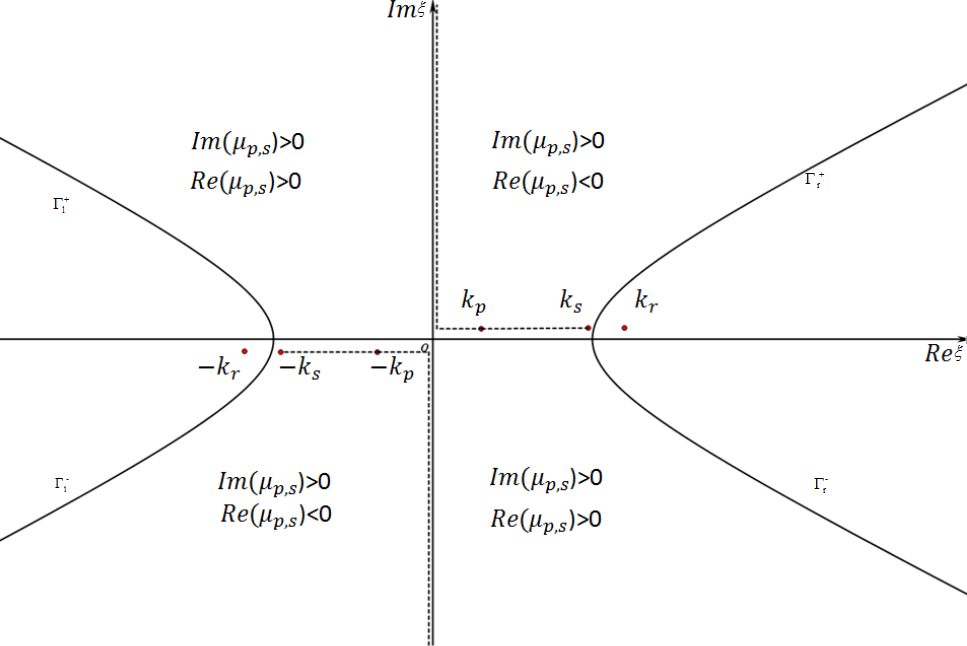
\includegraphics[width=0.8\textwidth]{./graphic/new_path.png}
	\caption{New Integration Path in the $\xi$-plane}\label{figure_newpath}
\end{figure}
Using Cauchy integral theorem and lemma \ref{root_De2}, we carry out:
\be
\N_\ep(x,y)=\frac{1}{2\pi}\int^{+\infty}_{-\infty}\hat \N_\ep(\xi,x_2;y_2) e^{\i(x_1-y_1)\xi} d\xi
\\
=\frac{1}{2\pi}\int_{NP}\hat N_\ep(\xi,x_2;y_2) e^{\i(x_1-y_1)\xi} d\xi\pm\i \mathit{Res}_{\xi=\pm k_R^\eps} N_\ep(\xi,x_2;y_2) e^{\i(x_1-y_1)\xi}
\ee
As the perturbation $\ep$ have nothing to do with the integration path $NP$, we could take the limitation $\ep\to0$. Therefore, we get the representation of Neumann Green Tensor
\be
\N(x,y)&=&\G(x,y)-\G(x,y')+\frac{1}{2\pi}\int_{NP}\hat \N_c(\xi,x_2;y_2) e^{\i(x_1-y_1)\xi}d\xi\\ \nn
&& \pm \i  {\mathit{Res}}_{\xi=\pm\kappa_r}  \hat \N_c(\xi,x_2;y_2) e^{\i(x_1-y_1)\xi}
\ee
where $\pm$ are corresponding $sgn(x_1-y_1)$.
Specially, $N(x,y)$ has a simple form when $x_2=0$:
\be \label{Ngreen}
\hspace{-2cm}
\N(x,y)&=&\frac{1}{2\pi}\int_{NP}\hat \N(\xi,0;y_2) e^{\i(x_1-y_1)\xi}d\xi
 \pm \i  {\mathit{Res}}_{\xi=\pm\kappa_r}  \hat \N(\xi,x_2;y_2) e^{\i(x_1-y_1)\xi}
\ee
where
\be \label{ngreen}
\hspace{-2cm}
\hat
        \N(\xi,0;y_2)&=&\frac{\i}{\mu\delta(\xi)} \Bigg[ \Bigg(
		\begin{array}{cc}
			2\xi^2\mu_s & -2\xi\mu_s\mu_p\\
			-\xi\beta & \mu_p\beta
		\end{array} \Bigg)e^{\i\mu_p y_2}
		+ \Bigg(
		\begin{array}{cc}
			\mu_s\beta & \xi\beta \\
			2\xi\mu_s\mu_p & 2\xi^2\mu_p
		\end{array} \Bigg)e^{\i\mu_s y_2} \Bigg] \\
	  &:=&\Np(\xi)e^{\i\mu_p y_2}+\Ns(\xi)e^{\i\mu_s y_2}
\ee
and let $\N_r(x_1;y_1,y_2)$ denote the first part of $N$ and $\N_s(x_1;y_1,y_2)$ denote the second part of $N$ in (\ref{Ngreen}).

It remains to study Dirichlet Green Tensor $\D(x,y)$.
 We still use Fourier transform to derive the formula of Green Tensor in frequency domain. Then we can obtain $\D(x,y)$ similar to $\N(x,y)$. It follows an alternative representation for $\D(x,y)$ 
\be
\hat \D(\xi,x_2;y_2) = \hat \G(\xi,x_2;y_2)  -\hat \G(\xi,x_2;-y_2) + \hat M(\xi,x_2;y_2)
\ee
\be
\hat
{M}(\xi,x_2;y_2)&=& \frac{\i}{\omega^2 \gamma(\xi)} \Bigg\{ A(\xi)e^{\i\mu_s(x_2+y_2)}+B(\xi)e^{\i\mu_p(x_2+y_2)}\\ \nn
&&-A(\xi)e^{\i\mu_s x_2+\mu_p y_2}-B(\xi)e^{\i\mu_p x_2+\mu_s y_2}\Bigg\}
\ee
where
\ben
    &&{A(\xi)} =
	\left( \begin{array}{ll}
	\xi^2\mu_s & -\xi\mu_s\mu_p \\
	-\xi^3  & \xi^2\mu_p
	\end{array} \right)\ \ \ \ \ \
	{B(\xi)} =
	\left( \begin{array}{ll}
	\xi^2\mu_s & \xi^3 \\
	\xi\mu_s\mu_p  & \xi^2\mu_p
	\end{array} \right)
\een
and $\gamma(\xi)=\xi^2+\mu_s\mu_p$.
\begin{lem} \label{root_Ga}
	Let \emph{Lam\'{e}} constant $\lambda, \mu \in \C$ and $\Im(k_s)\geq0, \Im(k_p)\geq0$, then equation $\gamma(\xi) = 0$ has no root in complex plane.
\end{lem}
\debproof
Let $F(\xi)= \gamma(\xi)*(\xi^2-\mu_s\mu_p)$ and it is easy to see that the root of $\gamma(\xi) = 0$ is also of $F(\xi)=0$. A simple computation show that $F(\xi)=(k_s^2+k_p^2)\xi^2-k_p^2 k_s^2$. However, only when $\xi^2=k_p^2 k_s^2 / (k_s^2+k_p^2)$, $F(\xi)=0$ but $\gamma(\xi)=2 k_p^2 k_s^2 / (k_s^2+k_p^2)$.
 This completes the proof.
\finproof
Thus, we get the representation of Green Tensor by inverse Fourier transform
\be
\D(x,y)&=&\G(x,y)-\G(x,y')+\frac{1}{2\pi}\int_{\R}\hat M(\xi,x_2;y_2) e^{\i(x_1-y_1)\xi}d\xi
\ee
Let $T_D(x,y)$ denote the traction of $\D(x,y)$ in direction $e_2$ with respect to $x$ such that $T_D(x,y)e_i=T_x^{e_2}(\D(x,y))e_i=T_x^{e_2}(\D(x,y)e_i)$. Then we can get the representation of $T_D(x,y)$ by a trivial calculation.
\be
T_D(x,y)&=&T(x,y)-T(x,y')+\frac{1}{2\pi}\int_{\R}\hat T_M(\xi,x_2;y_2) e^{\i(x_1-y_1)\xi}d\xi
\ee
and
\be
\hat
T_M(\xi,x_2;y_2)&=& \frac{\mathrm{\mu}}{\omega^2 \gamma(\xi)} \Bigg\{ E(\xi)e^{\i\mu_s(x_2+y_2)}+F(\xi)e^{\i\mu_p(x_2+y_2)}\\ \nn
&&-E(\xi)e^{\i\mu_s x_2+\mu_p y_2}-F(\xi)e^{\i\mu_p x_2+\mu_s y_2}\Bigg\}
\ee
where
\ben
		&&{E(\xi)} =
		\left( \begin{array}{cc}
			-\xi^2\beta & \xi\mu_p\beta \\
			2\xi^3\mu_s & -2\xi^2\mu_s\mu_p
		\end{array} \right)\ \ \ \
		{F(\xi)} =
		\left( \begin{array}{cc}
			-2\xi^2\mu_s\mu_p & -2\xi^3\mu_p \\
			-\xi\mu_s\beta  & -\xi^2\beta
		\end{array} \right)
\een
Specially, $T_D(x,y)$ has a simple form when $x_2=0$:
\be
T_D(x_1,0;y_1,y_2)=\frac{1}{2\pi}\int_{\R}\hat T_D(\xi,0;y_2) e^{\i(x_1-y_1)\xi}d\xi
\ee
where
\be\hspace{-1.5cm}
\hat
    T_D(\xi,0;y_2)&=&\frac{1}{\gamma(\xi)}\Bigg[\Bigg(   \begin{array}{cc}
	\mu_s\mu_p & \xi\mu_p \\
	\xi\mu_s & \xi^2
	\end{array}		\Bigg)e^{\i\mu_s y_2}+\Bigg(   \begin{array}{cc}
	\xi^2 & -\xi\mu_p \\
	-\xi\mu_s & \mu_p\mu_s
	\end{array} \Bigg)e^{\i\mu_p y_2}
	\Bigg]	\\
	 &:=&\Tp(\xi)e^{\i\mu_p y_2}+\Ts(\xi)e^{\i\mu_s y_2}
\ee

To analysis the point spread function in the section 5, we should give asymptotic anslysis for $N(x_1,0,y)$ and $T_D(x_1,0;y)$. We need the following slight generalization of Van der Corput lemma for the oscillatory integral \cite[P.152]{grafakos}.
\begin{lem}\label{van}
	Let $-\infty<a<b<\infty$, and $u$ is a $C^k$ function $u$ in $(a,b)$. \\
 1. If $|u'(t)|\ge 1$ for $t\in (a,b)$ and $u'$ is monotone in (a,b), then for any $\phi(t)$ in $(a,b)$ with integrable derivatives
	\ben
	\left|\int^b_a e^{\i\lambda u(t)}\phi(t)dt\right|\le
	3\lambda^{-1}\left[|\phi(b)|+\int^b_a|\phi'(t)|dt\right].
	\een
 2. For all $k\geq2$, if $|u^{(k)}(t)|\ge 1$ for $t\in (a,b)$ , then for any $\phi(t)$ in $(a,b)$ with integrable derivatives
	\ben
	\left|\int^b_a e^{\i\lambda u(t)}\phi(t)dt\right|\le
	12k\lambda^{-1/k}\left[|\phi(b)|+\int^b_a|\phi'(t)|dt\right].
	\een
\end{lem}
\debproof
The assertion can be proved by extending the Van der Corptut lemma in \cite{grafakos}. Here we omit the details.
\finproof
\begin{lem}\label{es_integral}
	Assume that $0<\kappa:=\sin\phi_\kappa<1,0<\phi_\kappa<\pi/2$, $0\leq\phi\leq\pi/2$. Let 
	\be
	f(t,\phi):=F(\sin(t+\phi),\cos(t+\phi),(\kappa^2-\sin^2(t+\phi))^{1/2})
	\ee
	be a complexed function in $C([-\pi/2,\pi/2]\times[0,\pi/2])$. Moreover, its partial derivative with respect to $t$ can be represented as
	\be\label{assume1}
	\frac{\pa f(t,\phi)}{\pa t}=g(t,\phi)(\kappa^2-\sin^2(t+\phi))^{-1/2}
	\ee 
	where $g(t,\phi)$ and $\pa g(t,\phi)/\pa t $ are uniformly bounded. Then for any $\rho\geq1$ and $\phi>\phi^*>\phi_\kappa$, we have
	\be\label{es_integral_1}
	\bigg|I(\rho,\phi):=\int_{-\pi/2}^{\pi/2}f(t,\phi)e^{\i\rho\cos t}dt\bigg| 
	\leq C\frac{1}{\rho^{1/2}}
	\ee	
	\be\label{es_integral_2}
	\bigg|H(\rho,\phi):=\int_{-\pi/2}^{\pi/2}\frac{\pa f(t,\phi)}{\pa t}e^{\i\rho\cos t}dt\bigg| 
	\leq C\frac{1}{\rho^{1/2}}
	\ee	
	where C is only dependent on $\kappa$ and $\phi^*$.
\end{lem}
\debproof
Since $\phi>\phi^*>\phi_\kappa$,  there exists $0<\delta<\pi/4$ such that
\be
|(\kappa^2-\sin^2(t+\phi))^{1/2}|>\frac{1}{2}|(\kappa^2-\sin^2\phi)^{1/2}|
\ee
for any $t\in(-\delta,\delta)$. Then we can divide $I$ into two parts such that
\ben
I=\int_{-\delta}^{\delta} f(t)e^{\i \rho\cos t} dt +
\int_{(-\frac{\pi}{2},\frac{\pi}{2})\bks[-\delta,\delta]} f(t) e^{\i \rho\cos t} dt  \\ 
=: I_{1} + I_{2}
\een
Similarly, we have $H=H_1+H_2$.
Let phase function $p(t)=\cos t$. It is easy to see that $|p''(t)|\geq \cos\delta$ for $t\in(-\delta,\delta)$ and $|p'(t)|\geq \sin\delta$. By lemma \ref{van}, we obtain
\be\hspace{-1.5cm}
 |I_1|&\leq& C\frac{1}{\rho^{1/2}}\left[|f(\delta,\phi)|+\int^\delta_{-\delta}|\frac{\pa f(t,\phi)}{\pa t}|dt\right]\leq C\frac{1}{\rho^{1/2}} \\  \hspace{-1.5cm}
 |I_2|&\leq& C \frac{1}{\rho} \left[|f(\frac{\pi}{2},\phi)|+|f(-\delta,\phi)|+\int_{(-\frac{\pi}{2},\frac{\pi}{2})\bks[-\delta,\delta]}|\frac{\pa f(t,\phi)}{\pa t}|dt\right]\leq C\frac{1}{\rho} \\ \hspace{-1.5cm}
 |H_1|&\leq& C\frac{1}{\rho^{1/2}}\left[|\frac{\pa f(\delta,\phi)}{\pa t}|+\int^\delta_{-\delta}|\frac{\pa^2 f(t,\phi)}{\pa^2 t}|dt\right]\leq C\frac{1}{\rho^{1/2}}
\ee
For $H_2(\rho,\phi)$, we can not use lemma \ref{van} again since ${\pa^2 f(t,\phi)}/{\pa^2 t}$ is not integrable on $(-\frac{\pi}{2},\frac{\pi}{2})\bks[-\delta,\delta]$. 
	Solving the following equation:
\ben
\kappa^2-\sin^2(t+\phi)=0
\een
we have, if $0<\phi<\pi/2-\phi_\kappa$,
\ben
t_1(\phi)=\phi_\kappa-\phi \ \ \ \ \ t_2(\phi)=-\phi_\kappa-\phi
\een
and if $\pi/2-\phi_\kappa\leq\phi<\pi/2$,
\ben
t_1(\phi)=\phi_\kappa-\phi  \ \ \ \ \ t_2(\phi)=\pi-\phi_\kappa-\phi
\een
However,  for any $0<\lambda_1<1$ and $1<\lambda_2<1/\kappa$, there exists $\sigma>0$, such that $\chi:=((t_1-\sigma,t_1+\sigma)\cup(t_2-\sigma,t_2+\sigma))\subset (-\frac{\pi}{2},\frac{\pi}{2})\bks[-\delta,\delta]$, dependent on $\lambda_1,\lambda_2$ and
\be \label{assume2}
\lambda_1\kappa<|\sin (t+\phi)|<\lambda_2\kappa.
\ee
for any $t\in\chi$. 

We only analysis the integral on $\chi_{1}=(t_1-\sigma,t_1+\sigma)\cap[-\pi/2,\pi/2]$ here, which denoted by $H_{\chi_1}$, the proof of $H_{\chi_2}$ is similar. It is easy to see that $\sin (t+\phi)$ is monotonic in $\chi_1$. Without loss of generality, we assume that $\sin (t_1-\sigma+\phi)<\kappa<\sin (t_1+\sigma+\phi)$. Let $\sin (t+\phi) = \kappa \sin \theta$ and the implicit mapping from $\theta$ to $t$ is denoted by $t(\theta)$ while the inverse mapping by $\theta(t)$, taking the interval $\chi_1$ onto $L_\theta : \theta_1\rightarrow\pi/2\rightarrow\pi/2-\i\theta_2$ where $\sin(t_1-\sigma+\phi)=\kappa\sin \theta_1,\sin(t_1+\sigma+\phi)=\kappa\sin(\pi/2-\i\theta_2)$. By substituting $t(\theta)$ into $H_{\chi_1}$, we have
\be
H_{\chi_1}&=&\int_{t_1-\sigma}^{t_1+\sigma}\frac{g(t,\phi)}{(\kappa^2-\sin^2(t+\phi))^{1/2}} e^{\i\rho\cos t}\\
&=&\int_{L_\theta}\frac{g(t(\theta),\phi)}{(1-\kappa^2\sin^2\theta)^{1/2}}e^{\i
	\rho(\cos(t(\theta)))} d\theta 
\ee
Observe that $h(\theta)$ and $\pa h/\pa\theta$ are integrable on the path $L_\theta$ by (\ref{convention_1}). A simple computation show that
\ben\hspace{-0.5cm}
\frac{dt(\theta)}{d\theta}=\frac{\kappa\cos\theta}{\cos(t+\phi)} \ \ \ \ \ \
\frac{d^2 t(\theta)}{dt^2}=\frac{\kappa^2\cos^2\theta\sin(t+\phi)-\kappa\sin\theta\cos^2(t+\phi)}{\cos^3(t+\phi)}
\een
Then we can obtain
\ben
\frac{d\cos t}{d\theta}&=&\frac{-\kappa\sin t\cos\theta}{\cos(t+\phi)} \\
\frac{d^2\cos t}{d\theta^2}&=&\frac{d^2\cos t}{dt^2}(\frac{dt}{d\theta})^2+\frac{d\cos t}{dt}\frac{d^2t}{d\theta^2} \\
&=&\frac{-\kappa^2\cos^2\theta\cos t}{\cos^2(t+\phi)}+\frac{\kappa\sin\theta\cos^2(t+\phi)\sin t -\kappa^2\cos^2\theta\sin(t+\phi)\sin t}{\cos^3(t+\phi)} \\
&=&\frac{-\kappa^2\cos^2\theta\cos\phi+\kappa\sin\theta\cos^2(t+\phi)\sin t}{\cos^3(t+\phi)} \\
&=&\frac{(\sin^2(t+\phi)-\kappa^2)\cos\phi+\cos^2(t+\phi)\sin(t+\phi)\sin t}{\cos^3(t+\phi)}
\een
Since $|\sin t|>|\sin\delta|$ and $1-\lambda_2^2\kappa^2<\cos^2(t+\phi)<1-\lambda_1^2\kappa^2$ for $t\in\chi_1$, it follows that $\theta=\pi/2$ is the only stationary point of $\cos(t(\theta))$ and 
\be
\Bigg|\frac{d^2\cos t}{d\theta^2}(\pi/2)\Bigg|=\frac{(1-\kappa^2)\kappa}{(1-\kappa^2)^{3/2}}|\sin t|>\frac{(1-\kappa^2)\kappa}{(1-\kappa^2)^{3/2}}\sin \delta
\ee
Therefore, we can choose appropriate $\lambda_1,\lambda_2$ such that 
\be
|\frac{d^2\cos t}{d\theta^2}|>\frac{(1-\kappa^2)\kappa}{(1-\kappa^2)^{3/2}}\sin \delta
\ee
for any 
$\theta\in \theta(\chi_1)$. According to lemma (\ref{van}), we obtian $|H_{\chi_1}|\leq C\frac{1}{\rho^{1/2}}$, and also $|H_{\chi_2}|\leq C\frac{1}{\rho^{1/2}}$. Using integration by parts, we get
\ben
\Bigg|\int_{[-\pi/2,\pi/2]\bks((-\delta,\delta)\cup\chi)}\frac{\pa f(t,\phi)}{\pa t} e^{\i \rho\cos t} dt\Bigg| 
\leq C\frac{1}{\rho}
\een
Finally, combining above inequality, we arrive at the estimate. This completes the proof.


\finproof
Therefore, the estimate of $T_D(x_1,0;y_1,y_2)$ and $N(x_1,0;y_1,y_2)$ are now direct consequence of lemma \ref{es_integral}.
\begin{lem}\label{es_dgreen}
	For every $x\in\Gamma_0$, $y\in\R_+^2$ such that $|x_1-y_1|/|x-y|>(1+\kappa)/2$, $y_2/|x-y|<\kappa/2$ and $k_s |x-y|>1$, we have
	\be\hspace{-1.5cm}
	|T_D(x,y)|\leq C\Bigg(\frac{k_s y_2}{|x-y|}\frac{1}{(k_s|x-y|)^{1/2}}+\frac{k_s |x_1-y_1|}{|x-y|}\frac{1}{(k_s|x-y|)^{3/2}}\Bigg)
	\ee
	where C is only dependent on $\kappa$.
\end{lem}
\debproof
Put
\be
I(|x_1-y_1|,y_2)=\int_\R \Ts(\xi) e^{\i(\mu_s y_2 + \xi |x_1-y_1|) } d\xi \\
J(|x_1-y_1|,y_2)=\int_\R \Tp(\xi) e^{\i(\mu_p y_2 + \xi |x_1-y_1|) } d\xi
\ee
To simplify the integral $I$, the standard substitution $\xi=k_s\sin t$ is made, taking the $\xi$-plane to a strip $-\pi<\Re t <\pi$ in the t-plane, and the real axis in the $\xi$-plane onto the path L from $-\pi/2+\i\infty\rightarrow-\pi/2\rightarrow\pi/2\rightarrow\pi/2-\i\infty$ in the t-plane. The integral $I(|x_1-y_1|,y_2)$ then becomes (Let $|x_1-y_1|=\rho \sin\phi$  and $y_2=\rho\cos\phi$, $0<\phi<\pi/4$):
\be
k_s \int_L F(\sin t,\cos t,(\kappa^2-\sin^2 t)^{1/2})\cos t \ e^{\i k_s\rho(\cos (t-\phi))} dt
\ee
where $ F(\sin t,\cos t,(\kappa^2-\sin^2 t)^{1/2})=\Ts(k_s \sin t) $.
Taking the shift transformation of t and using cauchy integral theorem, we can get the representation of I:
\ben \hspace{-1.5cm}
k_s\int_L F(\sin (t+\phi),\cos (t+\phi),(\kappa^2-\sin^2 (t+\phi))^{1/2})\cos (t+\phi) e^{\i k_s\rho(\cos t)} dt \\\hspace{-2cm}
=k_s \cos \phi \int_L F(\sin (t+\phi),\cos (t+\phi),(\kappa^2-\sin^2 (t+\phi))^{1/2})\cos t \ e^{\i k_s\rho(\cos t)} dt \\\hspace{-2cm}
-k_s \sin \phi \int_L F(\sin (t+\phi),\cos (t+\phi),(\kappa^2-\sin^2 (t+\phi))^{1/2})\sin t \ e^{\i k_s\rho(\cos t)} dt \\\hspace{-2cm}
:=k_s (\cos\phi \ I_1+\sin\phi \ I_2)
\een
For $I_1$, we split the integral path L into $L_1=(-\pi/2,\pi/2)$ and $L_2=(-\pi/2+\i\infty,-\pi/2)\cup(\pi/2,\pi/2-\i\infty)$, then we have corresponding representation: $I_1=I_{11}+I_{12}$. Since $F(t)\cos t$ satisfy (\ref{assume1}), we can obtain $|I_{11}|\leq 1/(k_s\rho)^{1/2}$ by lemma \ref{es_integral}. Using integration by parts, it follows that $|I_{12}|\leq 1/(k_s\rho)$.
For $I_2$, using integration by parts on path $L$ first, we have
\be \hspace{-2cm}
I_2=\frac{1}{\i k_s\rho} \int_L F(\sin (t+\phi),\cos (t+\phi),(\kappa^2-\sin^2 (t+\phi))^{1/2}) d \ e^{\i(k_s\rho \cos t)} \\ \hspace{-1.5cm}
=-\frac{1}{\i k_s\rho} \int_{L_1 \cup L_2} \frac{\pa F(\sin (t+\phi),\cos (t+\phi),(\kappa^2-\sin^2 (t+\phi))^{1/2})}{\pa t
} \  e^{\i(k_s\rho \cos t)} dt \\ \hspace{-1.5cm}
=-\frac{1}{\i k_s\rho}(I_{21}+I_{22})
\ee
Similarly, we have $|I_{21}+I_{22}|\leq 1/(k_s\rho)^{1/2}$ by lemma \ref{es_integral}.
The estimate of $J(|x_1-y_1|,y_2)$ can be proved by the same method as employed above.
This completes the proof.
\finproof
\begin{lem}\label{es_ngreen}
	For every $x\in\Gamma_0$, $y\in\R_+^2$ such that $|x_1-y_1|/|x-y|>(1+\kappa)/2$, $y_2/|x-y|<\kappa/2$ and $k_s |x-y|>1$, we have
	\be\hspace{-2.5cm}
	|N(x,y)|\leq \frac{C}{\mu}\Bigg(\frac{ y_2}{|x-y|}\frac{1}{(k_s|x-y|)^{1/2}}+\frac{ |x_1-y_1|}{|x-y|}\frac{1}{(k_s|x-y|)^{3/2}}+e^{-\sqrt{k_R^2-k_s^2}y_2}\Bigg)
	\ee
	where C is only dependent on $\kappa$.
\end{lem}
\debproof
The proof is similar to lemma \ref{es_dgreen}. Here we only point out the different parts. Notice that, in the present case, the substitution $\xi=k_s \sin t$ , taking $\Gamma_r^+$ in the $\xi$-plane onto $L_r:=\{t=t_1+\i t_2|\cos(2t_1)\cosh(2t_2)=-1,\frac{\pi}{2}\leq t_1<\frac{3\pi}{4},t_2\leq 0\}$ in the $t$-plane and  $\Gamma_l^+$ in the $\xi$-plane onto $L_l:=\{t=t_1+\i t_2|\cos(2t_1)\cosh(2t_2)=-1,-\frac{\pi}{2}\leq t_1<-\frac{1\pi}{4},t_2\geq 0\}$ in the $t$-plane.   To see this transformation, observe that since 
\ben
\sin t =\cosh t_2\sin t_1+\i \sinh t_2 \cos t_1 \\
\cos t=\cosh t_2\cos t_1-\i \sinh t_2 \sin t_1
\een
 we have
\ben
L_r&=&\{t=t_1+\i t_2 \ | \ \cosh^2 t_2\sin^2 t_1 - \sinh^2 t_2 \cos^2 t_1=1,\frac{\pi}{2}\leq t_1<\pi,t_2\leq0 \} \\
&=&\{t=t_1+\i t_2 \ | \ \frac{e^{2t_2}+e^{-2t_2}}{2}(\sin^2 t_1-\cos^2 t_1)=1,\frac{\pi}{2}\leq t_1<\pi,t_2\leq0 \} \\
&=&\{t=t_1+\i t_2|\cos(2t_1)\cosh(2t_2)=-1,\frac{\pi}{2}\leq t_1<\frac{3\pi}{4},t_2\leq 0\}
\een
The same procedure is adopted for $L_l$. The geometry now is depicted in Figure \ref{figure_trans}.
\begin{figure}
	\centering
	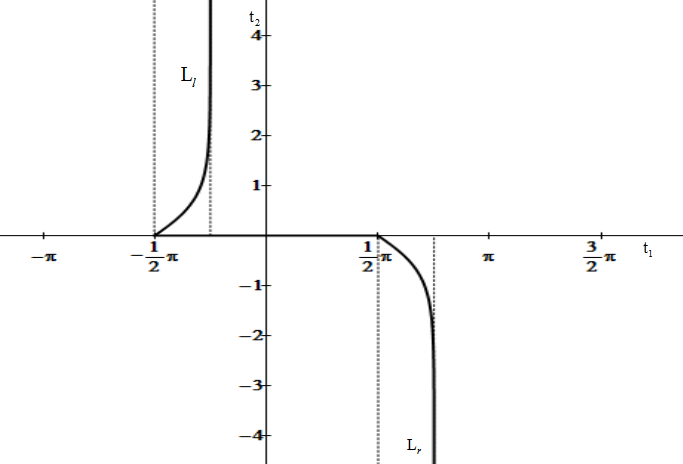
\includegraphics[width=0.8\textwidth]{./graphic/transformation.png}
	\caption{Transform from $\Gamma_l^+\cup(-k_s,k_s)\cup\Gamma_r^+$ to $L_l\cup (-\pi/2,\pi/2)\cup L_r$}\label{figure_trans}
\end{figure}
Put
\ben I
=\int_{L_r} k_s\Ns(k_s \sin(t+\phi))\cos t e^{\i k_s \rho \cos t} dt
\een
By equation (\ref{ngreen}), it is easy to see that for $t\in L_r$
\ben\hspace{-2cm}
k_s|\Ns(k_s\sin(t+\phi))\cos t|\leq C(1+|\sin^3(t+\phi)\cos(t+\phi)|)\leq C(1+\cosh^4(t_2))
\een
Direct computation show that for $t\in L_r$
\ben
\frac{dt_1}{dt_2}=\frac{\cos(2t_1)\sinh(2t_2)}{\sin(2t_1)\cosh(2t_2)}=-\frac{\cos(2t_1)\sqrt{\cosh^2(2t_2)-1}}{\sin(2t_1)\cosh(2t_2)}=\frac{1}{\cosh(2t_2)}
\een
Thus
\ben
|I|\leq C\int_{-\infty}^{0}(1+\cosh^4(t_2))\sqrt{\frac{1}{\cosh^2(2t_2)}+1} \ \
e^{\frac{\sqrt{2}}{2}k_s \rho\sinh(t_2)}dt_2
\een
Let $s=-\sinh(t_2)$, then for $k_s\rho>1$ we have
\be
|I|\leq C\int_{0}^{\infty}(1+(1+s^2)^2)/\sqrt{1+s^2}e^{-\frac{\sqrt{2}}{2}k_s \rho s}ds\leq C\frac{1}{k_s\rho}
\ee
Similarly, we can also obtain
\ben
|\int_{L_r}\frac{\pa \Ns(k_s\sin(t+\phi))}{\pa t}e^{\i k_s \rho \cos t} dt|\leq C\frac{1}{k_s\rho}
\een
Therefore, the proof of this lemma can be completed  by the same method as employed in the lemma \ref{es_dgreen}. Here we omit the details.
\finproof

\section{The forward scattering problem}

In this section we introduce the following stability estimate of the forward elastic scattering problem in the half space which can be proved by the limiting absorption principle by extending the classical argument in \cite{leis,wilcox1975,Yves1988}.
\begin{thm} \label{elastic_eq2}
	Let $g \in H^{1/2}(\Ga_D)$, then the scattering problem of elastic equation in the half space
	\be
	\Delta_e \u + \omega^2 \u =0 \qquad\mbox{\rm in } \R^2_+\bks \bar{D}, \label{elas_1}\ \ \
	\\ \u= g \ \ \ \ \mbox{\rm on } \Ga_D, \label{elas_bd} \\
	\sigma(\u)e_2=0 \ \ \ \ \mbox{\rm on} \Ga_0, \label{elas_b0} \\
	\u \ \mbox{satisfies the generalized radiation codition\cite{Guzina2006} such that} \nn \\\label{rc}
	\lim_{r\to\infty}  \int_{S_r^+} (\sigma(N(x,y)e_i)\hat{r})\cdot \u(x) - (N(x,y)e_i)\cdot (\sigma(\u)\hat{r})ds(x)=0
	\ee
	where $S_r^+:=\{x\in \R^2_+ \ | \ \|x\|=r^2\}$, $\hat{r}=x/r$ and $y\in \R_+^2$. Then the problem (\ref{elas_1})-(\ref{rc})
	admits a unique solution $\u \in H^{1}_{\rm loc}(\R^2_+ \backslash \bar D)$. Moreover, for any bounded open set $\mathcal O\subset \R^2_+\bks\bar D$ there exists a constant $C>0$ such that
	\be \label{elas_ineq}
	\|\u\|_{H^{1}(\mathcal O)}\le C\|g\|_{H^{-1/2}(\Ga_D)}
	\ee
\end{thm}
The existence of the solution can be proved by the method of limiting absorption principle. The argument is standard and we give several lemmas below, see e.g. \cite{leis} for the consideration for Helmholtz equation. For any $z=1+\i\ep,\ep>0$, $f\in H^{1}(\R^2_+)'$ with compact support in $B_R=\{x||x|^2<R^2,x\in\R^2_+\}\subsetneq\R_+^2$ where $B_R$ is an half disc of radius R , we consider the problem
\be \label{elastic_eqz}
\Delta_e \u_z +z\omega^2 \u =-f \qquad\mbox{\rm in } \R^2_+ \\
\sigma(\u_z)e_2=0 \ \ \ \ \mbox{\rm on} \ \ \ \  \Ga_0 \label{elastic_b0}
\ee
By Lax-Milgrim lemma we know that (\ref{elastic_eqz}-\ref{elastic_b0}) has a unique solution $\u_z\in H^1(\R^2_+)$. For any domain $ D \subset \R^2_+$, we define the weighted space $L^{2,s}(D),s \in \R$, by
\ben
L^{2,s}(D)=\{v \in L^2_{\rm loc}(D): (1+|x|^2)^{s/2}v \in L^2(D) \}
\een
with the norm $\| v \|_{ L^{2,s}(\mathcal D)} = (\int_{\mathcal D}(1+|x|^2)^{s}|v|^2 dx )^{1/2}$. The weighted Sobolev space $H^{1,s}(D),s \in \R$,
is defined as the set of functions in $L^{2,s}(D)$ whose first derivative is also in $L^{2,s}(D)$. The norm
$\| v \|_{ H^{1,s}(D)} = (\| v \|^2_{ L^{2,s} (D)} + \| \nabla v \|^2_{ L^{2,s}(D)})^{1/2}$.

We need the following sligt generalization of Rellich Theorem:
\begin{lem}\label{relli_embed}
	Let $\Omega$ be an open Lipschitz domain, then the sobolev space $H^{1,-s}(\Omega)$ is compactly embeded in $L^{2,-s'}(\Omega)$ for every $s'>s>0$.
\end{lem}

\begin{lem}{\label{global_es}}
	Let  $ f  \in L^2 (\R^2_+) $ with compact support in $B_R$. For any $z=1+\i\ep$, $0<\ep<1$, we have, for any $s>1/2$,
	$\|\u_z\|_{H^{1,-s}(\R^2_+)}\le C\|f\|_{L^2(\R^2_+)}$ for some constant independent of $\ep, u_z$, and $f$.
\end{lem}
\debproof
Let $R_z$ denote the map from $L^2_c(\R^2_+)$ to $H^{1,-s}(\R^2_+)$ such that $R_z(f)=\u_z$ where $L^2_c(\R^2_+)$ is denoted by all $ f  \in L^2 (\R^2_+) $ with compact support in $B_R$, then it is easy to see that $R_z$ is a linear bounded operator. It follows from theorem 3.7 in \cite{Yves1988} that $R_z$ is a uniformly continuous operator continues valued function on $z=1+\i\ep$, $0<\ep<1$ with value in $B(L^2_c(\R^2_+),H^{1,-s}(\R^2_+))$. Then, we can obtain that $R_z$ is uniformly bounded in $B(L^2_c(\R^2_+),H^{1,-s}(\R^2_+))$. This complete the proof by the defintion of the operator norm.
\finproof

We next recall the following lemma which states the absence of positive eigenvalues for the linear elasticity system in half space \cite{sini2004}.
\begin{lem} \label{elas_unique}
	Let $\u\in L^2(\R^2_+ \backslash \bar D)$ such that $u$ satisfies (\ref{elas_1}) and (\ref{elas_b0}), than we assert that $u=0$ in $\R^2_+ \backslash \bar D$
\end{lem}
\debproof
The asserting above can be proved by extending \cite[theorem 3.1]{sini2004}, here we omit the details.
\finproof

For any $0<\ep<1$, we consider the problem
\be {\label{elas_z1}}
\Delta_e \u_\ep + (1+\i\ep)\omega^2 \u_\ep=0 \qquad\mbox{\rm in } \R^2_+\bks \bar{D}\\
\u_\ep= g \ \ \ \ \mbox{\rm on } \Ga_D  \label{elas_zbd}\\
\sigma(\u_\eps)e_2=0 \ \ \ \ \mbox{\rm on} \Ga_0 \label{elas_zb0}
\ee
We know that the above problem has a unique solution $\u_{\ep} \in H^1(\R^2_+ \backslash \bar D)$ by the Lax-Milgram Lemma. Thus, we have next lemma
\begin{lem}{\label{global_elas_bd}}
	Let  $ g  \in H^{1/2} (\Ga_D) $ . For any $0<\ep<1$, we have, for any $s>1/2$,
	$\|\u_{\eps}\|_{H^{1,-s}(\R^2_+ \backslash \bar D)} \leq C \|g\|_{H^{1/2}(\Ga_D)}$ for some constant independent of $\ep, \u_\eps$, and $g$.
\end{lem}
\debproof
Because $h=dist(D,\Ga_0)>0$, we can find three concentric circles $B_{R_1},B_{R_2},B_{R_3}$ such that $D\subsetneq B_{R_1}\subsetneq B_{R_2} \subsetneq B_{R_3} \subsetneq \R^2_+$. Let $\chi \in C_{0}^{\infty}(\R^2_+)$ be the cut-off function such that $0 \leq \chi \leq 1$, $\chi=0$ in $B_{R_1}$, and $\chi=1$ outside of $B_{R_2}$.
Let $v_\eps=\chi \u_\eps$.
Then $v_\eps$ satisfies (\ref{elastic_eqz}) with
$z=1+\i\eps$ and $q=\sigma(\u_\eps)\na\chi+(\lambda+\mu)(\na^2 \chi \u_\eps+ \na \u_\eps \na\chi)+\mu\Delta\chi \u_\eps +\mu\div \u_\eps\na\chi$, where $\na^2 \chi$ is the Hessian matrix of $\chi$. Clearly $q$ has compact support. By lemma \ref{global_es} we can obtain
\be \label{elas_ineq2}
\|v_\eps\|_{H^{1,-s}(\R^2_+)}\le C\|\u_{\eps}\|_{H^1(B_{R_2}\backslash \bar{D})}
\ee
for some constant $C$ independent of $\eps>0$. Now let $\chi_1 \in C_{0}^{\infty}(\R^2_+)$
be the cut-off function with that  $0 \leq \chi_1 \leq 1$, $\chi_1=1$ in $B_{R_2}$, and $\chi_1=0$
outside of $B_{R_3}$. For $g\in H^{1/2}(\Ga_D)$, let $\u_g \in H^{1}(\R^2_+ \backslash \bar{D})$ be the lifting function such that $  \u_{g}=g \mbox{ on } \Ga_D$ and $\|\u_{g}\|_{H^{1}(\R^2_+ \backslash \bar{D})}\le C\|g\|_{H^{1/2}(\Ga_D)}$. By testing \ref{elas_z1} with
$\chi_1^2 ( \overline{\u_{\eps}-\u_{g}} )$ and using the standard argument we have
\be \label{elas_ineq3}
\|\u_{\eps}\|_{H^{1}(B_{R_2} \backslash \bar{D})}\le C( \|\u_{\eps}\|_{L^{2}(B_{R_3} \backslash \bar{D})} + \|g\|_{H^{1/2}(\Ga_D)} ).
\ee
A combination of (\ref{elas_ineq2}) and the above estimate yields
\be \label{elas_ineq4}
\|\u_{\eps}\|_{H^{1,-s} ( \R^2_+ \backslash \bar{D})}\le C( \|\u_{\eps}\|_{L^{2}(B_{R_3} \backslash \bar{D})} + \|g\|_{H^{1/2}(\Ga_D)} ).
\ee
Now we claim
\be \label{elas_ineq5}
\|\u_{\eps}\|_{L^2(B_{R_3} \backslash \bar D)} \leq C \|g\|_{H^{1/2}(\Ga_D)} ,
\ee
for any $g \in H^{1/2}(\Ga_D)$ and $\eps >0$. If it were false, there would exist sequences $\{g_m\} \subset H^{1/2}(\Ga_D)$ and $\{\eps_m\} \subset (0,1)$, and $\{\u_{\eps_m}\}$ be the corresponding solution of (\ref{elas_z1})-(\ref{elas_zb0}) such that
\be {\label{contradict}}
\|\u_{\eps_m}\|_{L^2(B_{R_3} \backslash \bar D)} = 1 \ {\rm{ and }} \ \|g_m\|_{H^{-1/2}(\Ga_D)} \leq \frac{1}{m}.
\ee
Then $\|\u_{\eps_m}\|_{H^{1,-s} ( \R^2_+ \backslash \bar{D})}\le C $, and thus there is a subsequence of $\{\eps_m\}$, which is
still denoted by $\{\eps_m\}$, such that $\eps_m \to \eps' \in [0,1]$, and a subsequence of $\{\u_{\eps_m}\}$,
which is still denoted by $\{\u_{\eps_m}\}$, such that it converges to some $\u_{\eps'}$ in ${H^{1,-s'} ( \R^2_+ \backslash \bar{D})}$ by choosing $s'>s$. This is a consequence of Korn's inequality and lemma \ref{relli_embed}. So $\u_{\eps'} \in H^{1,-s'}(\R^2_+ \backslash \bar D)$ satisfies (\ref{elas_z1}-\ref{elas_zb0}) with $g=0$ and $\eps=\eps'$.

By the integral representation satistied by $\u_{\eps_m}$, we know that for $y\in \R^2_+\backslash\bar B_{R_1}$ and $i=1,2$
\be \ \hspace{-2cm} \label{green_rep}
\u_{\eps'}(y)\cdot e^i=\int_{\pa B_{R_1}} (\sigma(\N_{\eps'}(x,y)e_i)\nu)\cdot \u_{\eps'}(x) - (\N_{\eps'}(x,y)e_i)\cdot (\sigma(\u_{\eps'})_{\eps'}\nu)ds(x)
\ee
If $\eps'>0$, we deduce  from (\ref{green_rep}) that $\u_{\eps'}$ decays exponentially and thus $\u_{\eps'} \in H^{1}(\R^2_+\backslash \bar D) $, then $\u_{\eps'} =0$ by the uniqueness of the solution in $H^{1}(\R^2_+ \backslash \bar D) $ with positive absorption.
If $\eps'=0$, by the \cite[theorem 5.2]{Yves1988}, we have $\u_{\eps'}\in L^2(\R^2_+\bks\bar D)$. Then we conclude $\u_{\eps'}=0$ by the lemma \ref{elas_unique}
Therefore, in any case $\u_{\epsilon'}=0$, which , however contradicts to \ref{contradict}. This complete the proof.
\finproof
Now we are in the position to prove the exsitence of Theorem \ref{elastic_eq2}.
\begin{lem} \label{elas_exis}
	For any $s>1/2$, $\u_\eps:(0,1)\to H^{1,-s}(\R^2_+ \bks \bar D)$ is a uniformly continuous operator valued function. Immediately, $\u_{\eps}$ converges to some $\u_0$ in $H^{1,-s}(\R^2_+ \bks \bar D)$ and $\u_0$ is a solution of (\ref{elas_1}-\ref{elas_ineq}).
\end{lem}
\debproof
We also give a indirect prove here. Let $\delta_0>0$ and $\{\mu_n\}$ and $\{\nu_n\}$ be sequences in $ (0,1) $ such that
\be
|\mu_n-\nu_n|\le 1/n \qquad \mbox{and} \qquad \|\u_{\mu_n}-\u_{\nu_n}\|_{H^{1,-s}(\R^2_+ \bks \bar D)} \ge \delta_0
\ee
Thus there is a subsequence of $\{\mu_n\}$, which is still denoted by $\{\mu_n\}$, such that $\{\mu_n\}\to \epsilon\in[0,1]$ and also $\{\nu_n\}\to \epsilon$. Then using lemma \ref{global_elas_bd} and the procedure proving it, we get the $u_\epsilon,v_\epsilon \in H^{1,-s'} (\R^2_+ \bks \bar D)$, by choosing $s'>s$, such that
\ben
\|u_{\mu_n}-u_\epsilon\|_{H^{1,-s'}(\R^2_+ \bks \bar D)} \to 0 \\
\|u_{\nu_n}-v_\epsilon\|_{H^{1,-s'}(\R^2_+ \bks \bar D)} \to 0
\een
and $u_\epsilon=v_\epsilon$ by the same arguement in lemma \ref{global_elas_bd} which leads to a contradiction. Thus we have proved $u_\eps$ is uniformly continuously for $\eps \in (0,1)$. Then it is easy to see $u_\eps$ has a limitation in ${H^{1,-s}(\R^2_+ \bks \bar D)} $ and the estimation of $u_0$ can be obtained by (\ref{elas_ineq5}). This completes the proof.
\finproof
It is remain to prove the uniqueness in theorem \ref{elastic_eq2}. Actually, it can be obtained following the existence of solution with any $g\in H^{1/2}(\Ga_D)$.

{\it \bf proof of Theorem \ref{elastic_eq2}}
By the linearity of the problem, it is sufficient to prove that any $u_0$  satisfies the system (\ref{elas_1}-\ref{elas_b0}) with the corresponding homogeneous boundary-value vanishes identically in $\R^2_+\bks \bar D$. For any $y\in \R^2_+\bks \bar D$, there exists $U^s(x,y)$ sataifies (\ref{elas_1}-\ref{elas_b0}) with $g(x)=-\N(x,y)$ on $\Ga_D$ following the lemma \ref{elas_exis} and we define $U(x,y)=N(x,y)+U^s(x,y)$. It is easy to see that $\u(x,y)$ satifies the generalized radiation condition (\ref{rc}). Thus by the integral representaion of $\u_0$, we have
\ben
\lim_{r\to\infty}  \int_{S_r^+} (\sigma(U(x,y)e_i)\nu)\cdot \u_0(x) - (U(x,y)e_i)\cdot (\sigma(\u_0)\nu)ds(x)=0
\een
Finally, combining $U(x,y)=0,\u_0(x)=0$ on $\Ga_D$ and the Green integral theorem we find that
\ben
\u_0(y)e_i&=\int_{\R^2_+\bks\bar D} -(\Delta_e (\N(x,y)e_i)+\omega^2 \N(x,y)e_i)\cdot \u_0(x) dx\\
&=\int_{\R^2_+\bks\bar D} \Delta \u_0(x)\cdot (\N(x,y)e_i)
-\Delta_e (\N(x,y)e_i)\cdot \u_0(x) \\
&=\int_{\Ga_D} (\sigma(U(x,y)e_i)\nu)\cdot \u_0(x) - (U(x,y)e_i)\cdot (\sigma(\u_0)\nu)ds(x)=0
\een
Then the desired unique exsitence follows lemma \ref{elas_exis}. This completes the proof of theorem \ref{elastic_eq2}.
\finproof


\section{Reverse time migration method}
In this section we introduce RTM method for inverse elastic scattering problems in the half space. Assume that there $N_s$ sources and $N_r$ receivers uniformly distributed on $\Gamma^d_0$, where $\Gamma^d_0=\{(x_1,x_2)^T\in\Gamma_0:x_1\in[-d,d]\},d>0$ is aperture. We denote by $\Omega$ the sampling domain in which the obstacle is sought. Let $h=dist(\Omega,\Gamma_0)$ be the distance of $\Omega$ to $\Gamma_0$. We assume the obstacle $D\subset\Omega$ and there exist constants $0<c_1<1,c_2>0,c_3>0$ such that
\be\label{convention_2}
|x_1|\leq c_1 d , \ \ |x_1-y_1|\leq c_2 h , \ \
|x_2|\leq c_3 h    \ \ \ \forall x,y \in \Omega
\ee

Our RTM algorithm consists of two steps \cite{ela_reverse,Zhang08,Zhang2007}. The first step is the back-propagation in which we back-propagate the complex conjugated data $\overline{\u^s(x_r,x_s)}$ as the Dirichlet boundary condition into the domain. The second step is the cross-correlation in which we compute the imaginary part of the cross-correlation of the back-propagated field and the incoming wave which uses the source as the boundary codition on $\Gamma_0$.
\begin{alg}{\sc (Reverse time migration algorithm)}\label{alg_rtm}\\
Given the data $u_k^s(x_r,x_s)$, $k=1,2$ which is the measurement of the scattered field at $x_r$ when the source is emitted at $x_s$ along the  polarized direction $e_k$, $s=1,\dots, N_s$ and $r=1,\dots,N_r$. \\	
$1^\circ$ Back-propagation: For $s=1,\dots,N_s$ and k=1,2, compute the back-propagation field
\be
v_k(z,x_s)=\frac{|\Gamma_0^d|}{N_r}\sum^{N_r}_{r=1}(T^{e_2}_{x_r}\D(x_r,z))^T\overline{\u^s_k(x_r,x_s)}, \ \ \ \ \ \forall z\in\Omega
\ee
$2^\circ$ Cross-correlation: For $z\in\Om$, compute
\be\label{cor1}
I_d(z)=\Im\sum_{k=1}^{2}\left\{\frac{|\Gamma_0^d|}{N_s}\sum^{N_s}_{s=1}[(T^{e_2}_{x_s}\D(x_s,z))^Te_k]\cdot v_k(z,x_s)\right\}.
\ee
\end{alg}

It is easy to that for $z\in\Om$
\be\hspace{-2.5cm}\label{cor2}
I_d(z)=\Im\sum_{k=1}^{2}\left\{\frac{|\Gamma_0^d|}{N_s}\frac{|\Gamma_0^d|}{N_r}\sum^{N_s}_{s=1}\sum^{N_r}_{r=1}[(T^{e_2}_{x_s}\D(x_s,z))^Te_k]\cdot[(T^{e_2}_{x_r}\D(x_r,z))^T\overline{\u^s_k(x_r,x_s)}]\right\}
\ee
This formula is used in all our numerical experiments in section. By letting $N_s,N_r\to\infty$, we know that (\ref{cor2}) can be viewed as an approximation of the following continuous integral:
\be\hspace{-2.5cm}\label{cor3}
\hat{I}_d(z)=\Im\sum_{k=1}^{2}\int_{\Gamma_0^d}\int_{\Gamma_0^d}[(T^{e_2}_{x_s}\D(x_s,z))^Te_k]\cdot[(T^{e_2}_{x_r}\D(x_r,z))^T\overline{\u^s_k(x_r,x_s)}]ds(x_r)ds(x_s)
\ee
where $z\in\Om$. We will study the resolution of the function $\hat{I}_d(z)$ in the section 5. To this end  we will first consider the resolution of the finite aperture point source function in the next function.

\section{The point spread function }
We start by introducing some notation.  For any bounded domain $U\subset \R^2$ with Lipschitz boundary $\Ga_U$ and the unit outer normal vector $\nu$, let
$\|u\|_{H^1(U)}=(\|\na \phi\|_{L^2(U)}^2+d_U^{-2}\|\phi\|_{L^2(U)}^2)^{1/2}$ be the weighted $H^1(U)$ norm
and
$\|v\|_{H^{1/2}(\Ga)}=(d_U^{-1}\|v\|_{L^2(\Ga)}^2+|v|_{\frac 12,\Ga}^2)^{1/2}$ be the weighted $H^{1/2}(\Ga)$ norm,
where $d_U$ is the diameter of $U$ and
\ben
|v|_{\frac 12,\Ga}=\left(\int_\Ga\int_\Ga\frac{|v(x)-v(y)|^2}{|x-y|^2}ds(x)ds(y)\right)^{1/2}.
\een
By scaling argument and trace theorem we know that there exists a constant $C>0$ independent of $d_D$ such that for any $\phi\in C^1(\bar{U})$ \cite[corollary 3.1]{RTMhalf_aco},
\be\label{q0}
\|\phi\|_{H^{1/2}(\Ga_U)}+\|\sigma(\phi)\cdot\nu\|_{H^{-1/2}(\Ga_U)}\le C\max_{x\in U}(|\phi(x)|+d_U|\na\phi(x)|)
%C_1\frac{|U|^{\frac 12}}{|\Ga|}\|v\|_{H^{1/2}(\Ga)}\le
%\inf_{{\phi|_{\Ga}=v,\,\phi\in H^1(U)}}\|\phi\|_{H^1(U)}\le C_2\frac{|U|^{\frac 12}}{d_U}\|v\|_{H^{1/2}(\Ga)}.
\ee

The point spread function measures the resolution for finding point source\cite{ammari2013mathematical}. In \cite{RTMhalf_aco}, the point spread function has been defined in the case of acoustic wave. We now define elastic point spread function $J(z,y)$, a $\mathbb{C}^{2\times2}$ matrix, which back-propagate the conjugated data $\overline{N(x,y)}$ as the Dirichlet boundary condition. Thus, for any $z,y \in \R_+^2$
\be\label{fullpsf}
J(z,y)&=&\int_{\Gamma_0} \ (T_D(x,z))^T \overline{\N(x,y)} ds(x) \\
&=&\int_\R \ (T_D(x_1,0;z_1,z_2))^T \overline{\N(x_1,0;y_1,y_2)} dx_1
\ee
\be\label{fullpsf}
\J_{ij}(z,y)&=&\int_{\Gamma_0} \ \sigma_x(\D(x,y)e_i)e_2\cdot\overline{\N(x,y)}d)e_j ds(x) \\
&=&\int_\R \ (T_D(x_1,0;z_1,z_2))^T \overline{\N(x_1,0;y_1,y_2)} dx_1
\ee
The estimate in lemma \ref{es_dgreen}-\ref{es_ngreen} show that the integral above exists.
Now, we define functions
\be \label{theta}
\hspace{-2cm}
\Zg(\xi;y_1,y_2)=\frac{1}{\gamma(\xi)}\Bigg[\Bigg(   \begin{array}{cc}
	\mu_s\mu_p & -\xi\mu_p \\
	-\xi\mu_s & \xi^2
\end{array}		\Bigg)e^{\i\mu_s y_2}+\Bigg(   \begin{array}{cc}
	\xi^2 & \xi\mu_p \\
	\xi\mu_s & \mu_p\mu_s
\end{array} \Bigg)e^{\i\mu_p y_2}
\Bigg]	e^{\i\xi y_1}
\ee
Let $\hat \N (\xi;y)=\hat \N (\xi;y_2)e^{-\i\xi y_1}$ and $\hat T_D (\xi;y)=\hat T_D (\xi;y_2)e^{-\i\xi y_1}$. It is easy to see that $\Zg=\overline{\hat T_D (\xi;y)}$ when $\xi \in \R\bks [-k_s,k_s]$.

We split the spectral terms into components associated with pressure and shearing waves.
\ben
\hat{\D}=\hat{\D^p}+\hat{\D^s} \ \ \
\hat{\N}=\hat{\N^p}+\hat{\N^s} \ \ \
\Zg=\Zg^p+\Zg^s
\een
And we define
\be\hspace{-1cm}
J^{\alpha\eta}(z,y)= \int_R \  ({T_D^\alpha}(x_1,0;z))^T \overline{{N^\eta}(x_1,0;y)} dx_1,
 \ \ \ \  \alpha=s,p \ \ \eta=s,p
 \ee
 
 \be\hspace{-1cm}
 \J^{\alpha\eta}_{ij}(z,y)&=&\int_{\Gamma_0} \ \sigma_x(\D^\alpha(x,y)e_i)e_2\cdot\overline{\N^{\eta}(x,y)}d)e_j ds(x),
 \ \ \ \  \alpha,\eta\in\{s,p\}
 \ee
It's esay to see
\ben
J(z,y)=\sum_{\alpha=p,s}^{\eta=p,s} \ J^{\alpha\eta}(z,y)
\een
\ben
\J(z,y)=\sum_{\alpha=p,s}^{\eta=p,s} \ \J^{\alpha\eta}(z,y)
\een
In order to analysis the PSF, loss is assumed in the medium that $k_{\alpha,\ep}:=k_\alpha(1+\i\ep)$. Then by Parseval identity, we carry out
\ben\hspace{-1.5cm}
J^{ss}(z,y)&=&\lim_{\ep\to 0^+} \ \int_R \  ({T}^s_D (x_1,0;z_1,z_2))^T \overline{{\N}^{s,\ep} (x_1,0;y_1,y_2)} dx_1 \\
&=&\lim_{\ep\to 0^+} \ \frac{1}{2\pi}\int_R \  (\hat{T}^s_D (\xi,0;z))^T \overline{\hat{\N}^{s,\ep} (\xi,0;y)} d\xi \\
&=& \frac{1}{2\pi}\int^{k_s}_{-k_s} \  (\hat{T}^s_D (\xi,0;z))^T \overline{\hat{\N}^{s,\ep} (\xi,0;y)} d\xi \\
&+&\lim_{\ep\to 0^+} \ \frac{1}{2\pi}\int_{R\bks[-k_s,k_s]} \  (\hat{T}_D (\xi,0;z))^T \overline{\hat{\N}^{s,\ep} (\xi,0;y)} d\xi \\
&:=&\F^{ss}(z,y)+\gR^{ss}(z,y)
\een
and for $(\alpha,\eta)\neq(s,s)$

\ben\hspace{-1.5cm}
J^{\alpha\eta}(z,y)&=&\lim_{\ep\to 0^+} \ \int_R \  ({T}^\alpha_D (x_1,0;z_1,z_2))^T \overline{{\N}^{p,\ep} (x_1,0;y_1,y_2)} dx_1 \\
&=&\lim_{\ep\to 0^+} \ \frac{1}{2\pi}\int_R \  (\hat{T}^\alpha_D (\xi,0;z))^T \overline{\hat{\N}^{\eta,\ep} (\xi,0;y)} d\xi \\
&=& \frac{1}{2\pi}\int^{k_p}_{-k_p} \  (\hat{T}^s_D (\xi,0;z))^T \overline{\hat{\N}^{\eta,\ep} (\xi,0;y)} d\xi \\
&+&\lim_{\ep\to 0^+} \ \frac{1}{2\pi}\int_{R\bks[-k_p,k_p]} \  (\hat{T}^\alpha_D (\xi,0;z))^T \overline{\hat{\N}^{\eta,\ep} (\xi,0;y)} d\xi \\
&:=&\F^{\alpha\eta}(z,y)+\gR^{\alpha\eta}(z,y)
\een
By lemma \ref{root_De2}, lemma \ref{root_Ga} and using Cauchy integral theorem, we get
\ben\hspace{-1.5cm}
\overline{\gR^{ss}(y,z)}&=&\lim_{\ep\to 0^+} \ \frac{1}{2\pi}\int_{R\bks[-k_s,k_s]} \  \overline{(\hat{T}^s_D (\xi,0;z))^T} \hat{\N}^{s,\ep} (\xi,0;y) d\xi \\
&=&\lim_{\ep\to 0^+} \ \frac{1}{2\pi}\int_{R\bks[-k_s,k_s]} \  (\Zg^s (\xi;z))^T \hat{\N}^{s,\ep} (\xi,0;y) d\xi  \\
&=& \ \frac{1}{2\pi}\int_{\Gamma^\pm_l \cup \Gamma^\pm_r} \  (\Zg^s (\xi;z))^T \hat{\N}^{s} (\xi,0;y) d\xi \pm \\
& & \i \lim_{\xi\to k_R} (\xi-k_R)(\Zg^s (\xi;z))^T \hat{N}^{s} (\xi,0;y) \\
&:=&{\MyRoman{1}}^{ss}(z,y)+{\MyRoman{2}}^{ss}(z,y)
\een
and for $(\alpha,\eta)\neq(s,s)$
\ben\hspace{-1.5cm}
\overline{\R^{\alpha\eta}(y,z)}&=&\lim_{\ep\to 0^+} \ \frac{1}{2\pi}\int_{R\bks[-k_s,k_s]} \  \overline{(\hat{T}^\alpha_D (\xi,0;z))^T} \hat{N}^{\eta,\ep} (\xi,0;y) d\xi \\
&=&\lim_{\ep\to 0^+} \ \frac{1}{2\pi}\int_{R\bks[-k_p,k_p]} \  (\Zg^\alpha (\xi;z))^T \hat{N}^{\eta,\ep} (\xi,0;y) d\xi  \\
&+& \frac{1}{2\pi}\int_{(-k_s,-k_p)\cup(k_p,k_s)} \  \overline{(T^\alpha (\xi;z))^T} \hat{N}^{\eta} (\xi,0;y) d\xi \\
&=& \ \frac{1}{2\pi}\int_{\Gamma^\pm_l \cup \Gamma^\pm_r} \  (\Zg^\alpha (\xi;z))^T \hat{N}^{\eta} (\xi,0;y) d\xi \pm \\
& & \i \lim_{\xi\to k_R} (\xi-k_R)(\Zg^\alpha (\xi;z))^T \hat{N}^{\eta} (\xi,0;y)+ \\
& & \frac{1}{2\pi}\int_{(-k_s,-k_p)\cup(k_p,k_s)} \  \overline{(T^\alpha (\xi;z))^T} \hat{N}^{\eta} (\xi,0;y) d\xi \\
&:=&{\MyRoman{1}}^{\alpha\eta}(z,y)+{\MyRoman{2}}^{\alpha\eta}(z,y)+{\MyRoman{3}}^{\alpha\eta}(z,y)
\een
where $\pm$ are corresponding $sgn(z_1-y_1)$. In the sequel, $A^{ij}$ denotes the $(i,j)$ element of a $2\times2$ matrix.

 Our goal now is to show which is the main contribution to the point spread funciton when $k_s h\gg1$. Put $n_*=\min\{N|\kappa^{2N-1}<1/c_3,N\in \Z_+ \}$. Then we claim the primary theorem in this section:
\begin{thm}\label{thm_psf}
Let $k_s h>1$. For any $z,y\in\Om$, $J(z,y)=\F(z,y)+\gR(z,y)$, where
\be
\F(z,y)=\F_{ss}(z,y)+\F_{pp}(z,y) \\
\gR(z,y)=\gR^{ss}(z,y)+\gR^{pp}(z,y)+J^{sp}(z,y)+J^{ps}(z,y) 
\ee
Moreover, 
\be\hspace{-2cm}
|\gR^{ij}(z,y)|+k_s^{-1}|\na_y \gR^{ij}(z,y)|\leq \frac{C}{\mu}(\frac{1}{(k_s h)^{\frac{1}{2n^*}}}+e^{-k_s h\sqrt{\kappa_R^2-1}}):=\frac{C}{\mu} \epsilon_1(k_s h)
\ee
 uniformly for $z,y\in\Om$. Here $\kappa_R:=k_R/k_s$ and the constant C may dependent on $k_s d_D$ and $\kappa:=k_p/k_s$, but is independent of $k_s$, $k_p$, h, $d_D$.
\end{thm}
The proof of Theorem \ref{thm_psf} depends on several lemmas that follow.

Without loss of generality. we assume $z_1-y_1\geq0$ in this section. Otherwise, we can take substitution $\xi=-\xi$.
Notice that the parameterization of hyperbolic curve passing $(\pm1,0)$ is:
\ben
\xi_1=\pm\sqrt{t^2+1} \ \ \ \ \xi_2= t
\een
where $t\in\R$. We only consider the curve in the upper half plane, denoted by $\Gamma^+$ here. Substituting $\xi=\xi_1+\i\xi_2\in\Gamma^+$ into $\mu(\xi):=(1-\xi^2)^{1/2}$ and $\mu_\kappa(\xi):=(\kappa^2-\xi^2)^{1/2}$, we arrive at
\be\label{mu_1}
\Im\mu(\xi)&=&\Im(1-(\xi_1^2-\xi_2^2+\i2\xi_1\xi_2))^{1/2}\\ \nn
&=&\Im(\mp2t\sqrt{t^2+1}\i)^{1/2}=t^{1/2}(t^2+1)^{1/4}
\ee
\be \nn
\Im\mu_\kappa(\xi)&=&\Im(\kappa^2-(\xi_1^2-\xi_2^2+\i2\xi_1\xi_2))^{1/2}\\ \label{mu_2}
&=&\Im(\kappa^2-1\mp2t\sqrt{t^2+1}\i)^{1/2}\\ \nn &=&\sqrt{\frac{\sqrt{(1-\kappa^2)^2+4t^2(t^2+1)}+1-\kappa^2}{2}}\\ \nn
&\geq&t^{1/2}(t^2+1)^{1/4}
\ee 
\begin{lem}\label{hyper_term}
	For $\xi\in\Gamma^+$, let $f(\xi)$ be a complex valued function in $L^1(\Gamma^+)$ such that $|f(\xi)|\leq C(1+\xi^k)$, $k\in \Z_+$. Then for $a,b,c>0$, we have
	\ben
	|I(a,b,c):=\int_{\Gamma^+}f(\xi)  \ e^{\i\xi a+\i\mu(\xi)b+\i\mu_\kappa(\xi)c} \ d\xi| \\
	\leq C(\frac{1}{b+c}+\frac{1}{(b+c)^{k+1}})
	\een
\end{lem}
\debproof
Ovserve that
\ben
\frac{d\xi(t)}{dt}=\frac{t}{\sqrt{t^2+1}}+\i
\een
By (\ref{mu_1}-\ref{mu_2}), it follows that
\ben
|e^{\i\xi a+\i\mu(\xi)b+\i\mu_\kappa(\xi)c}|\leq e^{-ta-t^{1/2}(t^2+1)^{1/4}b-t^{1/2}(t^2+1)^{1/4}c}\leq e^{-t(b+c)} 
\een 
Finally, substituting $\xi(t)$ into $I(a,b,c)$, we have
\ben
|I(a,b,c)|
&\leq&C\int_{0}^{\infty}(1+t^k) e^{-t(b+c)} dt\\
&\leq& C(\frac{1}{b+c}+\frac{1}{(b+c)^{k+1}})
\een
\finproof
\begin{lem} \label{r_estimate1}
	For any $z,y\in \R^2_+$,
	\be
	|{\MyRoman{1}}^{\alpha\beta}_{ij}(z,y)|\le\frac{C}{\mu }\sum_{j=1}^{4}(k_s(y_2+z_2))^{-j}, \ \alpha,\beta=s,p
 \\
	|\frac{\pa {\MyRoman{1}}^{\alpha\beta}_{ij}(z,y)}{\pa y_k}|\le\frac{C k_s}{\mu }\sum_{j=1}^{4}(k_s(y_2+z_2))^{-j}, \ \alpha,\beta=s,p
	\ee
	where $C$ is may only dependent on $\kappa$.
\end{lem}
\debproof
Notice that
\ben
\frac{1}{\delta(\xi)}&=&\frac{1}{(k_s^2-2\xi^2)+4\xi^2(k_s^2-\xi^2)^{1/2}(k_p^2-\xi^2)^{1/2}} \\
&=&\frac{(k_s^2-2\xi^2)^2-4\xi^2(k_s^2-\xi^2)^{1/2}(k_p^2-\xi^2)^{1/2}}{(4k_p^2-28k_s^2)\xi^6+O(\xi^4)}=O(\frac{1}{\xi^2}) 
\een
\ben
\frac{1}{\gamma(\xi)}&=&\frac{1}{\xi^2+(k_s^2-\xi^2)^{1/2}(k_p^2-\xi^2)^{1/2}} \\
&=&\frac{\xi^2-(k_s^2-\xi^2)^{1/2}(k_p^2-\xi^2)^{1/2}}{(k_s^2+k_p^2)\xi^2-k_s^2 k_p^2}=O(1)
\een
as $\xi\to\infty$. Therefore, a simple computation show that the amplitude function of ${\MyRoman{1}}^{\alpha\beta}_{ij}(z,y)$ denote by $A(\xi)$ can be written as $A(\xi)=\frac{\mu}{k_s^3}O(\xi^3)$. Now substituing $\xi=k_s t$ in the integral, the lemma now follows immediately from lemma (\ref{hyper_term}). This completes the proof.

\finproof

\begin{lem} \label{r_estimate2}
	For any $z,y\in \R^2_+$,
	\be\hspace{-2cm}
	|{\MyRoman{2}}^{ss}_{ij}(x,y)|\le\frac{C}{\mu}e^{-\sqrt{k_R^2-k_s^2}(y_2+z_2)} \ \ \
	|{\MyRoman{2}}^{sp}_{ij}(x,y)|\le\frac{C}{\mu}e^{-\sqrt{k_R^2-k_s^2}z_2+\sqrt{k_R^2-k_p^2}y_2}\\ \hspace{-2cm}
	|{\MyRoman{2}}^{pp}_{ij}(x,y)|\le\frac{C}{\mu}e^{-\sqrt{k_R^2-k_p^2}(y_2+z_2)}\ \ \
	|{\MyRoman{2}}^{ps}_{ij}(x,y)|\le\frac{C}{\mu}e^{-\sqrt{k_R^2-k_p^2}z_2+\sqrt{k_R^2-k_s^2}y_2} \\ \hspace{-2cm}
	|\frac{\pa{\MyRoman{2}}^{ss}_{ij}(x,y)}{\pa y_k}|\le\frac{Ck_s}{\mu}e^{-\sqrt{k_R^2-k_s^2}(y_2+z_2)} \ \ \
    |\frac{\pa{\MyRoman{2}}^{sp}_{ij}(x,y)}{\pa y_k}|\le\frac{Ck_s}{\mu}e^{-\sqrt{k_R^2-k_s^2}z_2+\sqrt{k_R^2-k_p^2}y_2}\\ \hspace{-2cm}
    |\frac{\pa{\MyRoman{2}}^{pp}_{ij}(x,y)}{\pa y_k}|\le\frac{Ck_s}{\mu}e^{-\sqrt{k_R^2-k_p^2}(y_2+z_2)}\ \ \
	|\frac{\pa{\MyRoman{2}}^{ps}_{ij}(x,y)}{\pa y_k}|\le\frac{Ck_s}{\mu}e^{-\sqrt{k_R^2-k_p^2}z_2+\sqrt{k_R^2-k_s^2}y_2}
	\ee
	where $C$ is only dependent on $\kappa:=k_p/k_s$.
\end{lem}
\debproof
When $z_1-y_1>0$, we have
\ben
{\MyRoman{2}}^{ss}_{11}&=&-\frac{1}{\mu} Res_{\xi=k_R} \frac{(k_s^2-4\xi^2)\mu_s^2\mu_p}{\gamma(\xi)\delta(\xi)}e^{\i\mu_s (z_2+y_2) +\i\xi(z_1-y_1)} \\
&=&- \frac{(k_s^2-4\xi^2)\mu_s^2\mu_p}{\mu(\gamma(\xi)\delta(\xi))'}e^{\i\mu_s (z_2+y_2) +\i\xi(z_1-y_1)} |_{\xi=k_R}
\een
Eliminating $k_s$ in fraction, we can obtain estimate immediately. The other terms can be proved similarly, here we omit detials. This completes the proof.
\finproof

\begin{lem}\label{medi_term}
	Let $f(\xi)$ be a bounded complex valued function in $L^1((\kappa,1))$. Then we have
	\ben
	|I(a,b):=\int_{\kappa}^{1}|f(\xi)e^{\i\xi a+\i\mu_\kappa(\xi)b}d\xi|\\
	\leq C\frac{1}{b}\|f\|_{L^\infty(\kappa,1)}
	\een
\end{lem}
\debproof
It is simple to see that
\ben
|I(a,b)|&\leq& C \int_{\kappa}^{1}e^{-b\sqrt{\xi^2-\kappa^2}}d\xi \\
&\leq& C\int_{0}^{\sqrt{1-\kappa^2}}\frac{t}{\sqrt{t^2+\kappa^2}}e^{-bt}dt \\
&\leq& C\frac{1}{b}\|f\|_{L^\infty(\kappa,1)}
\een
\finproof
\begin{lem} \label{r_estimate3}
	For any $z,y\in \R^2_+$,
	\be\hspace{-2cm}
	|{\MyRoman{3}}^{pp}_{ij}(x,y)|\le\frac{C}{\mu k_s(y_2+z_2)} \ \ \
	|{\MyRoman{3}}^{sp}_{ij}(x,y)|\le\frac{C}{\mu k_s y_2} \ \ \
	|{\MyRoman{3}}^{ps}_{ij}(x,y)|\le\frac{C}{\mu k_s z_2} \\ \hspace{-2cm}
	|\frac{\pa{\MyRoman{3}}^{pp}_{ij}(x,y)}{\pa y_k}|\le\frac{C}{\mu y_2+z_2} \ \ \
	|\frac{\pa{\MyRoman{3}}^{sp}_{ij}(x,y)}{\pa y_k}|\le\frac{C}{\mu y_2} \ \ \
	|\frac{\pa{\MyRoman{3}}^{ps}_{ij}(x,y)}{\pa y_k}|\le\frac{C}{\mu z_2} 
	\ee
	where $C$ is only dependent on $\kappa$.
\end{lem}
\debproof
Taking substitution $\xi=k_s t$ and using the fact that $\gamma(\xi),\delta(\xi)$ have no roots on interval $[k_p,k_s]$, then we can get supremum of amplitude function. By lemma \ref{medi_term} with $b=k_s(y+z),k_sy,k_s z$, we can get the estimate immediately. This completes the proof.
\finproof
It turn to estimate $\F^{sp}(z,y)$ and $\F^{ps}(z,y)$.
\begin{lem}\label{cross_term}
	For $0<\kappa<1$, let $F(\lambda)=\int_{0}^{\kappa}f(t)e^{\i\lambda(\sqrt{1-t^2}-\tau\sqrt{\kappa^2-t^2}+\alpha t)}dt$, where $\tau\geq c_0>0$ and $\alpha\in\R$, then we have
	\ben
	|F(\lambda)|\leq C(\kappa) \lambda^{-\frac{1}{2N_*}} \Big[|f(\kappa)|+\int_{0}^{\kappa}|f'(t)|dt\Big]
	\een
	where $N_*=\min\{N|\kappa^{2N-1}<c_0,N\in \Z_+ \}$.
\end{lem}
\debproof
Put $\phi(t)=-\sqrt{1-t^2}$ and $\psi(t,\tau)=\tau\kappa\phi(t/\kappa)-\phi(t)+\alpha t$. For easy of notations, we denote the $n$-th partial derivative of $g(t)$ with respect to $t$ by $g^{(n)}(t)$. Then, it is to see that, for $n>1$
\ben
\psi^{(n)}(t,\tau)=\frac{\tau}{\kappa^{n-1}}\phi^{(n)}(\frac{t}{\kappa})-\phi^{(n)}(t)
\een
A standard computation show that
\ben
\phi^{(1)}(t)=\frac{t}{\sqrt{1-t^2}}  \\
\phi^{(2)}(t)=\frac{1}{(1-t^2)^{3/2}}\\
\phi^{(3)}(t)=\frac{3t}{(1-t^2)^{5/2}}
\een
Moreover, for $n\geq3$, we have
\be
\phi^{(n)}(t)=\frac{p_n(t)}{(1-t^2)^{n-1/2}}
\ee
where $p_n=\sum_{0}^{n-2}a^n_{k}t^k$ is a $(n-2)$-th polynomial such that its  coefficients satisfy the following recursion formula:
\ben
a^{n+1}_{n-1}=(n+1)a^n_{n-2}, \ \ \ a^{n+1}_{n-2}=(n+2)a^n_{n-3} \\
a^{n+1}_{k}=(k+1)a^n_{k+1}+(2n-k)a^n_{k-1} \ \ \ \mbox{for} \ 1\leq k\leq n-3 \\
a^{n+1}_{0}=a^n_{1}
\een
Since the polynmial coefficients are all positive, it is obvious that for $n\geq 1$, $\phi^{(n)}(t)$ is a monotone increasing positive function. Using the recursion formula, it follows that
\be \label{value_0}
\phi^{(n)}(0)=\left\{ \begin{array}{ll}
	\ \ \ \ \ \ 	0  \ \ \ \ \ \ \ \ \ \ \  \ \ \ \ \ \  \mbox{n is odd},\\
	(n-1)!!(n-3)!! \ \ \mbox{n is even}.
\end{array} \right.
\ee
where $(2k-1)!!$ is double factorial and $n>3$. We are now in the position to proof the inequality. Since $0<\kappa<1$, obersev that 
\ben
\psi^{(2N_*+1)}(t,\tau)\geq \frac{\tau}{\kappa^{2N_*}}\phi^{(2N_*+1)}(t)-\phi^{(2N_*+1)}(t)>0
\een
Therefore, $\psi^{(2N_*)}(t,\tau)$ is monotone increasing in $[0,\kappa)$. By (\ref{value_0}), we get
\be\hspace{-1.5cm}
\psi^{(2N_*)}(t,\tau)\geq\psi^{(2N_*)}(0,\tau)\geq\psi^{(2N_*)}(0,c_0)=C(2N_*)(\frac{c_0}{\kappa^{2N_*-1}}-1)>0
\ee
The lemma is now a direct consequence of lemma (\ref{van}).
\finproof
\begin{lem} \label{r_estimate4}
	For any $z,y\in \Om$,
	\be
	|\F^{sp}_{ij}(z,y)|\le\frac{C}{\mu }\frac{1}{(k_s h)^{\frac{1}{2n^*}}} \ \ \
	|\F^{ps}_{ij}(z,y)|\le\frac{C}{\mu }\frac{1}{(k_s h)^{\frac{1}{2n^*}}} \\
	|\frac{\pa \F^{sp}_{ij}(z,y)}{\pa y_k}|\le\frac{Ck_s}{\mu }\frac{1}{(k_s h)^{\frac{1}{2n^*}}} \ \ \
	|\frac{\pa \F^{ps}_{ij}(z,y)}{\pa y_k}|\le\frac{Ck_s}{\mu }\frac{1}{(k_s h)^{\frac{1}{2n^*}}}
	\ee
	where $C$ is only dependent on $\kappa$.
\end{lem}
\debproof
 Let $\phi(t,\tau)=(\sqrt{1-t^2}-\tau\sqrt{\kappa^2-t^2})$ where $\tau=y_2/z_2$. From the convention (\ref{convention_2}) we have $1/c_3<\tau<c_3$. Obviously,
 \ben
	\F^{sp}_{ij}(z,y)&=&\frac{1}{2\pi}\int_{0}^{k_p}\Big[\Ts^T \Np\Big]_{ij}(\xi) e^{\i\mu_s z_2-\i\mu_p y_2 -\i\xi(z_1-y_1)}d\xi \\
	&=&\frac{k_s}{2\pi}\int_{0}^{\kappa}\Big[\Ts^T \Np\Big]_{ij}(k_s t) e^{\i k_s z_2 \phi(t,\tau)+\alpha t }dt
 \een
 Now the estimate of $\F^{sp}_{ij}(z,y)$ follows the lemma \ref{cross_term} with $\lambda=k_s z_2$ and $\alpha=(y_1-z_1)/z_2$. We can obtain the estimate of $\F^{ps}_{ij}(z,y)$ in the same method. This completes the proof.
\finproof
Now we are in the position to prove the main theorem of this section.

{\it \bf proof of Theorem \ref{thm_psf}}. The theorem now follows from lemma \ref{r_estimate1}, lemma \ref{r_estimate2}, lemma \ref{r_estimate3} and lemma \ref{r_estimate4}.


To complete the analysis of the point spread function, Substitute (\ref{theta}) and (\ref{ngreen}) into  $\F_{ss}(z,y),\F_{pp}(z,y)$:
\be
\hspace{-2cm}\label{F_p}
\F^{pp}(z,y)=-\frac{1}{2\pi}\int_{(-k_p,k_p)} \frac{\i k_s^2\mu_s}{\mu\gamma(\xi)\delta(\xi)}
\Bigg(
\begin{array}{cc}
	\xi^2 & -\xi\mu_p \\
	-\xi\mu_p & \mu_p^2
\end{array}		\Bigg)e^{\i\mu_p (z_2-y_2) +\i\xi(y_1-z_1)} \\
\hspace{-2cm}\label{F_s}
\F^{ss}(z,y)=-\frac{1}{2\pi}\int_{(-k_p,k_p)} \frac{\i k_s^2\mu_p}{\mu\gamma(\xi)\delta(\xi)}
\Bigg(
\begin{array}{cc}
	\mu_s^2 & \xi\mu_s \\
	\xi\mu_s & \xi^2
\end{array}		\Bigg)e^{\i\mu_s (z_2-y_2) +\i\xi(y_1-z_1)} \\ \nn
-\frac{1}{2\pi}\int_{(-k_s,k_s)\bks(-k_p,k_p)} \frac{\i(k_s^2-4\xi^2)\mu_p}{\mu\gamma(\xi)\overline{\delta(\xi)}}
\Bigg(
\begin{array}{cc}
	\mu_s^2 & \xi\mu_s \\
	\xi\mu_s & \xi^2
\end{array}		\Bigg)e^{\i\mu_s (z_2-y_2) +\i\xi(y_1-z_1)} \\ \nn
:=\F^{ss1}(z,y)+\F^{ss2}(z,y)
\ee
Based on the above argument, we know that $R(z,y)$ becomes small when z,y move away from $\Gamma_0$. Our goal is to show $\F(z,y)$ has the similar decay to the elastic fundamental solution $\Im\Phi(z,y)$ as $|z-y|\to\infty$.

\begin{lem} \label{festimate1}
	For any $z,y\in \R_+^2$, when $z=y$
	\ben 
|\Im \F_{ii}(z,y)| \geq \frac{1}{4(\lambda+2\mu)} \ , \ i =1 ,2 \\
\Im \F_{12}(z,y) = \Im \F_{21}(z,y) =0
	\een
	and for $z\neq y$
	\ben
	|\F_{ij}(z,y)|&\le \frac{C}{\mu}[(k_s|z-y|)^{-1/2})+(k_s|z-y|^{-1})]
	\een
	where constant $C$ is only dependent on $\kappa$.
\end{lem}
\debproof
We only proof the case of $i=1$, the other ones are similar.
First, we have $\gamma(\xi)\le k_s^2$, $\delta(\xi)\le k_s^4$ and $\mu_p\le\mu_s$ when $\xi\in(-k_p,k_p)$. Then, if $z=y$
\be
-\Im (\F^{pp}_{11}+\F^{ss1}_{11})\geq\frac{1}{2\pi\mu}\int_{(-k_p,k_p)} \frac{\mu_p}{k_s^2}d\xi \\ =\frac{k_p^2}{2\pi\mu k_s^2}\int_{0}^{\pi} \sin^2(t) dt= \frac{1}{4(\lambda+2\mu)}
\ee
It's left to proof $-\Im \F^{ss2}_{11}>0$. If $\xi\in(-k_s,k_s)\bks(-k_p,k_p)$, $\mu_p=\i\sqrt{\xi^2-k_p^2}$. Substituting it into $\F^{ss2}$, we have
\be
\hspace{-1.5cm}
\F^{ss2}_{11}=\frac{1}{2\pi\mu}\int_{(-k_s,k_s)\bks(-k_p,k_p)} \frac{\mu_s^2\sqrt{\xi^2-k_p^2}(k_s^2-4\xi^2)}{(\xi^2+\i\mu_s\sqrt{\xi^2-k_p^2})(\beta^2-\i4\xi^2\mu_s\sqrt{\xi^2-k_p^2})} d\xi
\ee
let $\alpha=(\xi^2+\i\mu_s\sqrt{\xi^2-k_p^2})(\beta^2-\i4\xi^2\mu_s\sqrt{\xi^2-k_p^2})$. A simple computation show that $\Im \alpha=k_s^2\mu_s\sqrt{\xi^2-k_p^2}(k_s^2-4\xi^2)$. It is easy to see that
\ben
-\Im \F^{ss2}_{11}=\frac{k_s^2}{2\pi\mu}\int_{(-k_s,k_s)\bks(-k_p,k_p)} \frac{\mu_s^3(\xi^2-k_p^2)(k_s^2-\xi^2)^2}{|\alpha|^2} d\xi >0
\een

For $z\neq y$, we denot $y-z=|y-z|(\cos\phi,\sin\phi)^T$ for some $0\le\phi\le2\pi$. Then it is easy to see that
\ben
\F^{pp}(z,y)=\frac{1}{\mu}\int_{0}^{\pi} A(\Zg,\kappa) e^{\i k_s |z-y| \cos(\theta-\phi)}
\een
The phase function $f(\theta)=\cos(\theta-\phi)$ satisfies $f'(\theta)=-\sin(\theta-\phi),f''(\theta)=-\cos(\theta-\phi)$. For any given $0\le\phi\le2\pi$, we can decompose $[0,\pi]$ into several intervals such that in each either $|f''(\theta)|\ge 1/2$ or $|f'(\theta)|\ge 1/2$ and $f'(\theta)$ is monotonous. The amplitude function $A(\theta,\kappa)$ and their derirates are integrable on $[0,\pi]$. Then the estimate for $\F_{pp}(z,y)$ follows by using lemma \ref{van}. The estimation of $\F^{ss}(z,y)$ can be proved similarly. This completes the proof.
\finproof

By (\ref{q0}), we obtain the following consequence of Lemma 3.1 and Lemma 3.3 whcih will be used in the next section.
\begin{cor}\label{cor_psf}
	There exists a constant C independent of $k_s$, h such that
	\ben\hspace{-2cm}
	\|\F(z,\cdot)\|_{H^{1/2}(\Gamma_D)}+	\|\sigma(\F(z,\cdot))\cdot\nu\|_{H^{1/2}(\Gamma_D)}
	\leq  \frac{C}{\mu}(1+k_s d_D) \\ \hspace{-2cm}
	\|\gR(z,\cdot)\|_{H^{1/2}(\Gamma_D)}+	\|\sigma(\gR(z,\cdot))\cdot\nu\|_{H^{1/2}(\Gamma_D)}
	\leq  \frac{C}{\mu}(1+k_s d_D) \epsilon_1(k_s h)
	\een
	uniformly for $z\in\Om$, where $d_D$ is the diameter of the obstacle D.	
\end{cor}

Now we consider the finite aperture point spread function $J_d(z,y)$:
\be
\int_{-d}^{d} (T_D(x_1,0;z_1,z_2))^T\overline{N(x_1,0;y_1,y_2)}dx_1
\ee
Our aim is to estimate the difference $J(z,y)-J_d(z,y)$. It is easy to see that

\be\hspace{-2cm}
\frac{(x_1-z_1)^2}{\rho^2}=\frac{1}{1+\frac{z_2^2}{(x_1-z_1)^2}}\geq \frac{1}{1+\frac{c_3^2 h^2}{(1-c_1)^2 d^2}}=\frac{(1-c_1)^2}{(1-c_1)^2+c_3^2 (h/d)^2}:=m(h/d)\\
\frac{z_2^2}{\rho^2}=\frac{1}{1+\frac{(x_1-z_1)^2}{z_2^2}}\leq \frac{1}{1+\frac{(1-c_1)^2 d^2}{c_3^2h^2}}=\frac{c_3^2}{(1-c_1)^2(h/d)+c_3^2 }:=M(h/d)
\ee
where $\rho=\sqrt{(x_1-z_1)^2+z_2^2}$ and $z\in\Omega,x\in \Gamma_0\bks(-d,d)$.
\begin{thm} \label{ap_psf}
	Assume $m(h/d)>(1+\kappa)^2/4$, $M(h/d)<\kappa^2/4$ and $k_s h\geq 1$. Then for $z,y\in\Omega$, we have
	\be 
	|\J(z,y)-\J_d(z,y)|+k_s^{-1}|\nabla_y(\J(z,y)-\J_d(z,y))|\\
	\leq \frac{C}{\mu} ((\frac{h}{d})^{2}+\frac{(k_s h)^{1/2}}{ e^{k_s h\sqrt{\kappa_R^2-1}}}(\frac{h}{d})^{1/2}):=\frac{C}{\mu} \epsilon_2(k_s h,h/d)
	\ee
	where the constant C is only dependent on $\kappa$.
\end{thm}
\debproof
By lemma \ref{es_ngreen}, lemma \ref{es_dgreen} and $k_s h\geq 1$, we have
\ben
\Bigg| \int_{d}^{\infty} (T_D(x_1,0;z_1,z_2))^T\overline{N(x_1,0;y_1,y_2)}dx_1
\Bigg| \\
\leq
\frac{C}{\mu}\int_{d}^{\infty}\frac{k_s z_2}{|x-z|}\frac{1}{(k_s|x-z|)^{1/2}}\bigg(
\frac{ y_2}{|x-y|}\frac{1}{(k_s|x-y|)^{1/2}}+e^{-\sqrt{k_R^2-k_s^2}y_2}\bigg) dx_1\\
\leq
\frac{C}{\mu}\int_{(1-c_1)d/h}^{\infty}\frac{1}{(1+t^2)^{3/2}}+\frac{(k_s h)^{1/2}}{(1+t^2)^{3/4}} e^{-\sqrt{k_R^2-k_s^2}h}  dt\\
\leq \frac{C}{\mu} ((\frac{h}{d})^{2}+\frac{(k_s h)^{1/2}}{ e^{\sqrt{k_R^2-k_s^2}h}}(\frac{h}{d})^{1/2})
\een
Here we have used the first inequeality in (\ref{convention_2}). Similarly, we can prove that the estimate for te integral in $[-\infty,-d]$. This shows the estimate for $\J(z,y)-\J_d(z,y)$. The estimate for $\nabla_y(\J(z,y)-\J_d(z,y))$ can be proved similarly.
\finproof
By (\ref{q0}) we obtain the following corollary
\begin{cor}\label{cor_dpsf}
		Assume $m(h/d)>(1+\kappa)^2/4$, $M(h/d)<\kappa^2/4$ and $k_s h\geq 1$. There exists a constant C independent of $k_s$, h such that
	\ben\hspace{-2.5cm}
	\|\J(z,\cdot)-\J_d (z,\cdot)\|_{H^{1/2}(\Gamma_D)}+	\|\sigma(\J(z,\cdot)-\J_d (z,\cdot))\cdot\nu\|_{H^{1/2}(\Gamma_D)} 
	\leq \frac{C}{\mu} \epsilon_2(k_s h,h/d)(1+k_sd_D)
	\een
	uniformly for $z\in\Om$, where $d_D$ is the diameter of the obstacle D.	
\end{cor}

\section{The resolution analysis}
In this section we study the imaging resolution of the RTM for the Dirichlet boundary obstacle in the half space. The following theorem shows that the difference between the half space scattering solution and the full space sacttering solution is small of the sactterer is far away from the boundary $\Ga_0$.
\begin{thm}\label{diff_solu}
Let $g\in H^{1/2}(\Ga_D)$ and $\u_1,\u_2$ be the scattering solution of following problems:
\be\label{elas_r1}
\Delta_e \u_1 + \omega^2 \u_1=0 \qquad\mbox{\rm in } \R^2_+\bks \bar{D}\\
\u_1= g \ \ \ \ \mbox{\rm on } \Ga_D  \label{elas_rbd}\\
\sigma(\u_1)e_2=0 \ \ \ \ \mbox{\rm on} \Ga_0 \label{elas_rb0}
\ee
and
\be {\label{elas_r2}}
\Delta_e \u_2 + \omega^2 \u_2=0 \qquad\mbox{\rm in } \R^2\bks \bar{D}\\
\u_2 = g \ \ \ \ \mbox{\rm on } \Ga_D  \label{elas_rbd2}
\ee
Then there exits a constant C independant of $k_s$, $k_p$, such that
\be\hspace{-2cm}
\|T_x^\nu(\u_1-\u_2)\|_{H^{-1/2}(\Gamma_D)}&\leq& \frac{C}{\mu}(1+k_s d_D)^2((k_s h)^{-1/2}+e^{-\sqrt{k_R^2-k_s^2}h})\|g\|_{ H^{1/2}(\Ga_D)} \\
&\leq& \frac{C}{\mu}(1+k_s d_D)^2\epsilon_1(k_s h)\|g\|_{ H^{1/2}(\Ga_D)}
\ee
\end{thm}
Before proving theorem \ref{diff_solu}, we need the following lemma.
\begin{lem}\label{es_diri_neu}
	For any $x,y\in D$, let
	\ben
	p(x,y)=\lim_{\ep\to0^+}p^\ep(x,y):=\lim_{\ep\to0^+}\int_\R \frac{f(\mu^\ep_p,\mu^\ep_s,\xi)}{\delta^\ep(\xi)}e^{\i\mu^\ep_\alpha x_2+\i \mu^\ep_\beta y_2+\i \xi(y_1-x_1)}d\xi
	\een
	where $f(a,b,c)$ is a homogeneous fifth order polynomial with repect to a,b,c and $\alpha,\beta\in \{p,s\}$.Then there exists a constant $C>0$ only depandent on $\kappa$ such that
	\ben\hspace{-2.5cm}
	|p(x,y)|+k_s^{-1}|\nabla_x p(x,y)|+k_s^{-1}|\nabla_y p(x,y)|+k_s^{-2}|\nabla_x\nabla_y p(x,y)|\leq C((k_s h)^{-1/2}+e^{-\sqrt{k_R^2-k_s^2}h})
	\een
	uniformly for $x,y\in D$.
\end{lem}
\debproof
Without loss of generality, we assume $k_\alpha\leq k_\beta$. Then we can divide $p(x,y)$ into two parts:
\ben
p(x,y)&=&\lim_{\ep\to0^+}\int_{I_1}+\int_{I_2}\frac{f(\mu^\ep_p,\mu^\ep_s,\xi)}{(k^\ep_\alpha)^2\delta^\ep(\xi)}e^{\i\mu^\ep_\alpha x_2+\i \mu^\ep_\beta y_2+\i \xi(y_1-x_1)}d\xi\\
&=&\int_{I_1}\frac{f(\mu_p,\mu_s,\xi)}{k^2_\alpha\delta(\xi)}e^{\i\mu_\alpha x_2+\i \mu_\beta y_2+\i \xi(y_1-x_1)}d\xi\\
&+&\lim_{\ep\to0^+}\int_{I_2}\frac{f(\mu^\ep_p,\mu^\ep_s,\xi)}{(k^\ep_\alpha)^2\delta^\ep(\xi)}e^{\i\mu^\ep_\alpha x_2+\i \mu^\ep_\beta y_2+\i \xi(y_1-x_1)}d\xi\\
&=&p_1(x,y)+p_2(x,y)
\een
where $I_1=(-k_\alpha,k_\alpha)$ and $I_2=R\bks[-k_\alpha,k_\alpha]$. Substituting $\xi=k_\alpha t$ into $p_1(x,y)$, we get
\ben
p_1(x,y)=\int_{-1}^{1}\frac{ f(\mu_p(k_\alpha t),\mu_s(k_\alpha t),k_\alpha t)}{k_\alpha \delta(k_\alpha t)}e^{\i k_\alpha x_2(\sqrt{1-t^2}+\tau \sqrt{\varsigma^2-t^2} +\gamma t)}dt
\een
where $\tau=y_2/x_2$, $\varsigma=k_\beta/k_\alpha$ and $\gamma=(y_1-x_1)/x_2$. It is easy to see that the phase function $\phi(t)=\sqrt{1-t^2}+\tau \sqrt{\varsigma^2-t^2} +\gamma t$ satifies $|\phi''(t)|\geq 1/(1-t^2)^{3/2}\geq1$ for $t\in(-1,1)$. Then we can obtain $|p_1(x,y)|\leq C 1/(k_s h)^{1/2}$ by lemma \ref{van}.

For $p_2(x,y)$, by changing the integration path and using same argument as in the lemma \ref{hyper_term}-\ref{r_estimate3}, we can easily obtain:
\ben
|p_2(x,y)|\leq C(\frac{1}{k_sh}+e^{-\sqrt{k_R^2-k_s^2}}h)
\een
This completes the proof of the esitmate for $|p(x,y)|$. The other estimates can be proved by a similar argument. We omit the details here.
\finproof

Now we are ready to prove Theorem \ref{diff_solu}.\\
{\it \bf proof of Theorem \ref{diff_solu}}
Denote by $\u_1^\ep$, $\u_2^\ep$ the corresponding solution of equations \ref{elas_r1},\ref{elas_r2} where $\om$ is substituted by $\om(1+\i\ep)$ for any $0<\ep<1$. Let $w^\ep(x)$ be the solution of the problem:
\be {\label{elas_z3}}
\Delta_e w^\ep + (1+\i\ep)\omega^2 w^\ep=0 \qquad\mbox{\rm in } \R^2_+\\
\sigma(w^\ep)e_2=-\sigma(u_2^\ep)e_2 \ \ \ \ \mbox{\rm on} \Ga_0 \label{elas_zb01}
\ee
Then $\u^\ep_1-\u^\ep_2-w^\ep$ satisfies (\ref{elas_z1}),(\ref{elas_zb0}) with the boundary condition $\u^\ep_1-\u^\ep_2-w^\ep=-w^\ep$ on $\Gamma_D$. Thus by the limiting absorption principle, lemma \ref{elas_bd} and trace therorem, we have
\be\label{diff1}
\|T_x^\nu(\u^\ep_1-\u^\ep_2)\|_{H^{-1/2}(\Gamma_D)}&\leq& C(\| w^\ep\|_{H^{1/2}(\Gamma_D)}+|T_x^\nu(w^\ep)\|_{H^{-1/2}(\Gamma_D)})\\
&\leq&C \max_{x\in D}(|w^\ep(x)|+d_D|\nabla w^\ep(x|)
\ee
where C is indepandent of $\ep,\om$. By the integral representation formula we have for any $z\in\Ga_0$
\be
\u_2^\ep(z)=\int_{\Gamma_D}(T^{\nu}_y \Phi^\ep(y,z))^Tu_2^\ep(y)-\Phi^\ep(z,y)(T^{\nu}_y \u_2^\ep(y)) ds(y)
\ee
which yields by using the integral representation again that for $x\in D$
\be
w^\ep(x)=\int_{\Ga_0} \N^\ep(x,z)(T_z^{e_2}\u_2^\ep(z))ds(z)\\
=\int_{\Gamma_D}ds(y)\int_{\Ga_0} \N^\ep(x,z)(T_z^{e_2}((T^{\nu}_y \Phi^\ep(y,z))^T))ds(z)\\
-\int_{\Gamma_D}v^\ep(x,y)(T^{\nu}_y \u_2^\ep(y))ds(y)\\
=\int_{\Gamma_D}ds(y)\int_{\Ga_0} \N^\ep(x,z)(T_z^{e_2}( \Phi^\ep(y,z)^T(T^{\nu}_y)^T)ds(z)\\
-\int_{\Gamma_D}v^\ep(x,y)(T^{\nu}_y \u_2^\ep(y))ds(y)\\
=\int_{\Gamma_D}ds(y)\int_{\Ga_0} \N^\ep(x,z)(T^{\nu}_y(T_z^{e_2} \Phi^\ep(z,y))^T)^T ds(z)\\
-\int_{\Gamma_D}v^\ep(x,y)(T^{\nu}_y \u_2^\ep(y))ds(y)\\
=\int_{\Gamma_D}(T^{\nu}_y( v^\ep(x,y))^T)^T \u_2^\ep(y)
-v^\ep(x,y)(T^{\nu}_y \u_2^\ep(y))ds(y)
\ee
where
\be
v^\ep(x,y)=\int_{\Ga_0} N^\ep(x,z)(T_z^{e_2}\Phi^\ep(z,y))ds(z)
\ee
Since $\|T_x^\nu(\u^\ep_2)\|_{H^{-1/2}(\Gamma_D)}\leq C \|g\|_{H^{1/2}(\Gamma_D)}$, we obtain
\be
|w^\ep(x)|\leq C \|g\|_{H^{1/2}(\Gamma_D)}\max_{x\in D}(|v^\ep(x,y)|+d_D|\nabla_yv^\ep(x,y)|)
\ee
and
\be
|\nabla w^\ep(x)|\leq C \|g\|_{H^{1/2}(\Gamma_D)}\max_{x\in D}(|\nabla_x v^\ep(x,y)|+d_D|\nabla_x\nabla_yv^\ep(x,y)|)
\ee
By (\ref{diff1}) and letting $\ep\to0^+$, we have 
\be\label{diff2}
\|T_x^\nu(\u_1-\u_2)\|_{H^{-1/2}(\Gamma_D)}
\leq C\|g\|_{H^{1/2}(\Gamma_D)}\max_{x\in D}\lim_{\ep\to0^+}(|v^\ep(x,y)|\\
+d_D|\nabla_y v^\ep(x,y)|+d_D|\nabla_x v^\ep(x,y)|+d_D^2|\nabla_x\nabla_yv^\ep(x,y)|)
\ee
Applying the Fourier transformation to the first horizontal variable of $T_z^{e_2}\G^\ep(z,y)$, we have 
\ben \hspace{-2cm}
\mathcal{F}[T_z^{e_2}\G^\ep](\xi,0;y)=\frac{\mu}{2\omega^2}
\Bigg[
\Bigg( \begin{array}{cc}
	2\xi^2 & -2\xi\mu_p\\
	-\frac{\beta\xi}{\mu_p} & \beta
\end{array} \Bigg) e^{\i\mu_py_2}+
\Bigg( \begin{array}{cc}
	\beta & \frac{\xi\beta}{\mu_s} \\
	2\xi\mu_s & 2\xi^2
\end{array} \Bigg)e^{\i\mu_s y_2}  \Bigg]e^{-\i\xi y_1}
\een
Using Parseval identity combined with above formula and formula \ref{ngreen}, we have
\ben
\lim_{\ep\to0^+}v^\ep(x,y)=\lim_{\ep\to0^+}\int_{\R}\mathcal{F}[N^\ep](\xi,0;x)^T\mathcal{F}[T_z^{e_2}\G^\ep](-\xi,0;y)d\xi
\een
This completes the proof by using lemma \ref{es_diri_neu}.
\finproof

The following theorem is the main result of this section.
\begin{thm}\label{resolution1}
For any $z\in\Omega$, let $\Psi(y,z)\in\C^{2\times2}$ be the radiation solution of the problem:
\ben
& & \Delta_e \Psi(y,z) + \omega^2\Psi= 0 \ \ \ \ \mbox{in }\R_+^2\bks \bar{D}\\
& &\Psi(y,z)= -\overline{\F(z,y)} \ \ \ \ \ \ \ \mbox{on} \ \Ga_D  \\ 
\een
Then, we have
\be\hspace{-1cm}
\hat{I}_d(z)=\Im\mathbf{tr}\int_{\Gamma_D}(T^{\nu}_y (\overline{\F(z,y)}+\Psi(y,z))^T \overline{\F(z,y)}ds(y)+\W_{\hat{I}}(z)
\ee
where $|\W_{\hat{I}}(z)|\leq C(1+k_s d_D)^2(\epsilon_1(k_s h)+\epsilon_2(k_s h,h/d))$ uniformly for z in $\Om$, $m(h/d)>(1+\kappa)^2/4$, $M(h/d)<\kappa^2/4$.
\end{thm}
\debproof
By the integral representation, we have,
\be\hspace{-1cm}
\u^s_k(x_r,x_s)=\int_{\Gamma_D}(T^{\nu}_y \N(y,x_r))^T\u^s_k(y,x_s)-\N(x_r,y)(T^{\nu}_y \u^s_k(y,x_s)) ds(y)
\ee
where $\u^s_k(x,x_s)+N(x,x_s)e_k=0$.
From (\ref{fullpsf}) we get for any $z\in\Omega$,
\ben\hspace{-1cm}
v_k(z,x_s)&=&\int_{\Gamma_0^d}(T^{e_2}_{x_r}\D(x_r,z))^T\overline{\u^s_k(x_r,x_s)}ds(x_r) \\
&=&\int_{\Gamma_D}ds(y)\Big(\int_{\Gamma_0^d}(T^{e_2}_{x_r}\D(x_r,z))^T\overline{(T^{\nu}_y \N(y,x_r))^T}ds(x_r)\Big)\overline{ \u^s_k(y,x_s) }\\
& &-\Big(\int_{\Gamma_0^d}(T^{e_2}_{x_r}\D(x_r,z))^T\overline{\N(x_r,y)}ds(x_r)\Big)\overline{(T^{\nu}_y \u^s_k(y,x_s))} \\
&=&\int_{\Gamma_D}ds(y)\Big(\int_{\Gamma_0^d}(T^{\nu}_y \overline{\N(y,x_r)}T^{e_2}_{x_r}\D(x_r,z))^T ds(x_r)\Big)\overline{ \u^s_k(y,x_s) }\\
& & -\Big(\int_{\Gamma_0^d}(T^{e_2}_{x_r}\D(x_r,z))^T\overline{\N(x_r,y)}ds(x_r)\Big)\overline{(T^{\nu}_y \u^s_k(y,x_s))} \\
&=&\int_{\Gamma_D}ds(y)\Big(\int_{\Gamma_0^d}(T^{\nu}_y [\overline{\N(y,x_r)}T^{e_2}_{x_r}\D(x_r,z)])^T ds(x_r)\Big)\overline{u^s_k(y,x_s) }\\
& &-\Big(\int_{\Gamma_0^d}(T^{e_2}_{x_r}\D(x_r,z))^T\overline{\N(x_r,y)}ds(x_r)\Big)\overline{(T^{\nu}_y \u^s_k(y,x_s))}\\
&=&\int_{\Gamma_D}ds(y)\Big((T^{\nu}_y \J^T_d(z,y))^T \overline{ \u^s_k(y,x_s) }
-\J_d(z,y)\overline{(T^{\nu}_y \u^s_k(y,x_s))}\Big)
\een
where we use the fact $(\sigma_x(A(x))\nu)B=\sigma_x(A(x)B)\nu$ above. By the definition of the imaging function $\hat{I}_d(z)$, we have
\be\hspace{-1cm}
\hat{I}_d(z)&=&\Im\sum_{k=1}^{2}\int_{\Gamma_0^d}(T^{e_2}_{x_s}\D(x_s,z))^Te_k\cdot v_k(z,x_s) ds(x_s)\\
&=&\int_{\Gamma_D} ds(y)\sum_{k=1}^{2}\int_{\Gamma_0^d}(T^{e_2}_{x_s}\D(x_s,z))^Te_k\cdot\Big((T^{\nu}_y \J^T_d(z,y))^T \overline{ \u^s_k(y,x_s) } \\
& &-\J_d(z,y)\overline{(T^{\nu}_y \u^s_k(y,x_s))}\Big) \\
&=&\Im\int_{\Gamma_D} ds(y)\sum_{k=1}^{2}\mathbf{tr}\Big((T^{\nu}_y \J^T_d(z,y))^T\int_{\Gamma_0^d}
\overline{ \u^s_k(y,x_s) } e_k^T T^{e_2}_{x_s}\D(x_s,z)\\
& &-\J_d(z,y)\int_{\Gamma_0^d}\overline{(T^{\nu}_y u^s_k(y,x_s))} e_k^T T^{e_2}_{x_s}\D(x_s,z)\Big) \\
&=&\Im\int_{\Gamma_D} ds(y)\mathbf{tr}\Big((T^{\nu}_y \J^T_d(z,y))^T \sum_{k=1}^{2} \W_k(y,z)\\
& &-\J_d(z,y)(T^{\nu}_y \sum_{k=1}^{2}\W_k(y,z))\Big) \\ \label{resolu_1}
&=&\Im\int_{\Gamma_D} \mathbf{tr}\Big((T^{\nu}_y \J^T_d(z,y))^T \W(y,z)-\J_d(z,y)(T^{\nu}_y \W(y,z))\Big)ds(y)
\ee
where
\be
\W(y,z)=\sum_{k=1}^{2} \W_k(y,z) \\
\W_k(y,z)= \int_{\Gamma_0^d}
\overline{ u^s_k(y,x_s) } e_k^T (T^{e_2}_{x_s}D(x_s,z))ds(x_s)
\ee
Therefore, $\overline{\W_k(y,z)}$ can be viewed as the weighted superposition of $u^s_k(y,x_s)$. Then $\overline{\W_k(y,z)}$ satisfies elastic equation
\be
\Delta_e^y \overline{\W_k(y,z)} +\omega^2 \overline{\W_k(y,z)}=0
\ee
On the boundary of the obstacle $\Gamma_D$, we have
\ben
\overline{\W(y,z)}&=&\sum_{k=1}^{2}\int_{\Gamma_0^d}
 u^s_k(y,x_s)  e_k^T T^{e_2}_{x_s}\overline{D(x_s,z)}ds(x_s) \\
 &=&\sum_{k=1}^{2}\int_{\Gamma_0^d}-N(y,x_s)e_k e_k^T T^{e_2}_{x_s}\overline{D(x_s,z)}ds(x_s)\\
 &=&-\int_{\Gamma_0^d}N(y,x_s) T^{e_2}_{x_s}\overline{D(x_s,z)}ds(x_s) \\
 &=&-\overline{\J_d^T(z,y)}
 \een
 Moreover, $T_y^{e_2}\overline{\W_k(y,z)}=0$ on $\Gamma_0$ since $T_y^{e_2}u^s_k(y,x_s)=0$ on $\Gamma_0$. Let $\W_d(y,z)$ be the scattering solution of the problem
 \be
 & & \Delta_e \W_d(y,z) + \omega^2 \W_d(y,z)= 0 \ \ \ \ \mbox{in }\R_+^2\bks \bar{D}\\
 & &\W_d(y,z)= \overline{\F(z,y)}-\overline{\J_d^T(z,y)} \ \ \mbox{on} \ \Ga_D  \\ 
 & & T_y^{e_2}(\W_d(y,z))=0 \ \ \mbox{on} \ \Ga_0
 \ee
 By theorem \ref{elastic_eq2} and Corollaries \ref{cor_psf}-\ref{cor_dpsf} we have
\be\nn
 	\|T_y^{\nu}(\W_d(y,z))\|_{H^{1/2}(\Gamma_D)}&\leq& 	\|\F(z,\cdot)-\J_d^T(z,\cdot)\|_{H^{1/2}(\Gamma_D)}\\ \label{W_ineq}
 	&\leq&  C(1+k_s d_D)(\epsilon_1(k_s h)+\epsilon_2(k_s h,h/d))
\ee
Let $ V(y,z):=\overline{ \W(y,z)}-\W_d(y,z)-\G(y,z)$. Since $\overline{ \W(y,z)}-\W_d(y,z)$ satisfy the half-space scattering problem \ref{elas_r1} with $g(y)=-\overline{\F(z,y)}$, by using Theorem \ref{diff_solu} and Corollary \ref{cor_psf}
\be
\|T_y^{\nu}V(y,z)\|_{H^{1/2}(\Gamma_D)}&\leq& C(1+k_s d_D)^2\epsilon_1(k_s h)\|\F(z,\cdot)\|_{H^{1/2}(\Gamma_D)}\\
&\leq&C(1+k_s d_D)^3\epsilon_1(k_s h)
\ee
Now we substitute $\overline{ \W(y,z)}=V(y,z)+\W_d(y,z)+\G(y,z)$ into (\ref{resolu_1}) to obtain
\be\hspace{-1.5cm}\label{I_d}
\hat{I}_d(z)=\Im\mathbf{tr}\int_{\Gamma_D}(T^{\nu}_y \J^T_d(z,y))^T \overline{\Psi(y,z)}-\J_d(z,y)(T^{\nu}_y\overline{\Psi(y,z)})ds(y)+R_{\hat{I}}(z)
\ee
where
\be\hspace{-1.5cm}
R_{\hat{I}}(z)=&-&\Im\mathbf{tr}\int_{\Gamma_D}\J_d(z,y)(T^{\nu}_y V(y,z)ds(y)\\
&+&\Im\mathbf{tr}\int_{\Gamma_D}(T^{\nu}_y \J^T_d(z,y))^T \W_d(y,z)-\J_d(z,y)(T^{\nu}_y \W_d(y,z))ds(y)
\ee
By (\ref{W_ineq}) and Corollaries \ref{cor_psf}-\ref{cor_dpsf} it is easy to see that
\be
|R_{\hat{I}}(z)|\leq C(1+k_s d_D)^4(\epsilon_1(k_s h)+\epsilon_2(k_s h,h/d))
\ee
Finally, by (\ref{I_d}) and $\Psi(y,z)= -\overline{\F(z,y)}$
\ben\hspace{-1cm}
\hat{I}_d(z)&=&\Im\mathbf{tr}\int_{\Gamma_D}(T^{\nu}_y (\F(z,y))^T \overline{\Psi(y,z)}-\F(z,y)(T^{\nu}_y\overline{\Psi(y,z)})ds(y)+w_{\hat{I}}(z) \\
&=&-\Im\mathbf{tr}\int_{\Gamma_D}(T^{\nu}_y (\F(z,y))^T \F(z,y)+\F(z,y)(T^{\nu}_y\overline{\Psi(y,z)})ds(y)+w_{\hat{I}}(z)\\
&=&\Im\mathbf{tr}\int_{\Gamma_D}(T^{\nu}_y (\overline{\F(z,y)}+\Psi(y,z))^T \overline{\F(z,y)}ds(y)+w_{\hat{I}}(z)
\een

where
\ben\hspace{-2cm}
w_{\hat{I}}(z)=\Im\mathbf{tr}\int_{\Gamma_D}(T^{\nu}_y (\J^T_d(z,y)-\F(z,y))^T \overline{\Psi(y,z)}-(\J_d(z,y)-\F(z,y))(T^{\nu}_y\overline{\Psi(y,z)})ds(y)
\een
By Corollaries \ref{cor_psf}-\ref{cor_dpsf} we have
\be
|w_{\hat{I}}(z)|\leq C(1+k_s d_D)^2(\epsilon_1(k_s h)+\epsilon_2(k_s h,h/d))
\ee
\finproof

By (\ref{F_p})-(\ref{F_s}) we know that for any fixed $z\in\Om$, $\overline{\F(z,\cdot)}$ satisfies the Elastic wave equation. Thus $\G(y,z)$ can be viewed as the scattering solution of the Elastic equation with the
incident wave $\overline{\F(z,\cdot)}$. By lemma \ref{festimate1} we konw that $\overline{\F(z,\cdot)}$ decays as $|y-z|$ becomes large. Therefore the imaging function $\hat{I}_d(z)$ becomes small when z moves away from the
boundary $\Ga_D$ outside the scatterer $D$ if $k_s h \gg 1$ and $d\gg h$.

To understand the behavior of the imaging fuction when $z$ is close to the boundary of the scatterer, we extend the concept of the scattering coefficient fo incident plane waves\cite{RTMhalf_aco}.
\begin{definition}\label{scarr_con}
	For any unit vector $d\in \R^2$, let $\u^i_p =d e^{\i k_p x\cdot d}$ or $\u^i_s= d^\perp e^{\i k_s x\cdot d}$ be the incident wave and $\u^s_\alpha = \u^s_\alpha(x;d)$ be the corresponding radiation solution of the Navier equation:
	\be
	\u^s_\alpha + \om^2\u^s_\alpha = 0\ \ \mbox{in} \ \  \R^2\bks\bar{D} \\
	\u^s_\alpha =-\u^i_\alpha \ \ \mbox{on} \ \ \pa D 
	\ee
	The scattering coecient R(x;d) for $x\in\pa D$ is defined by the relation
	\ben
	\sigma(\u^s_\alpha+\u^i_\alpha)\cdot \nu= \i k_\alpha R_\alpha(x;d)e^{\i k_\alpha x\cdot d}  \ \ \ \mbox{on}\ \ \pa D
	\een
	where $\alpha=p,s$, $d=(d^1,d^2)^T$ is unit vectors, $d^\perp=(d^2,-d^1)^T$ .
\end{definition}
In the case of high frequency approximation, the scattering coecient can be approximated by
\ben
R_\alpha(x;d)=\left\{ \begin{array}{ll}
	RF_\alpha(d;\nu(x))    \ \  \  \mbox{if} \ \ x \in \pa D^{-}_d=\{x\in \pa D, \nu(x)\cdot d<0\},\\ 
	0 \ \ \ \ \ \ \ \  \ \ \ \ \ \ \  \ \ \ \mbox{if} \ \ x \in \pa D^{+}_d=\{x\in \pa D, \nu(x)\cdot d\geq0\}.
\end{array} \right.
\een
where 
\ben
RF_p(d;\nu)=  (\lambda\nu+2\mu(d,\nu)d)+ A_1/A_0 (\lambda\nu+2\mu(d_1,\nu)d_1)\\+\kappa A_2/A_0 \mu((d_2,\nu)d_2^\perp+(d_2^\perp,\nu)d_2) \\
d_1= d- 2\alpha\nu\\
d_2= \kappa d- \beta\nu\\
A_0=\kappa(d,\nu)^2-\kappa(d,\nu^\perp)^2-\beta(d,\nu)\\
A_1=\kappa-\beta(d,\nu)\\
A_2=-2(d,\nu)(d,\nu^\perp)\\
\alpha=(d,\nu),\beta=\kappa\alpha-\sqrt{\kappa^2\alpha^2-\kappa^2+1}
\een 
and
\ben
RF_s(d;\nu)= \mu((d,\nu)d^\perp+(d^\perp,\nu)d)+1/\kappa A_1/A_0 (\lambda\nu+2\mu(d_1,\nu)d_1)\\+ A_2/A_0\mu((d_2,\nu)d_2^\perp+(d_2^\perp,\nu)d_2) \\
d_1 =1/\kappa d_0- \gamma\nu \\
d_2 =d_0- 2\alpha\nu\\
A_0=1/\kappa(d,\nu)^2-1/\kappa(d,\nu^\perp)^2-\gamma(d,\nu)\\
A_1=2(d,\nu)(d,\nu^\perp)\\
A_2=1/\kappa-\gamma(d,\nu)\\
\alpha=(d,\nu),\gamma=1/\kappa\alpha-\sqrt{(1/\kappa)^2\alpha^2-(1/\kappa)^2+1}
\een
Now we consider the physical interpretation of the imaging function $\hat{I}_d(z)$ when $z\in\Ga_D$. By (\ref{F_p}) and (\ref{F_s}), we have
\ben\hspace{-2cm}
\overline{F(z,y)}=\i\int_{0}^{\pi}A_p(\theta)\eta_\theta e^{\i k_p (y-z)\cdot \eta_\theta}+A_s(\theta)\eta_\theta^\perp e^{\i k_s (y-z)\cdot \eta_\theta}d\theta, \ \ \ \ \eta_\theta:=(\cos\theta,\sin\theta)^T
\een
where 
\ben
A_p(\theta)=\frac{ k_s^2k_p^3 \mu_s(k_p\cos\theta)\sin\theta}{2\pi\mu\gamma(k_p\cos\theta)\delta(k_p\cos\theta)}(\cos\theta,\sin\theta)
\een
and
\ben\hspace{-2cm}
A_s(\theta)=\left\{ \begin{array}{ll}
	\frac{ k_s^5\mu_p(k_s\cos\theta)\sin\theta}{2\pi\mu\gamma(k_s\cos\theta)\delta(k_s\cos\theta)}(\sin\theta,-\cos\theta) \ \ \ \ \ \ \ \ \ \theta\in(\arccos(k_p),\arccos(-k_p)) \\
	\frac{ k_s^5(1-4\cos^2\theta)\overline{\mu_p(k_s\cos\theta)}\sin\theta}{2\pi\overline{\gamma(k_s\cos\theta)}\delta(k_s\cos\theta)}(\sin\theta,-\cos\theta) \ \ \theta\in(0,\pi)\bks[\arccos(k_p),\arccos(-k_p)]
\end{array}\right.
\een
Then we obtain from Theorem \ref{resolution2} and Definition \ref{scarr_con} that
\ben\hspace{-3cm}
\hat{I}_d(z)\approx-\Im\mathbf{tr} \int_{\Ga_D}\int_{0}^{\pi}(k_pA_p(\theta)R_p(y,\eta_\theta) e^{\i k_p (y-z)\cdot \eta_\theta}+k_sA_s(\theta)R_s(y,\eta_\theta) e^{\i k_s (y-z)\cdot \eta_\theta})^T\overline{\F(z,y)}d\theta ds(y)
\een
By the same procedure which used in \cite[p11,12]{RTMhalf_aco}, we can carry out that 
\ben\hspace{-1cm}
\hat{I}_d(z)&\approx&\sqrt{8\pi k_p}\Im\mathbf{tr} \int_{0}^{\pi}((\lambda+2\mu)A_p(\theta)\eta_\theta e^{\i k_p (y_-(\eta_\theta)-z)\cdot \eta_\theta-\i\frac{\pi}{4}})^T\frac{\overline{\F(z,y_-(\eta_\theta))}}{\sqrt{\vartheta(y_-(\eta_\theta))}}d\theta \\
&+&\sqrt{8\pi k_s}\Im\mathbf{tr} \int_{0}^{\pi}(\mu A_s(\theta)\eta_\theta^\perp e^{\i k_s (y_-(\eta_\theta)-z)\cdot \eta_\theta-\i\frac{\pi}{4}})^T\frac{\overline{\F(z,y_-(\eta_\theta))}}{\sqrt{\vartheta(y_-(\eta_\theta))}}d\theta
\een
where $\nu(y_-(\eta_\theta))=-\eta_\theta$ and $\vartheta(y)$ is the curvature of $\Ga_D$.
By above formula and lemma \ref{festimate1}, we can explain that one cannot image the back part of the obstacle with only the data collected on $\Ga_0$. This confirmed in our numerical examples.

\section{Extensions}
In this section we consider the reconstraction of non-penetrable obstacles with the impedance boundary condition and penetrable obstacle in the half space by the RTM algorithm \ref{alg_rtm}. For non-penetrable obstacles with the impedance boundary condition on the obstacle, the measured data $\u^s_k(x_r.x_s)=\u_k(x_r,x_s)-N(x_r,x_s)e_k$, $k=1,2$, where $\u^s_k(x_r.x_s)$ is the radiation solution of the following problem:
\be
\Delta_e \u^s_k(x) + \omega^2 \u^s_k(x) =0 \qquad\mbox{\rm in } \R^2_+\bks \bar{D}, \label{elas_4}\ \ \
\\ (T^{\nu}_x+\i\eta(x)) \u^s_k(x)=-(T^{\nu}_x+\i\eta(x))\N(x_r,x_s)e_k\ \ \ \ \mbox{\rm on } \Ga_D, \label{elas_bd2} \\
\sigma(\u^s_k)e_2=0 \ \ \ \ \mbox{\rm on} \ \ \ \Ga_0, \label{elas_b02} 
\ee
By modifying the argument in Theorem \ref{resolution2}, we can show the following result whose proof is omitted.
\begin{thm}\label{resolution2}
	For any $z\in\Omega$, let $\G(y,z)\in\C^{2\times2}$ be the radiation solution of the problem:
	\ben
	& & \Delta_e \Psi(y,z) + \omega^2\Psi= 0 \ \ \ \ \mbox{\rm in }\R^2\bks \bar{D}\\
	& &T^{\nu}_y\Psi(y,z)+\i\eta(y)\Psi(y,z)= -(T^{\nu}_y+\i\eta(y))\overline{\F(z,y)} \ \ \ \ \ \ \ \mbox{\rm on} \ \Ga_D  \\ 
	\een
	Then, we have
	\be\hspace{-1cm}
	\hat{I}_d(z)=-\Im\mathbf{tr}\int_{\Gamma_D} (\overline{F(z,y)}+\Psi(y,z))^T ((T^{\nu}_y+\i\eta(y))\overline{F(z,y)})ds(y)+\W_{\hat{I}}(z)
	\ee
	where $|\W_{\hat{I}}(z)|\leq C(1+k_s d_D)^4(\epsilon_1(k_s h)+\epsilon_2(k_s h,h/d))$ uniformly for z in $\Om$, $m(h/d)>(1+\kappa)^2/4$, $M(h/d)<\kappa^2/4$.
\end{thm}

For the penetrable obstacle , the measured data $\u^s_k(x_r.x_s)=\u_k(x_r,x_s)-\N(x_r,x_s)e_k$, $k=1,2$, where $\u^s_k(x_r.x_s)$ is the radiation solution of the following problem:
\be
\Delta_e \u^s_k(x) + \omega^2n(x) \u^s_k(x) =-\om^2(n(x)-1)\N(x,x_s)e_k \qquad\mbox{\rm in } \R^2 \label{elas_5}\ \ \ \\
\sigma(\u^s_k)e_2=0 \ \ \ \ \mbox{\rm on} \ \ \ \Ga_0, \label{elas_b03} 
\ee
where $n(x)\in L^{\infty}({\R^2})$ is a positive function which is equel to 1 outside $D$. By modifying the argument in Theorem \ref{resolution2}, the following theorem can be proved.
\begin{thm}\label{resolution2}
	For any $z\in\Omega$, let $\Psi(y,z)\in\C^{2\times2}$ be the radiation solution of the problem:
	\ben
	& & \Delta_e \Psi(y,z) + \omega^2n(y)\Psi= -\omega^2(n(y)-1)\overline{F(z,y)} \ \ \ \ \mbox{\rm in }\R^2
	\een
	Then, we have
	\be\hspace{-1cm}
	\hat{I}_d(z)=-\Im\mathbf{tr}\int_{D}\omega^2(1-n(y)) (\overline{F(z,y)}+\Psi(y,z))^T \overline{F(z,y)})dy+\W_{\hat{I}}(z)
	\ee
	where $|\W_{\hat{I}}(z)|\leq C(1+k_s d_D)^4(\epsilon_1(k_s h)+\epsilon_2(k_s h,h/d))$ uniformly for z in $\Om$, $m(h/d)>(1+\kappa)^2/4$, $M(h/d)<\kappa^2/4$.
\end{thm}
\section{Numerical experiments}
In this section we present several numerical examples to show the effectiveness of our
RTM method. To synthesize the scattering data we compute the solution $\u^s(x_r; x_s)$ of
the scattering problem by representing the ansatz solution as the single layer potential
with the Green function $\N(x; y)$ as the kernel and discretizing the integral equation by
standard $Nystr\ddot{o}m$ methods \cite{colton-kress}. The boundary integral equations on $\Ga_D$ are solved on
a uniform mesh over the boundary with ten points per probe wavelength. The sources
and receivers are both placed on the surface $\Ga_d^0$ with equal-distribution, where d is the
aperture. In all our numerical examples we choose h = 10, d = 50 and \emph{Lam\'{e}} constant $\lambda=1/2$, $\mu=1/4$. The boundaries
of the obstacles used in our numerical experiments are parameterized as follows, 
\ben
\mbox{Circle:}\ \ \ \ &&x_1=\rho\cos(\theta),\ \ x_2=\rho\sin(\theta),\ \ \\
\mbox{Kite:}\ \ \ \ &&x_1=\cos(\theta) + 0.65\cos(2\theta) - 0.65,\ \ x_2=1.5 \sin (\theta),\ \ \\
\mbox{$p$-leaf:}\ \ \ \ &&r(\theta)=1+0.2\cos(p\theta), \\
\mbox{peanut:}\ \ \ \ &&x1 = \cos \theta + 0:2 \cos 3\theta; x2 = \sin \theta + 0:2 \sin 3\theta, \\
\mbox{square:}\ \ \ \ &&x1 = \cos3 \theta + \cos \theta; x2 = \sin3\theta + \sin \theta.
\een
where
$\theta\in[0,2\pi]$.

\bigskip
\textbf{Example 1}.
We consider imaging of a Dirichlet, a Neumann, a Robin bounday, and a penetrable obstacle. The imaging domain is $(−2; 2) \times (8; 12)$ with the sampling grid $201 \times 201$ and $N_s = N_r = 401$. The angular frequency is $\om=2\pi$.
 \begin{figure}
 	\centering
 	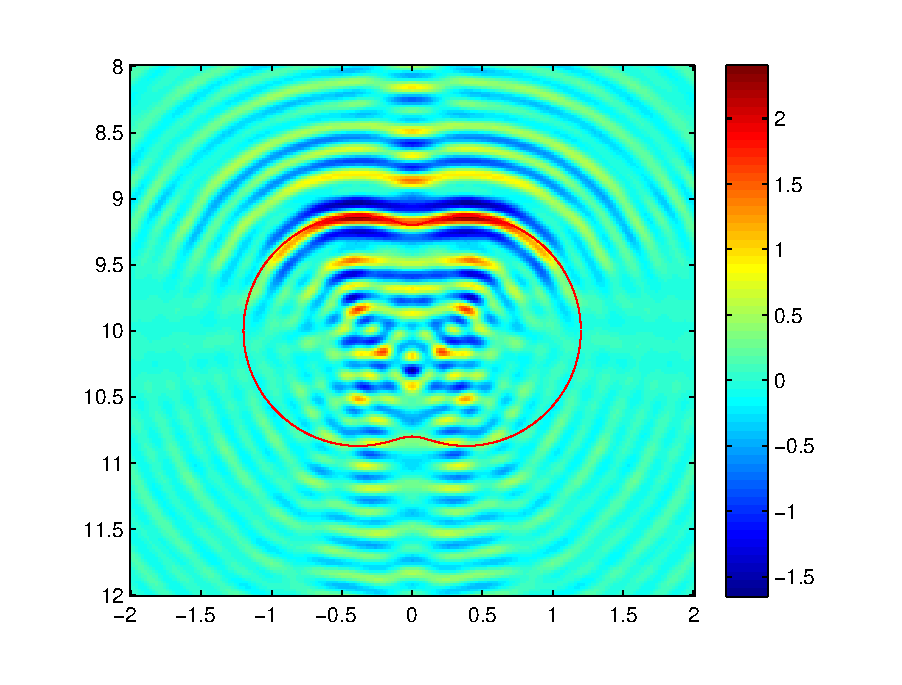
\includegraphics[width=0.24\textwidth]{./graphic/peanut_3pi.eps}
 	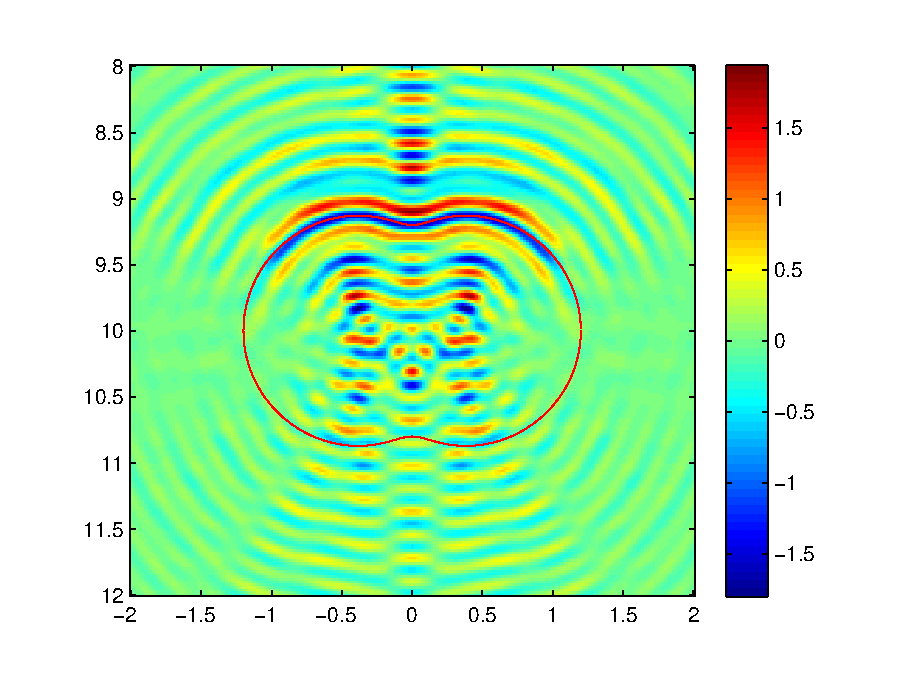
\includegraphics[width=0.24\textwidth]{./graphic/peanut_3pi_neumann.eps}
 	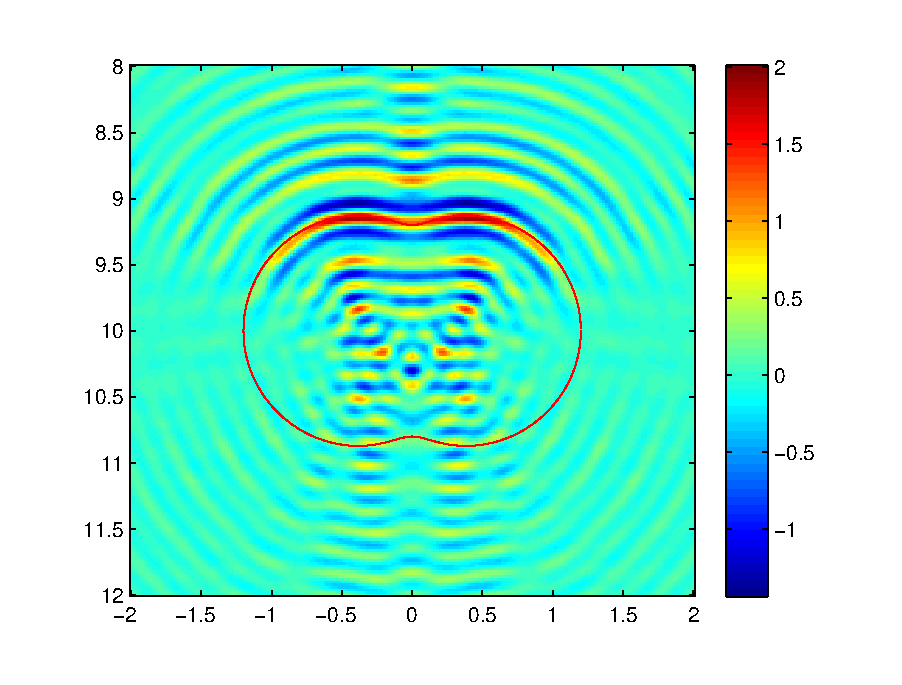
\includegraphics[width=0.24\textwidth]{./graphic/peanut_3pi_impedance_1.eps}
 	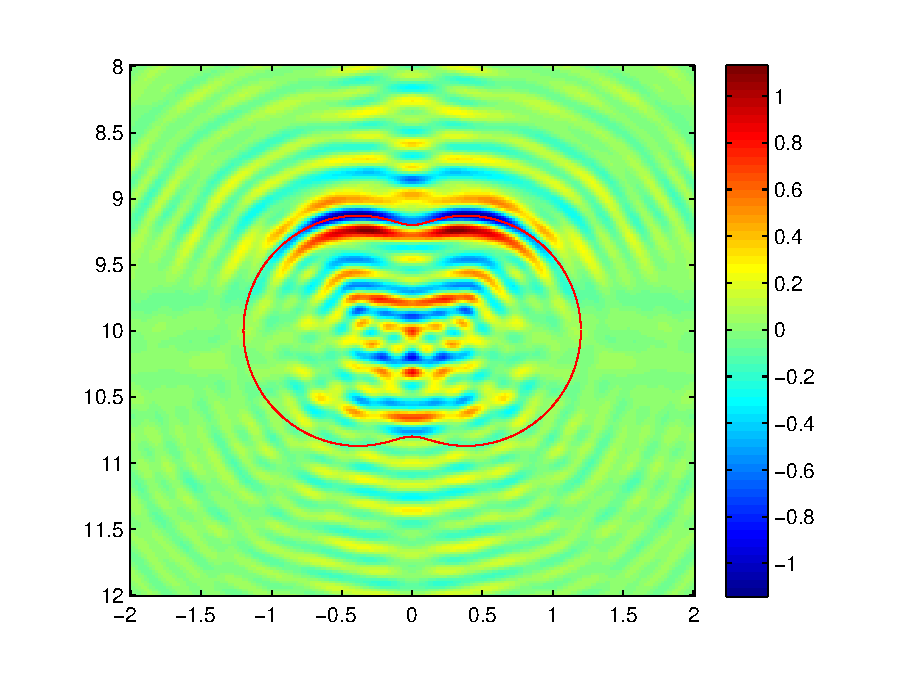
\includegraphics[width=0.24\textwidth]{./graphic/peanut_3pi_transmission.eps}
 	\caption{Example 1: From left to right: imaging results of a Dirichlet, a Neumann, a Robin bounday with impedance $\eta(x)=1$, and a penetrable obstacle with diffractive index $n(x)=0.25$}\label{figure_1}
 \end{figure}
 
 The imaging results are shown in Figure \ref{figure_1}. It demonstrates clearly that our RTM
 algorithm can effectively image the upper boundary illuminated by the sources and
 receivers distributed along the boundary $\Ga_0$ for non-penetrable obstacles. The imaging
 values decrease on the shadow part of the obstacles and at the points away from the
 boundary of the obstacle.

\bigskip
\textbf{Example 2}. We consider the imaging of clamped obstacles with different shapes including circle, peanut, p-leaf and rounded square. The imaging domain is $ = (−2; 2) \times (8; 12)$ with the sampling grid $201 \times 201$ and $N_s = N_r = 401$. The angular frequency is $\om = 3\pi,4\pi$ for the sigle frequency and $\om=\pi\times[2:0.5:8]$ for the test of multiple frequencies.




\begin{figure}
	\centering
	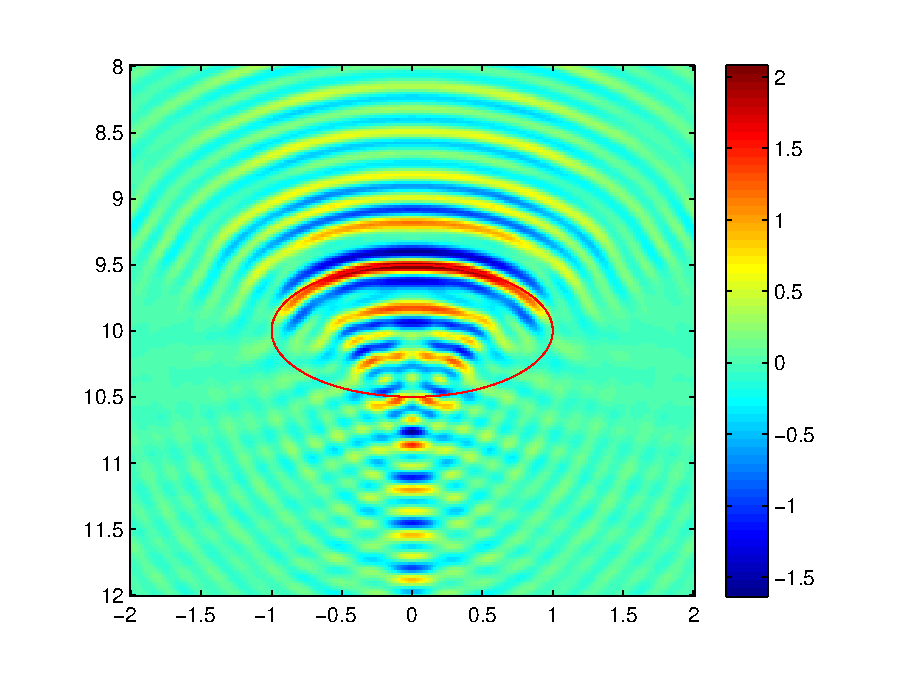
\includegraphics[width=0.32\textwidth]{./graphic/circle_3pi.eps}
	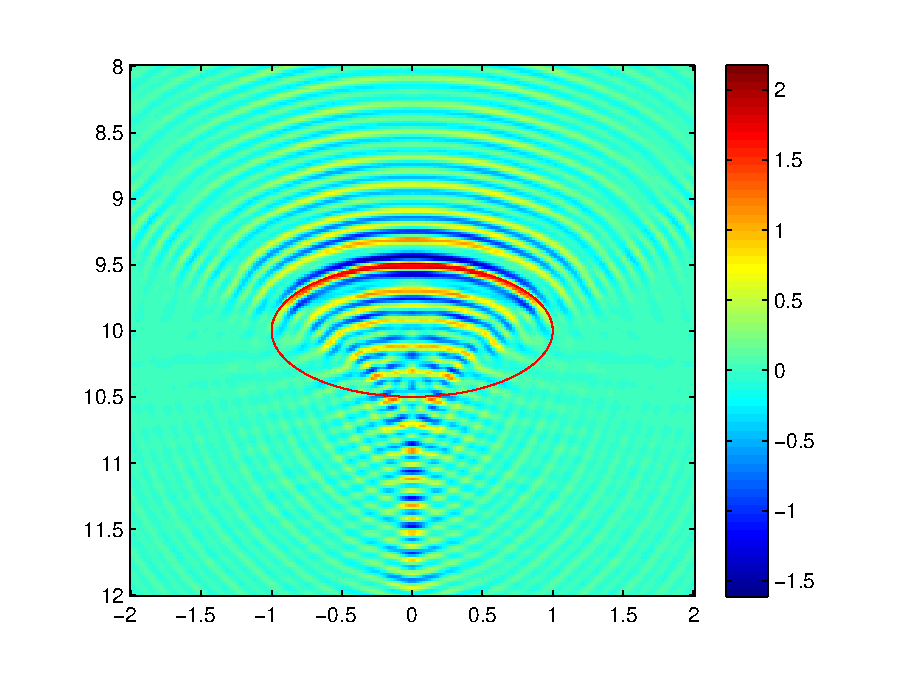
\includegraphics[width=0.32\textwidth]{./graphic/circle_5pi.eps}
	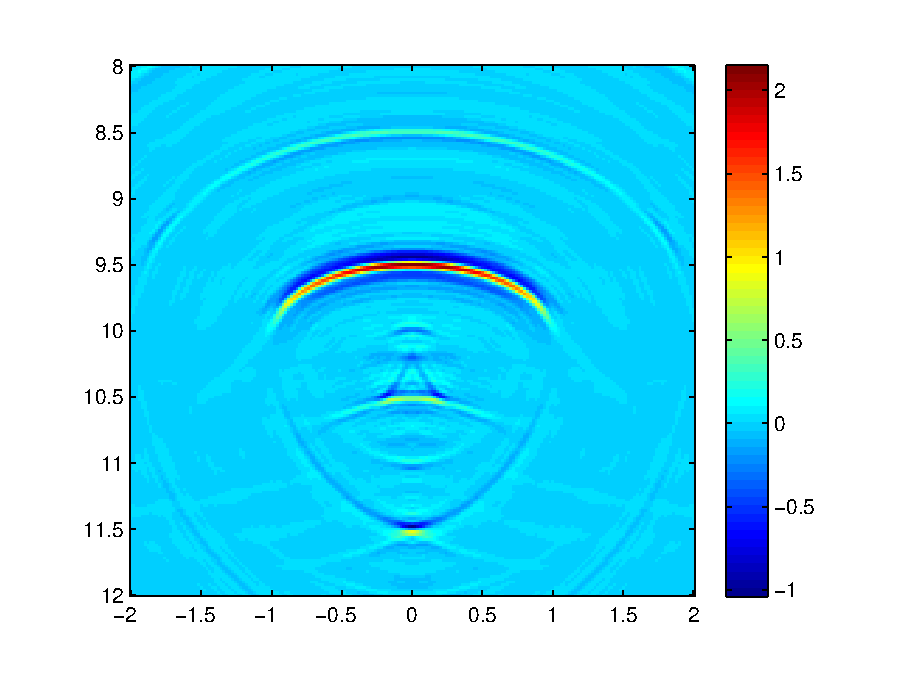
\includegraphics[width=0.32\textwidth]{./graphic/circle.eps}
	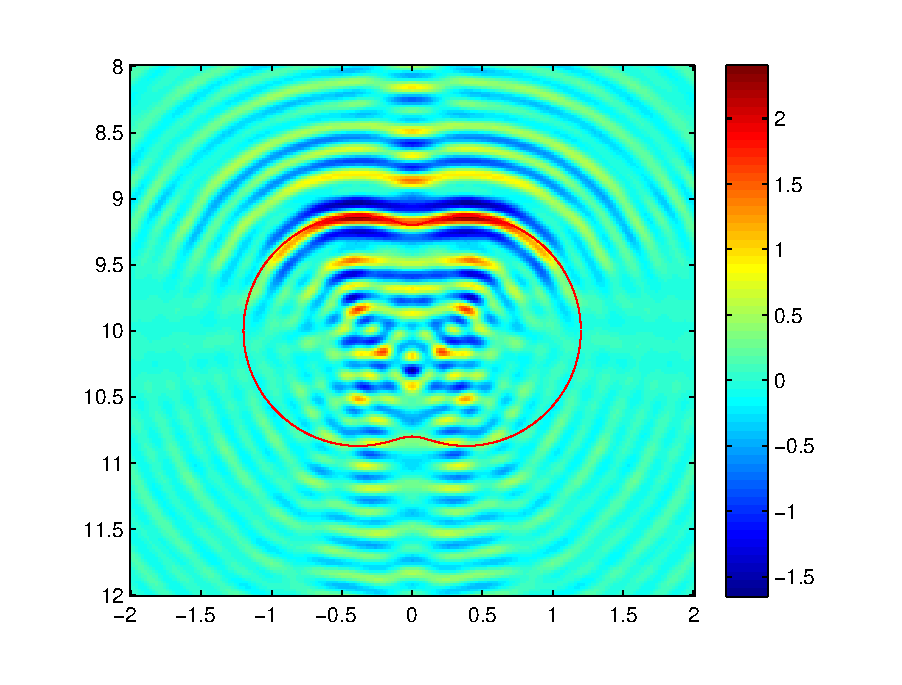
\includegraphics[width=0.32\textwidth]{./graphic/peanut_3pi.eps}
	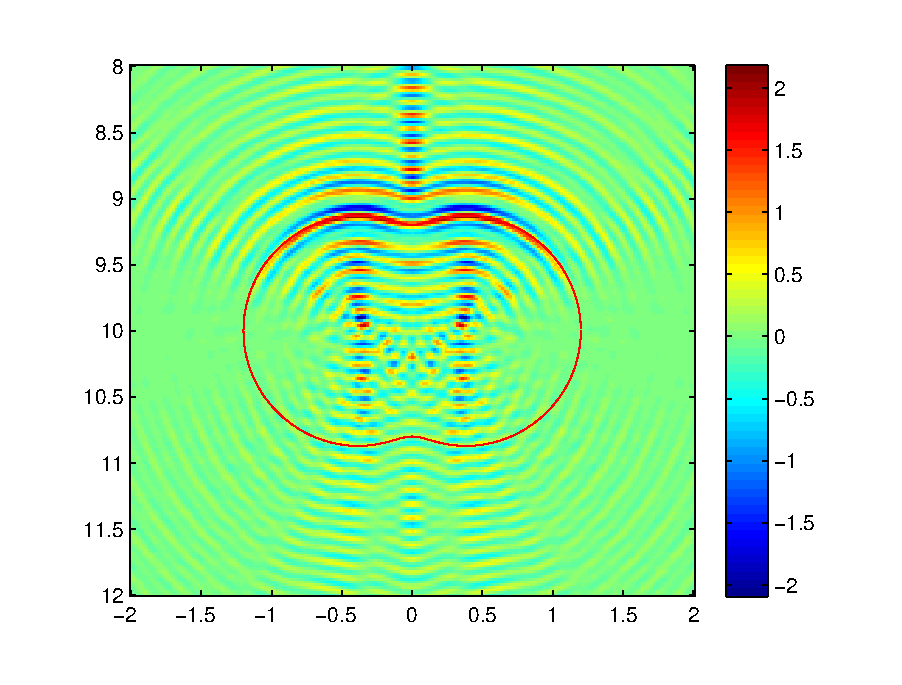
\includegraphics[width=0.32\textwidth]{./graphic/peanut_5pi.eps}
	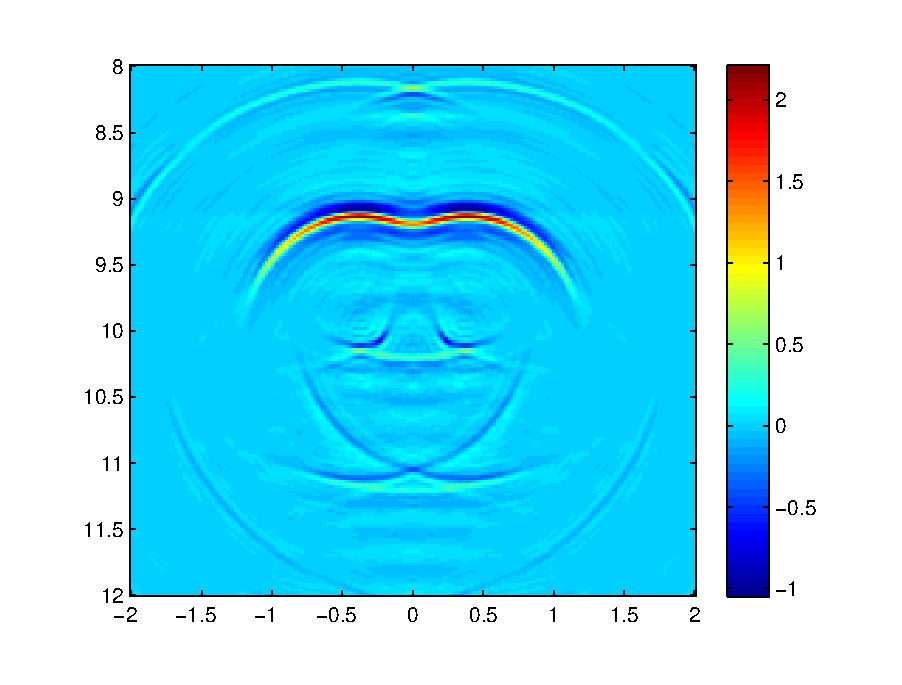
\includegraphics[width=0.32\textwidth]{./graphic/peanut.eps}
	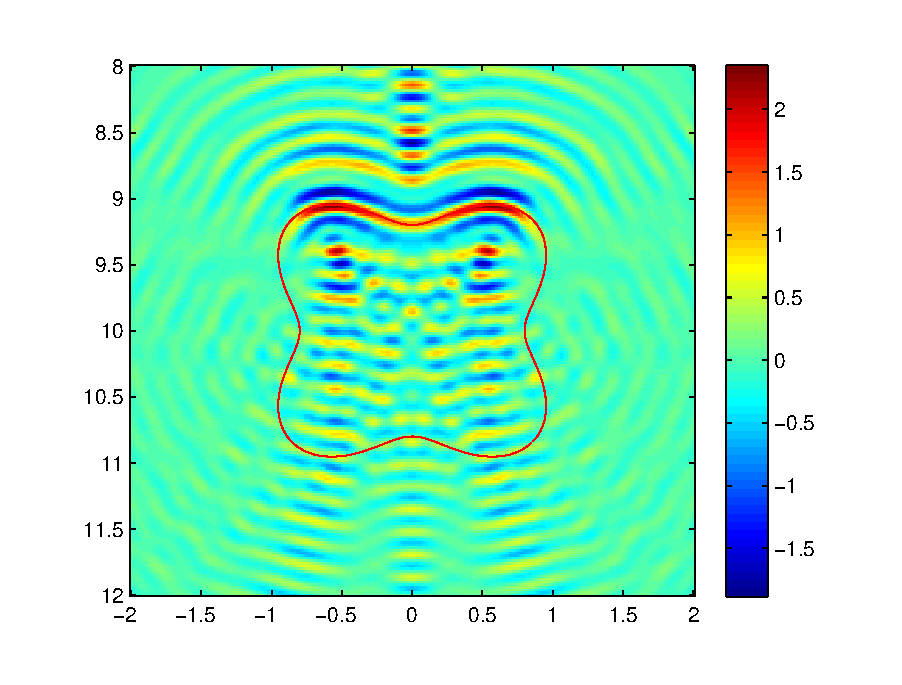
\includegraphics[width=0.32\textwidth]{./graphic/p_leaf_3pi.eps}
	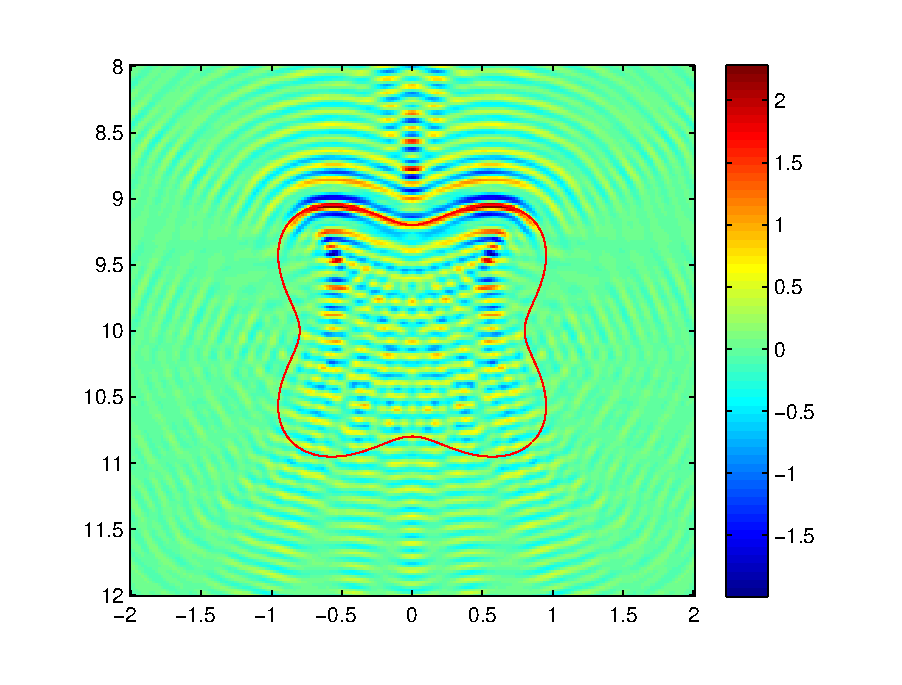
\includegraphics[width=0.32\textwidth]{./graphic/p_leaf_5pi.eps}
	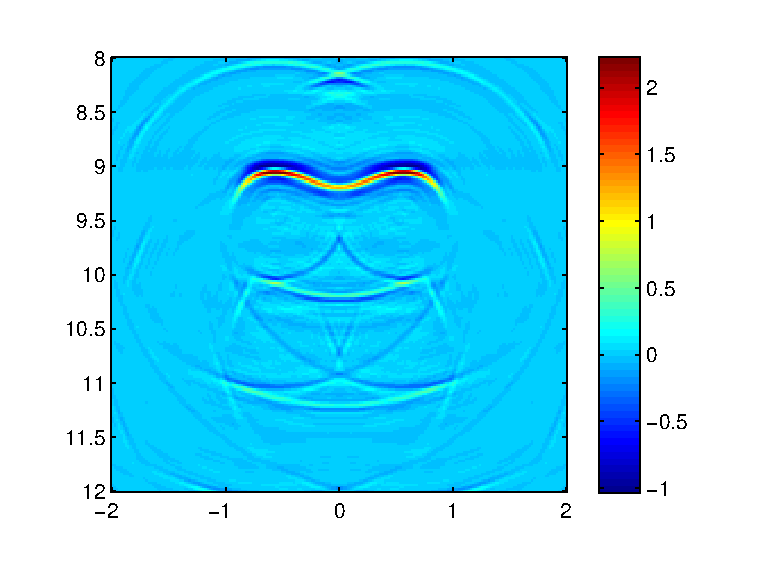
\includegraphics[width=0.32\textwidth]{./graphic/p_leaf.eps}
	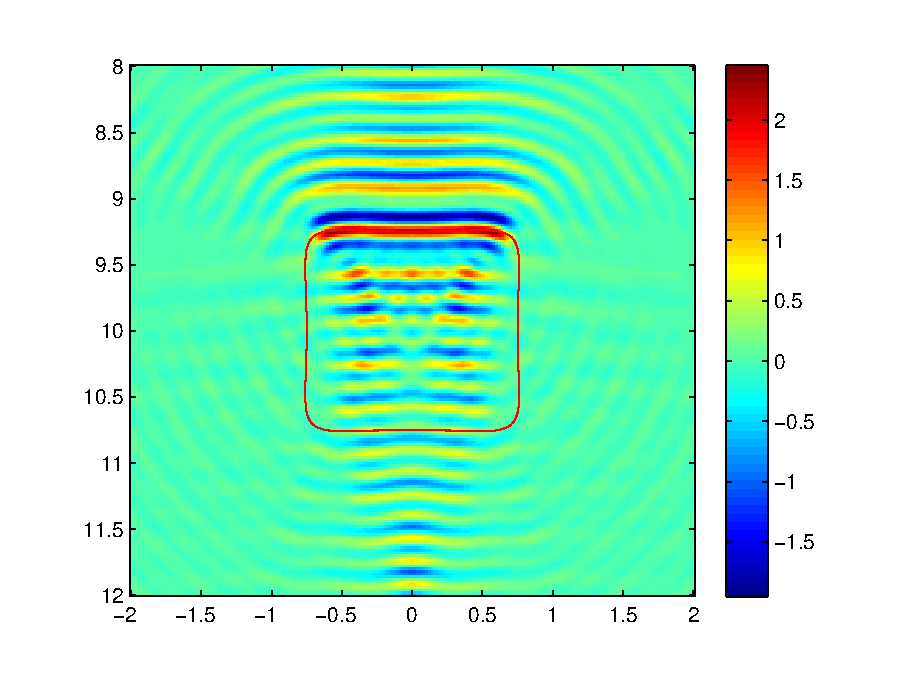
\includegraphics[width=0.32\textwidth]{./graphic/rectangle_3pi.eps}
	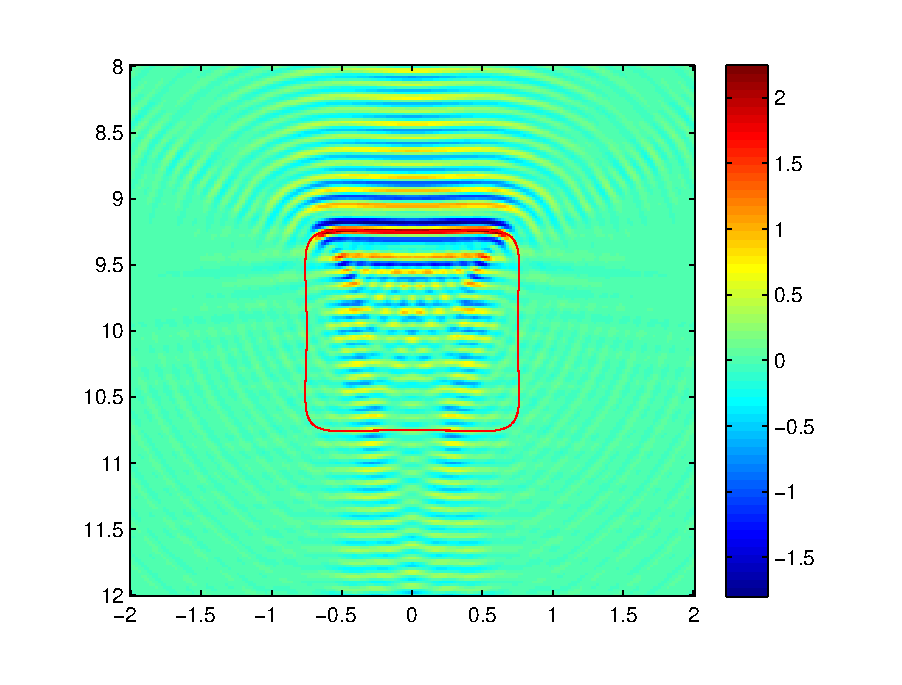
\includegraphics[width=0.32\textwidth]{./graphic/rectangle_5pi.eps}
	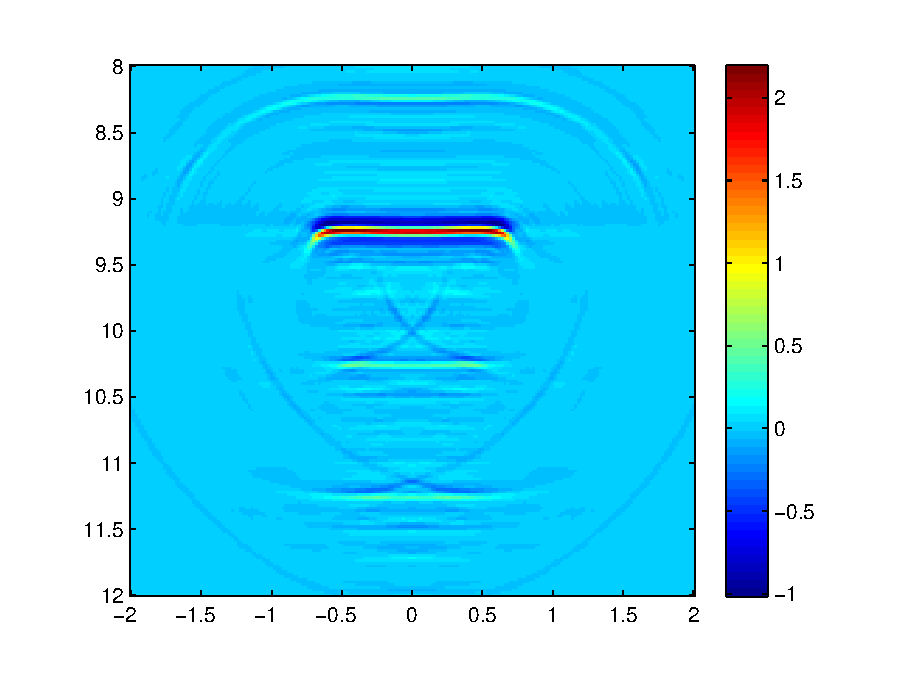
\includegraphics[width=0.32\textwidth]{./graphic/rectangle.eps}
	
	\caption{Example 2: Imaging results of clamped obstacles
		with different shapes from top to below. The left row is imaged with single frequency data where $\om=3\pi$, The middle row is imaged with single frequency data where $\om=5\pi$ and The left row is imaged with multi frequency data}\label{figure_2}
\end{figure}

\bigskip
\textbf{Example 3} We consider the imaging of two sound soft obstacles. The first model
consists of two circles along horizontal direction and the second one is a circle and a
peanut along the vertical direction. The angular frequency is $\om=3\pi$ for the test of the single frequency and $\om=\pi\times[2:0.5:8]$ for the test of multiple frequencies. Figure \ref{figure_31} shows the imaging result of the first model. The
imaging domain is $[−4, 4] \times [8,12]$ with mesh size $401 \times 201$ and $N_s = N_r = 301$. Figure \ref{figure_32}
 shows the imaging result of the second model. The
 imaging domain is $[−4, 4] \times [8,12]$ with mesh size $401 \times 401$ and $N_s = N_r = 301$. The multi-frequency RTM imaging results in Figure \ref{figure_31} and Figure \ref{figure_32} are obtained by adding the inmaging results from different frequencies. We observe from these two figures that imaging results can be greatly improved by stacking the multiple single frequency imaging results. 
\begin{figure}
	\centering
	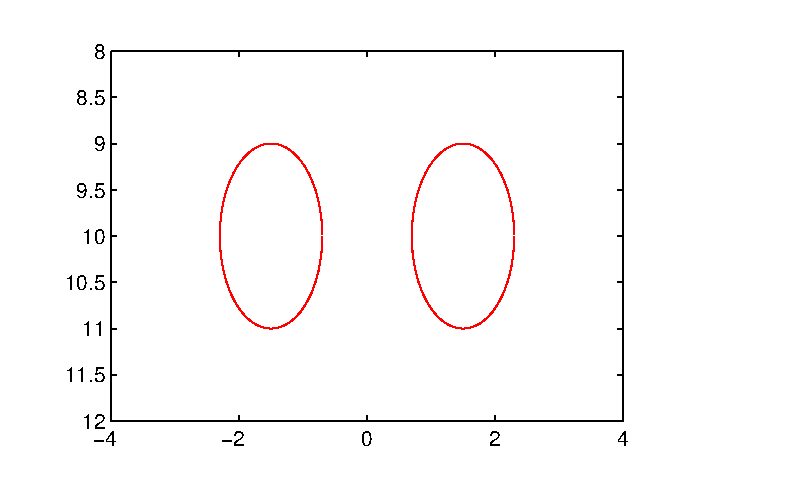
\includegraphics[width=0.32\textwidth,height=0.16\textheight]{./graphic/bi_circle_profile.eps}
	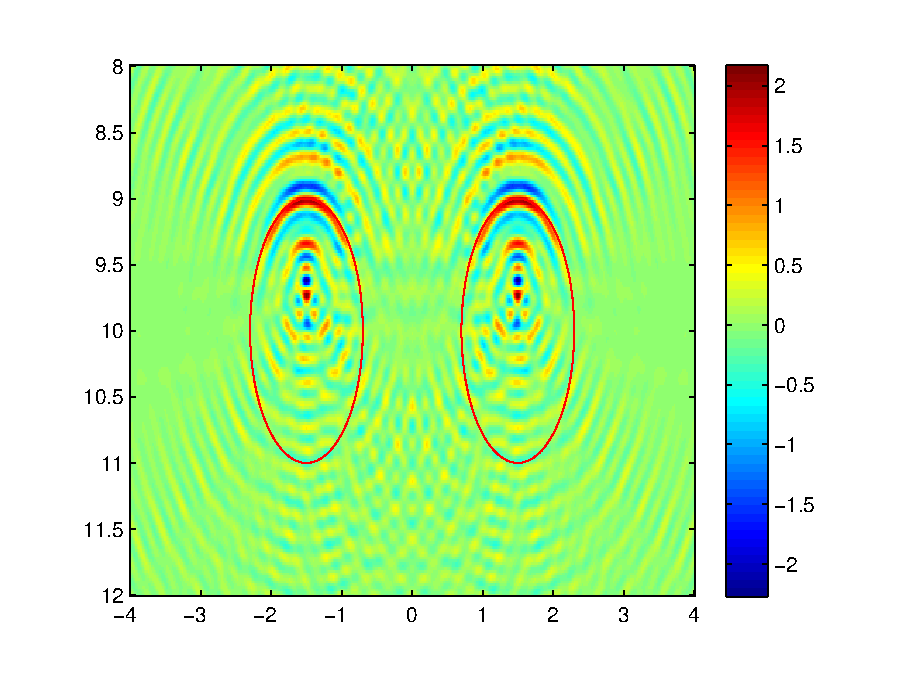
\includegraphics[width=0.32\textwidth]{./graphic/bi_circle_3pi.eps}
	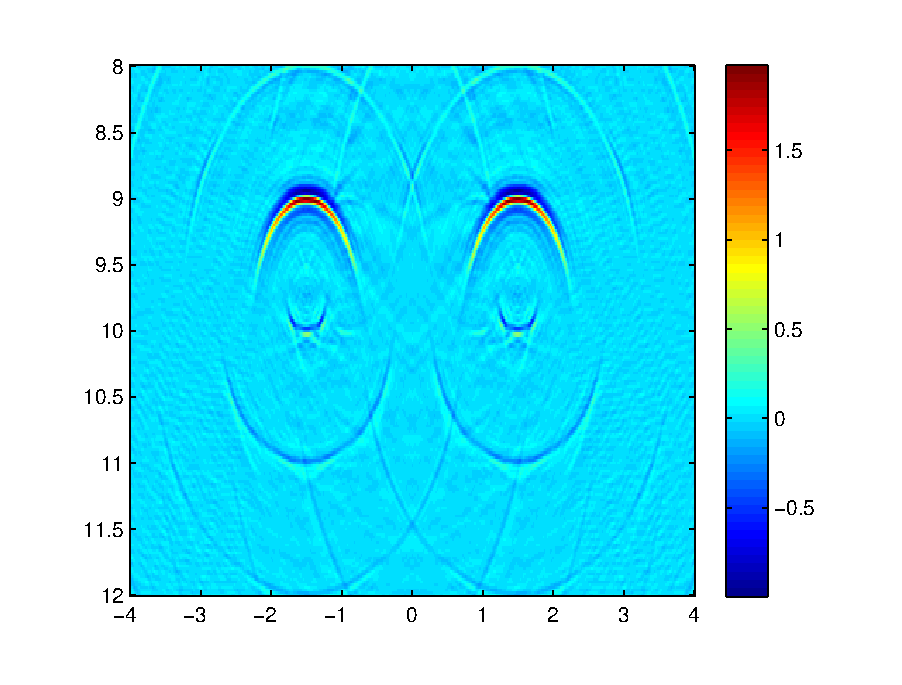
\includegraphics[width=0.32\textwidth]{./graphic/bi_circle.eps}
	
	\caption{Example 3:From left to right,  true obstacle model with two circles. the imaging result
		with single frequency data where $\om=3\pi$, the imaging result with multiple frequency data.}\label{figure_31}
\end{figure}

\begin{figure}
	\centering
	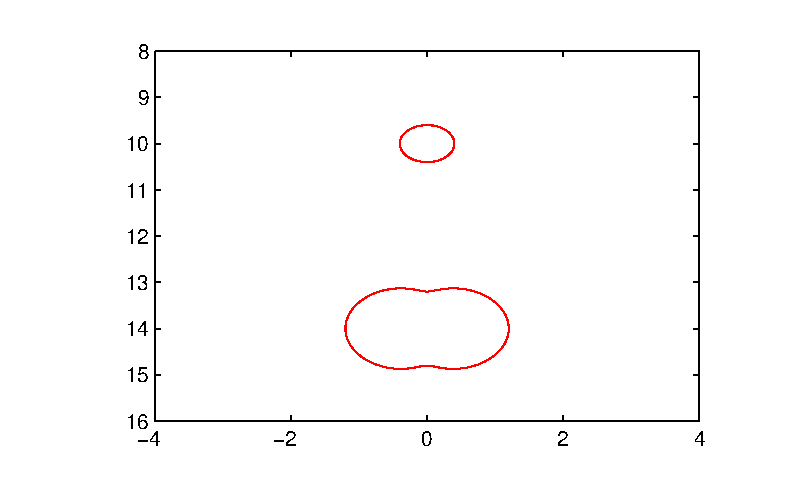
\includegraphics[width=0.32\textwidth,height=0.16\textheight]{./graphic/circle_0_4_peanut_1_profile.eps}
	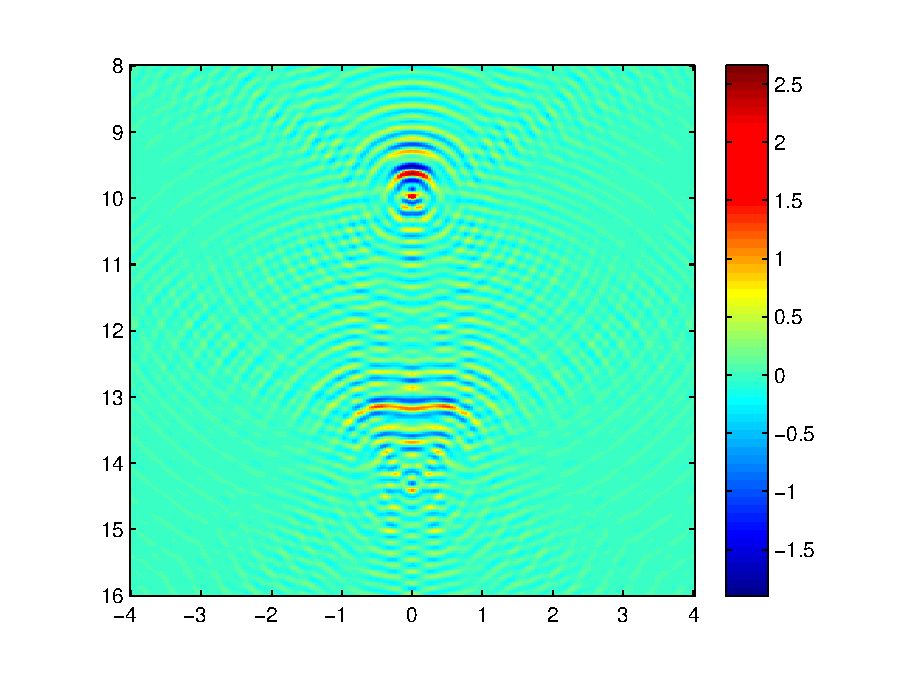
\includegraphics[width=0.32\textwidth]{./graphic/circle_0_4_peanut_1_3pi_1.eps}
	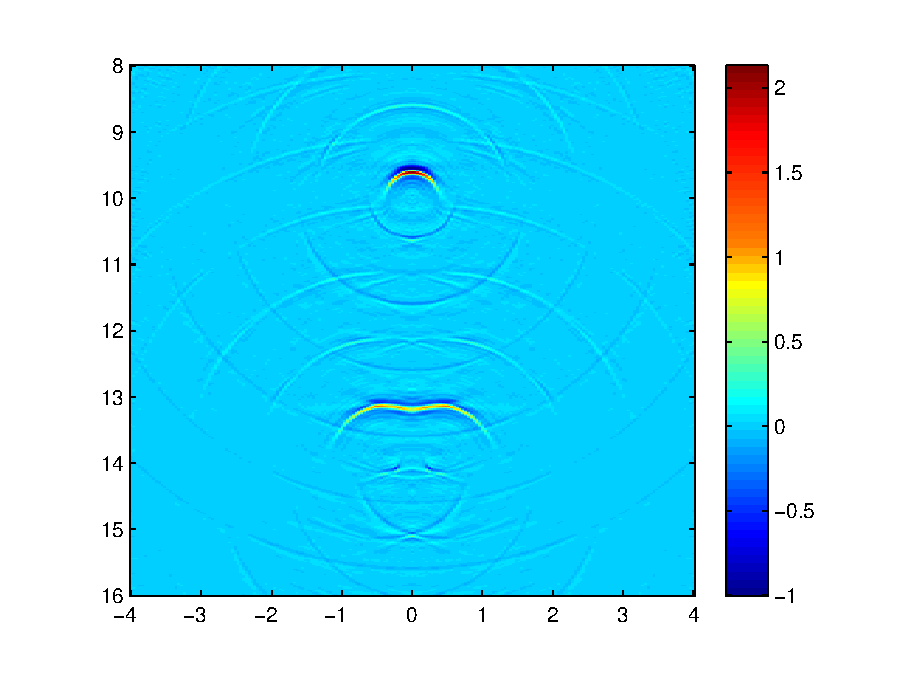
\includegraphics[width=0.32\textwidth]{./graphic/circle_0_4_peanut_1_multi_1.eps}
	
	\caption{Example 3:From left to right,  true obstacle model with one circle and one peanut, the imaging result
		with single frequency data where $\om=3\pi$, the imaging result with multiple frequency data.}\label{figure_32}
\end{figure}

\bigskip
\textbf{Example 4}
In this example we consider the stability of our half space RTM imaging
function with respect to the complex additive Gaussian random noise. We introduce
the additive Gaussian noise as follows
\ben
u_{\rm noise}=u_s+\nu_{\rm noise}
\een
where $u_s$ is the synthesized data and $\nu_{\rm noise}$ is the Gaussian noise with mean zero and standard deviation $\mu$ times the maximum of  the data $|u_s|$, i.e. $\nu_{\rm noise}=\frac{\mu \max |u_s|}{\sqrt{2}}(\ep_1+\i\ep_2)$ and  $\ep_i
\thicksim \mathcal{N}(0,1)$.
\begin{figure}
	\centering
	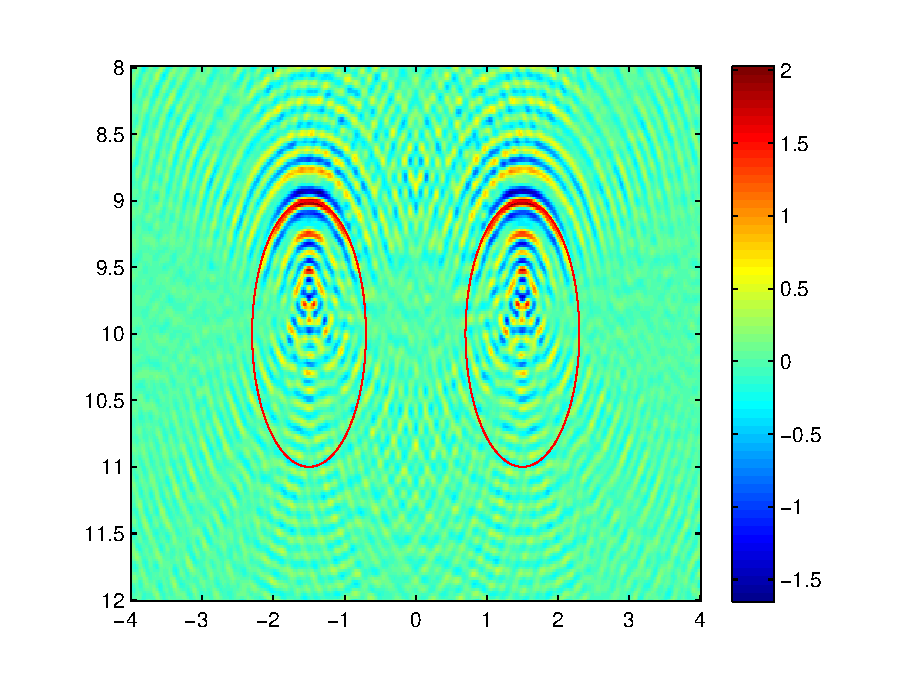
\includegraphics[width=0.32\textwidth]{./graphic/bi_circle_4pi_error2.eps}
	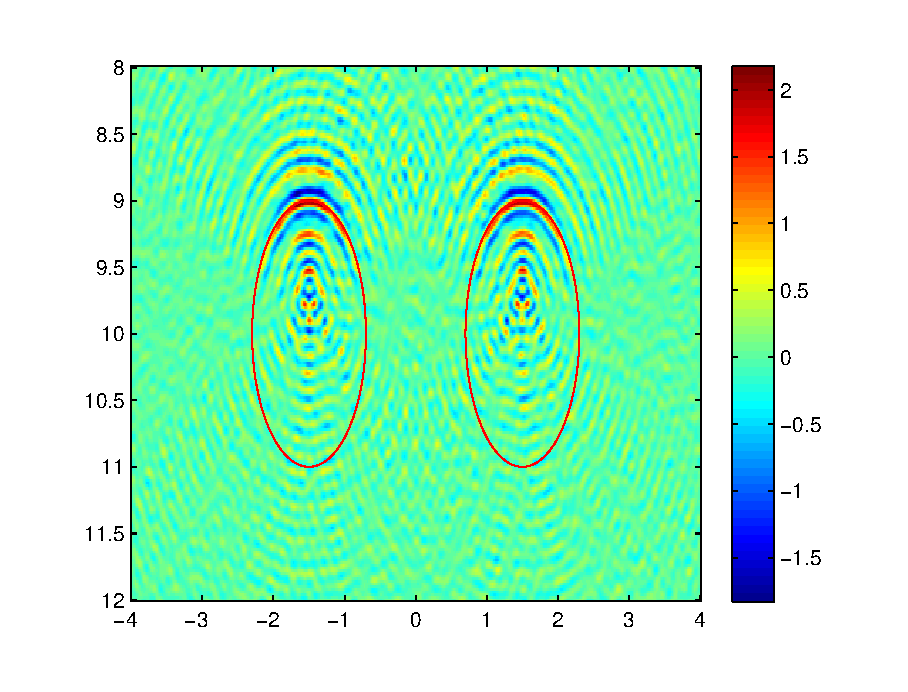
\includegraphics[width=0.32\textwidth]{./graphic/bi_circle_4pi_error4.eps}
	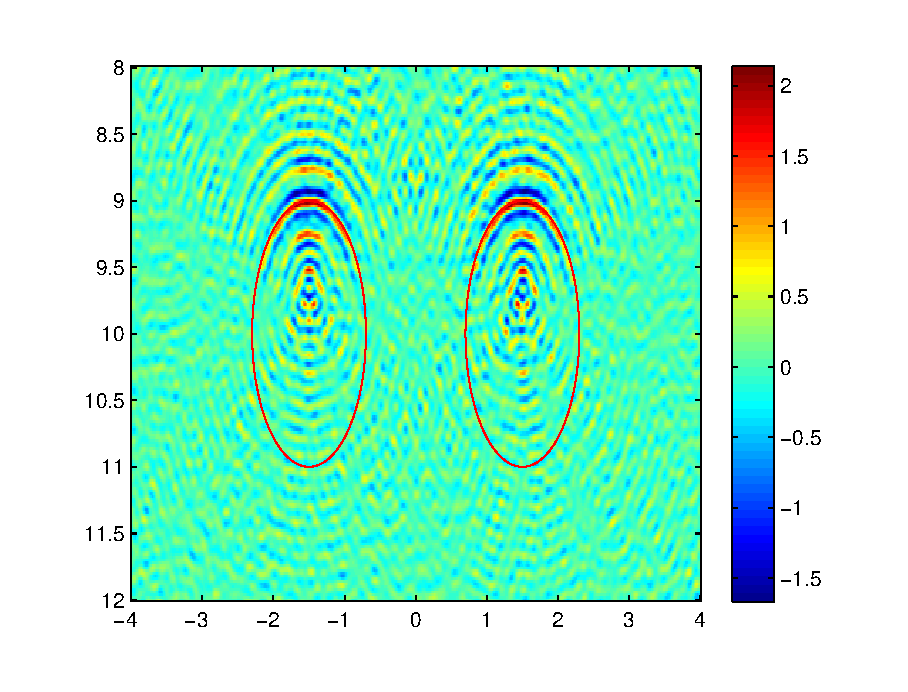
\includegraphics[width=0.32\textwidth]{./graphic/bi_circle_4pi_error6.eps}
	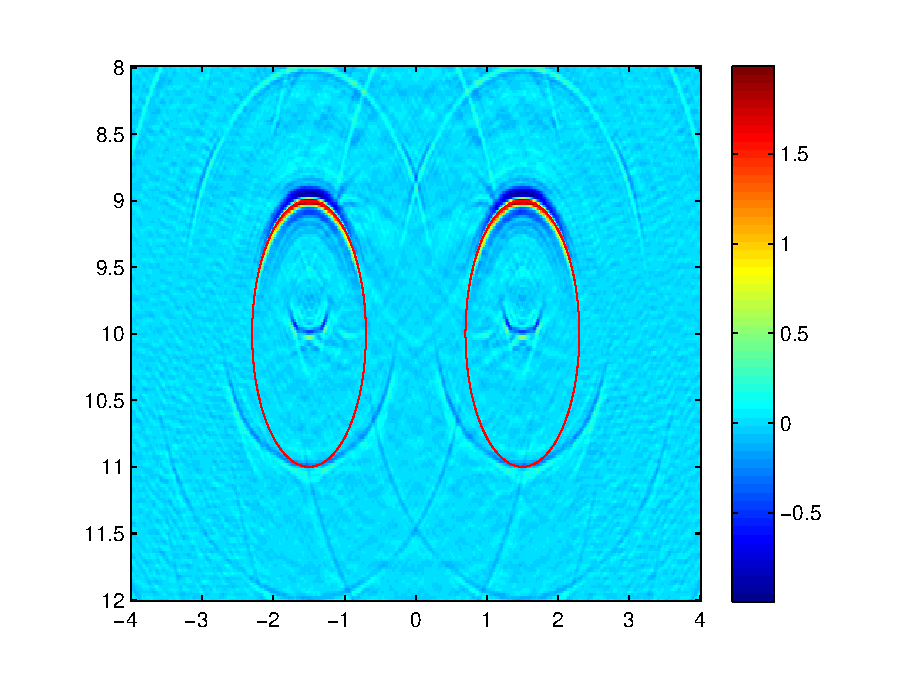
\includegraphics[width=0.32\textwidth]{./graphic/bi_circle_multi_2_8_error2.eps}
	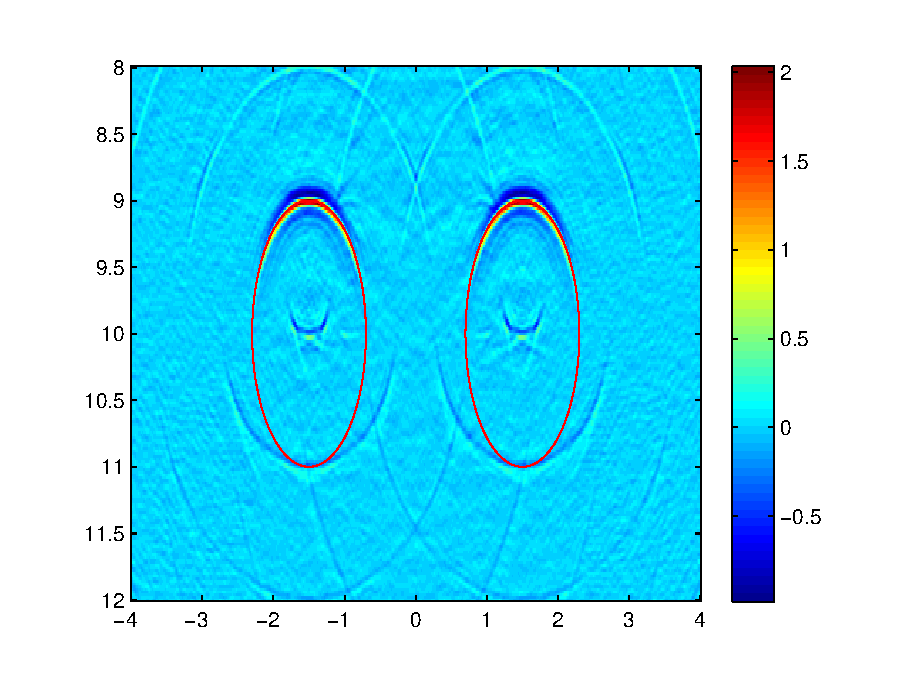
\includegraphics[width=0.32\textwidth]{./graphic/bi_circle_multi_2_8_error4.eps}
	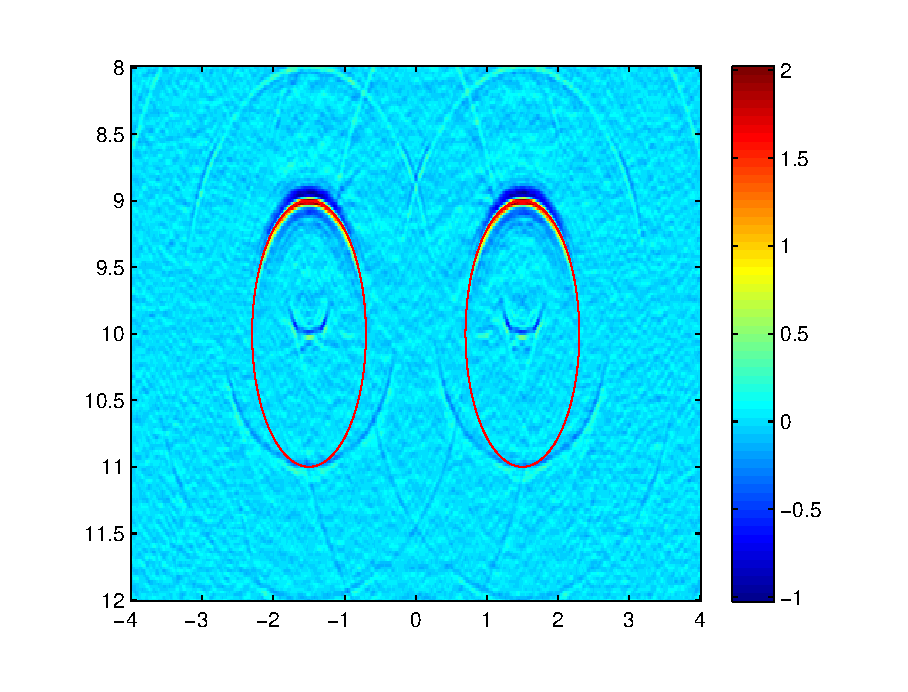
\includegraphics[width=0.32\textwidth]{./graphic/bi_circle_multi_2_8_error6.eps}
	
	\caption{Example 4: Imaging results of a clamped obstacle with noise levels $\mu =  0.2; 0.3; 0.4$ (from left to
		right). The top row is imaged with single frequency data where $\om=4\pi$, and the
		bottom row is imaged with multi-frequency data.}\label{figure_4}
\end{figure}

Figure \ref{figure_4} shows the imaging results using single frequency data added with additive
Gaussian noise. The imaging quality can be improved by using multi-frequency data.
as illustrated 

\section*{References}
\bibliography{eee}
\end{document}
